\chapter{スタートプロジェクトの作成}
\label{chap:02-create-react-app}
\begin{starterabstract}
Reactアプリケーションを作成するための最初のステップとして、トップページのみを持つスタートアッププロジェクトを作成します。
 \\[0pt]

スタートアッププロジェクトを作成する方法として、\\[0pt]
 \\[0pt]
  1. create{-}react{-}app\\[0pt]
  2. ゼロから構築\\[0pt]
 \\[0pt]
の2つの方法を解説します。

 \\[0pt]
「create{-}react{-}app」は、コマンド一発でReactアプリケーション開発が数分で始められます。

 \\[0pt]
ただし、Facebook(Meta社)を中心に開発されている便利なものなのですが、メンドウな設定などが隠されているため
バージョンの合わないライブラリを導入すると整合性が崩れ手に負えなくなることもあります。

 \\[0pt]
2021年12月14日にリリースされた「create{-}react{-}app V5.0.0」では、webpack、eslintなどは最新のものが使われています。

 \\[0pt]
「ゼロから構築」を選択すると、最新のライブラリが使用できますが、webpack、ESLintなどの設定ファイルは自分で書かなくてはなりません。
使用するライブラリの設定自体は難しくないので、ここで勉強しておけば必ず役に立つはずです。

 \\[0pt]
 どちらの方法もGitHubにテンプレートとしてアップロードしてありますので、ご自由にお使いください。

\end{starterabstract}

\section{create{-}react{-}appコマンド}
\keeplastskip{
  \label{sec:2-1}
  \label{sec-01command}
  \par\nobreak
}

Reactアプリケーションをゼロから作成するためには、

\begin{starteritemize}
\item 「nodeプロジェクト」に必要なpackage.jsonを作成
\item reactなど必要なライブラリのインストール
\item 作成したアプリケーションが、古いブラウザでも実行できるようにコードを変換(Babel使用)
\item 出力するファイルをまとめる(バンドルする {-} webpack使用)
\end{starteritemize}

など、reactライブラリのインストール以外にも、Babelやwebpackをインストールして設定ファイルを作成しなくてはなりません。

\vspace*{\baselineskip}

また、使用するライブラリによっては、プラグインのインストールや設定など、アプリケーションのコードを書き始める前の作業がたいへんです。

\vspace*{\baselineskip}

しかし、「そんなメンドウなことは、やってられない。」と誰しもが思ったか、
すぐにでもコードを書き始めることのできるスタート用アプリケーションが、react開発元のFacebook(Meta)から提供されています。

\vspace*{\baselineskip}

さらに、そのスタート用アプリケーションは、コマンド一発でインストールできます。

\vspace*{\baselineskip}

では、実際に手を動かしましょう。
ターミナルを起動し、プロジェクトを作成するフォルダへ移動します。

\def\startercodeblockfontsize{}
\begin{starterterminal}[]{create{-}react{-}appでスタート用アプリケーション作成}\seqsplit{\textgreater{} npx create react{-}app プロジェクト名 {-}{-}template typescript}\end{starterterminal}

エンターキーを押すと、作業が始まり「プロジェクト名」のフォルダが作成され、
以下のように表示されればスグにでも開発に取りかかれます。

\def\startercodeblockfontsize{}
\begin{starterterminal}[]{create{-}react{-}app完了時}\seqsplit{  Success! Created yaruo{-}cra{-}template at /Users/yaruo/yaruo{-}cra{-}template
  Inside that directory, you can run several commands:

    npm start
      Starts the development server.

    npm run build
      Bundles the app into static files for production.

    npm test
      Starts the test runner.

    npm run eject
      Removes this tool and copies build dependencies, configuration files
      and scripts into the app directory. If you do this, you can’t go back!

  We suggest that you begin by typing:

    cd yaruo{-}cra{-}template
    npm start

  Happy hacking!}\end{starterterminal}
\begin{starterquote}

「create{-}react{-}app」は、2021年12月14日にV5.0.0がリリースされました。
このリリースでは、メジャーバージョンアップされていた「webpack5」、「eslint8」が採用されています。

\end{starterquote}
\begin{starternote}[]{github}

ここまでの作業は、GitHubにあります。

\def\startercodeblockfontsize{}
\begin{starterterminal}[]{GitHubから}\seqsplit{\textgreater{} git clone {-}b 01\textunderscore{}create{-}react{-}app{-}executed https://github.com/yaruo{-}react{-}redux/yaruo{-}cra{-}template.git}\end{starterterminal}
\end{starternote}

\subsection{アプリケーションを実行}
\keeplastskip{
  \label{sec:2-1-1}
  \label{sec-02yarnstart}
  \par\nobreak
}

アプリケーションが作成できましたので、実行してみます。

ターミナルの表示に従い、プロジェクトフォルダへ移動し、スタート用のコマンドを入力します。

\def\startercodeblockfontsize{}
\begin{starterterminal}[]{プロジェクトの実行}\seqsplit{ \textgreater{} cd プロジェクト名
 \textgreater{} npm run start {\reviewballoon{もしくは、yarn start}}}\end{starterterminal}

すると、webpackに同梱されている開発用のweb serverが起動し、デフォルトでは、port:3000でアプリケーションへアクセスできます。

\def\startercodeblockfontsize{}
\begin{starterterminal}[]{npm run start時}\seqsplit{Compiled successfully!

You can now view yourproject in the browser.

  Local:            http://localhost:3000
  On Your Network:  http://pcのローカルIPアドレス:3000

Note that the development build is not optimized.
To create a production build, use yarn build.}\end{starterterminal}

Google Chromeが起動し、http://localhost:3000へアクセスし以下のページが表示されます。

\begin{reviewimage}[H]%%02_cra_start
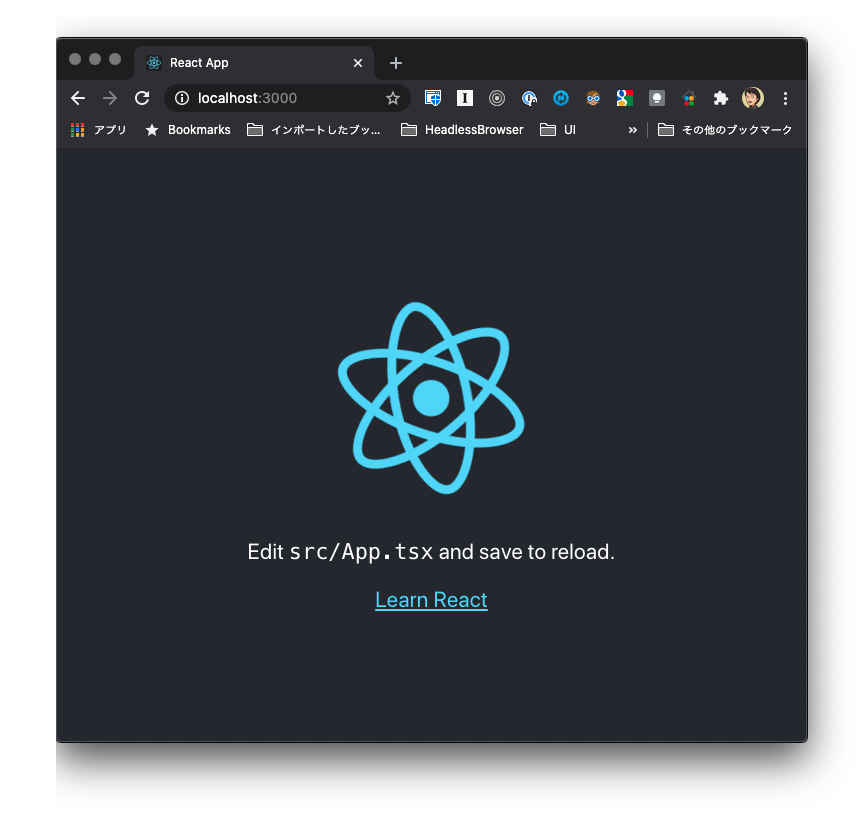
\includegraphics[width=1.0\maxwidth]{./images/02-create-react-app/02_cra_start.png}%
\reviewimagecaption{create{-}react{-}appの画面}
\label{image:02-create-react-app:02_cra_start}
\end{reviewimage}

このページが表示されれば成功です。

\subsection{create{-}react{-}appで作成された中身}
\keeplastskip{
  \label{sec:2-1-2}
  \label{sec-03cra-desc}
  \par\nobreak
}

create{-}react{-}appで作成された中身は、以下となります(使用するテンプレートにより作成されるファイル・フォルダは異なる)。

\def\startercodeblockfontsize{}
\begin{starterterminal}[]{create{-}react{-}appで作成されたファイル・フォルダ}\seqsplit{  .
  ├── node\textunderscore{}modules
  ├── README.md
  ├── package{-}lock.json
  ├── package.json
  ├── public
  │   ├── favicon.ico
  │   ├── index.html
  │   ├── logo192.png
  │   ├── logo512.png
  │   ├── manifest.json
  │   └── robots.txt
  ├── src
  │   ├── App.css
  │   ├── App.test.tsx
  │   ├── App.tsx
  │   ├── index.css
  │   ├── index.tsx
  │   ├── logo.svg
  │   ├── react{-}app{-}env.d.ts
  │   ├── reportWebVitals.ts
  │   └── setupTests.ts
  └── tsconfig.json}\end{starterterminal}

package.jsonファイルは、Node.jsを使用するプロジェクトの設計図にあたるものです。

\vspace*{\baselineskip}

Node.jsを使うプロジェクトを開始する場合には、プロジェクトフォルダで「npm init」を行うと対話形式で「package.json」を作成しますが、
create{-}react{-}appコマンドを使用すると、package.jsonも以下のように作成されます。

\def\startercodeblockfontsize{}
\begin{starterprogram}[]{package.json}\seqsplit{  \{
    "name": "作成時に入力したプロジェクト名",
    "version": "0.1.0",
    "private": true,
    "dependencies": \{
      "@testing{-}library/jest{-}dom": "\textasciicircum{}5.16.1",
      "@testing{-}library/react": "\textasciicircum{}12.1.2",
      "@testing{-}library/user{-}event": "\textasciicircum{}13.5.0",
      "@types/jest": "\textasciicircum{}27.0.3",
      "@types/node": "\textasciicircum{}16.11.14",
      "@types/react": "\textasciicircum{}17.0.37",
      "@types/react{-}dom": "\textasciicircum{}17.0.11",
      "react": "\textasciicircum{}17.0.2",
      "react{-}dom": "\textasciicircum{}17.0.2",
      "react{-}scripts": "5.0.0",
      "typescript": "\textasciicircum{}4.5.4",
      "web{-}vitals": "\textasciicircum{}2.1.2"
    \},
    "scripts": \{
      "start": "react{-}scripts start",
      "build": "react{-}scripts build",
      "test": "react{-}scripts test",
      "eject": "react{-}scripts eject"
    \},
    "eslintConfig": \{
      "extends": [
        "react{-}app",
        "react{-}app/jest"
      ]
    \},
    "browserslist": \{
      "production": [
        "\textgreater{}0.2\%",
        "not dead",
        "not op\textunderscore{}mini all"
      ],
      "development": [
        "last 1 chrome version",
        "last 1 firefox version",
        "last 1 safari version"
      ]
    \}
  \}}\end{starterprogram}

package.json内にある「scripts」にあるものがコマンドになります。react{-}scriptsは、npmスクリプトを連続、
または、並列に実行してくれるものです。

\vspace*{\baselineskip}

package.jsonの「dependencies」には、実行に必要でインストール済みのnpmパッケージが記載されています。
必要なnpmパッケージをインストールすると、ここに自動的に追記されます。

\vspace*{\baselineskip}

また、開発時のみ必要なパッケージ(buildしたときには組み込まれない)は、「devDependencies」に追加されます。

\section{ ゼロから構築してみる}
\keeplastskip{
  \label{sec:2-2}
  \label{sec-04-start}
  \par\nobreak
}

本章では、最新のライブラリを使用してゼロからReact/TypeScriptの環境を構築します。

ステップ毎にGitHub上でブランチを作成してありますので、どこからでも始めていただけます。

\subsection{ステップ1 Node.jsプロジェクト作成}
\keeplastskip{
  \label{sec:2-2-1}
  \label{sec-04-node_init}
  \par\nobreak
}

新しくプロジェクト用のフォルダを作成し移動します。

コンソールで「npm init {-}y」コマンドを実行します。オプションの「{-}y」なしで実行すると、対話形式で「package.json」を作成できます。

\def\startercodeblockfontsize{}
\begin{starterterminal}[]{nodeプロジェクトの開始}\seqsplit{  ❯ npm init {-}y
  Wrote to /Users/yaruo/Documents/yaruo\textunderscore{}react\textunderscore{}sample/yaruo{-}start{-}template/package.json:

  \{
    "name": "yaruo{-}start{-}template",
    "version": "1.0.0",
    "description": "",
    "main": "index.js",
    "scripts": \{
      "test": "echo \reviewbackslash{}"Error: no test specified\reviewbackslash{}" \&\& exit 1"
    \},
    "repository": \{
      "type": "git",
      "url": "git+https://github.com/yaruo{-}react{-}redux/yaruo{-}start{-}template.git"
    \},
    "keywords": [],
    "author": "",
    "license": "ISC",
    "bugs": \{
      "url": "https://github.com/yaruo{-}react{-}redux/yaruo{-}start{-}template/issues"
    \},
    "homepage": "https://github.com/yaruo{-}react{-}redux/yaruo{-}start{-}template\#readme"
  \}}\end{starterterminal}

作成された「package.json」が表示されます。

\begin{starternote}[]{}

ここまでの内容は、GitHub上で、以下のコマンドでクローンできます。

\def\startercodeblockfontsize{}
\begin{starterterminal}[]{GitHub}\seqsplit{\textgreater{} git clone {-}b 01\textunderscore{}start{-}node{-}project https://github.com/yaruo{-}react{-}redux/yaruo{-}start{-}template.git}\end{starterterminal}
\end{starternote}

\subsection{webpackのインストールと設定}
\keeplastskip{
  \label{sec:2-2-2}
  \label{sec-04-webpack}
  \par\nobreak
}
\begin{reviewimage}%%02_webpack_site
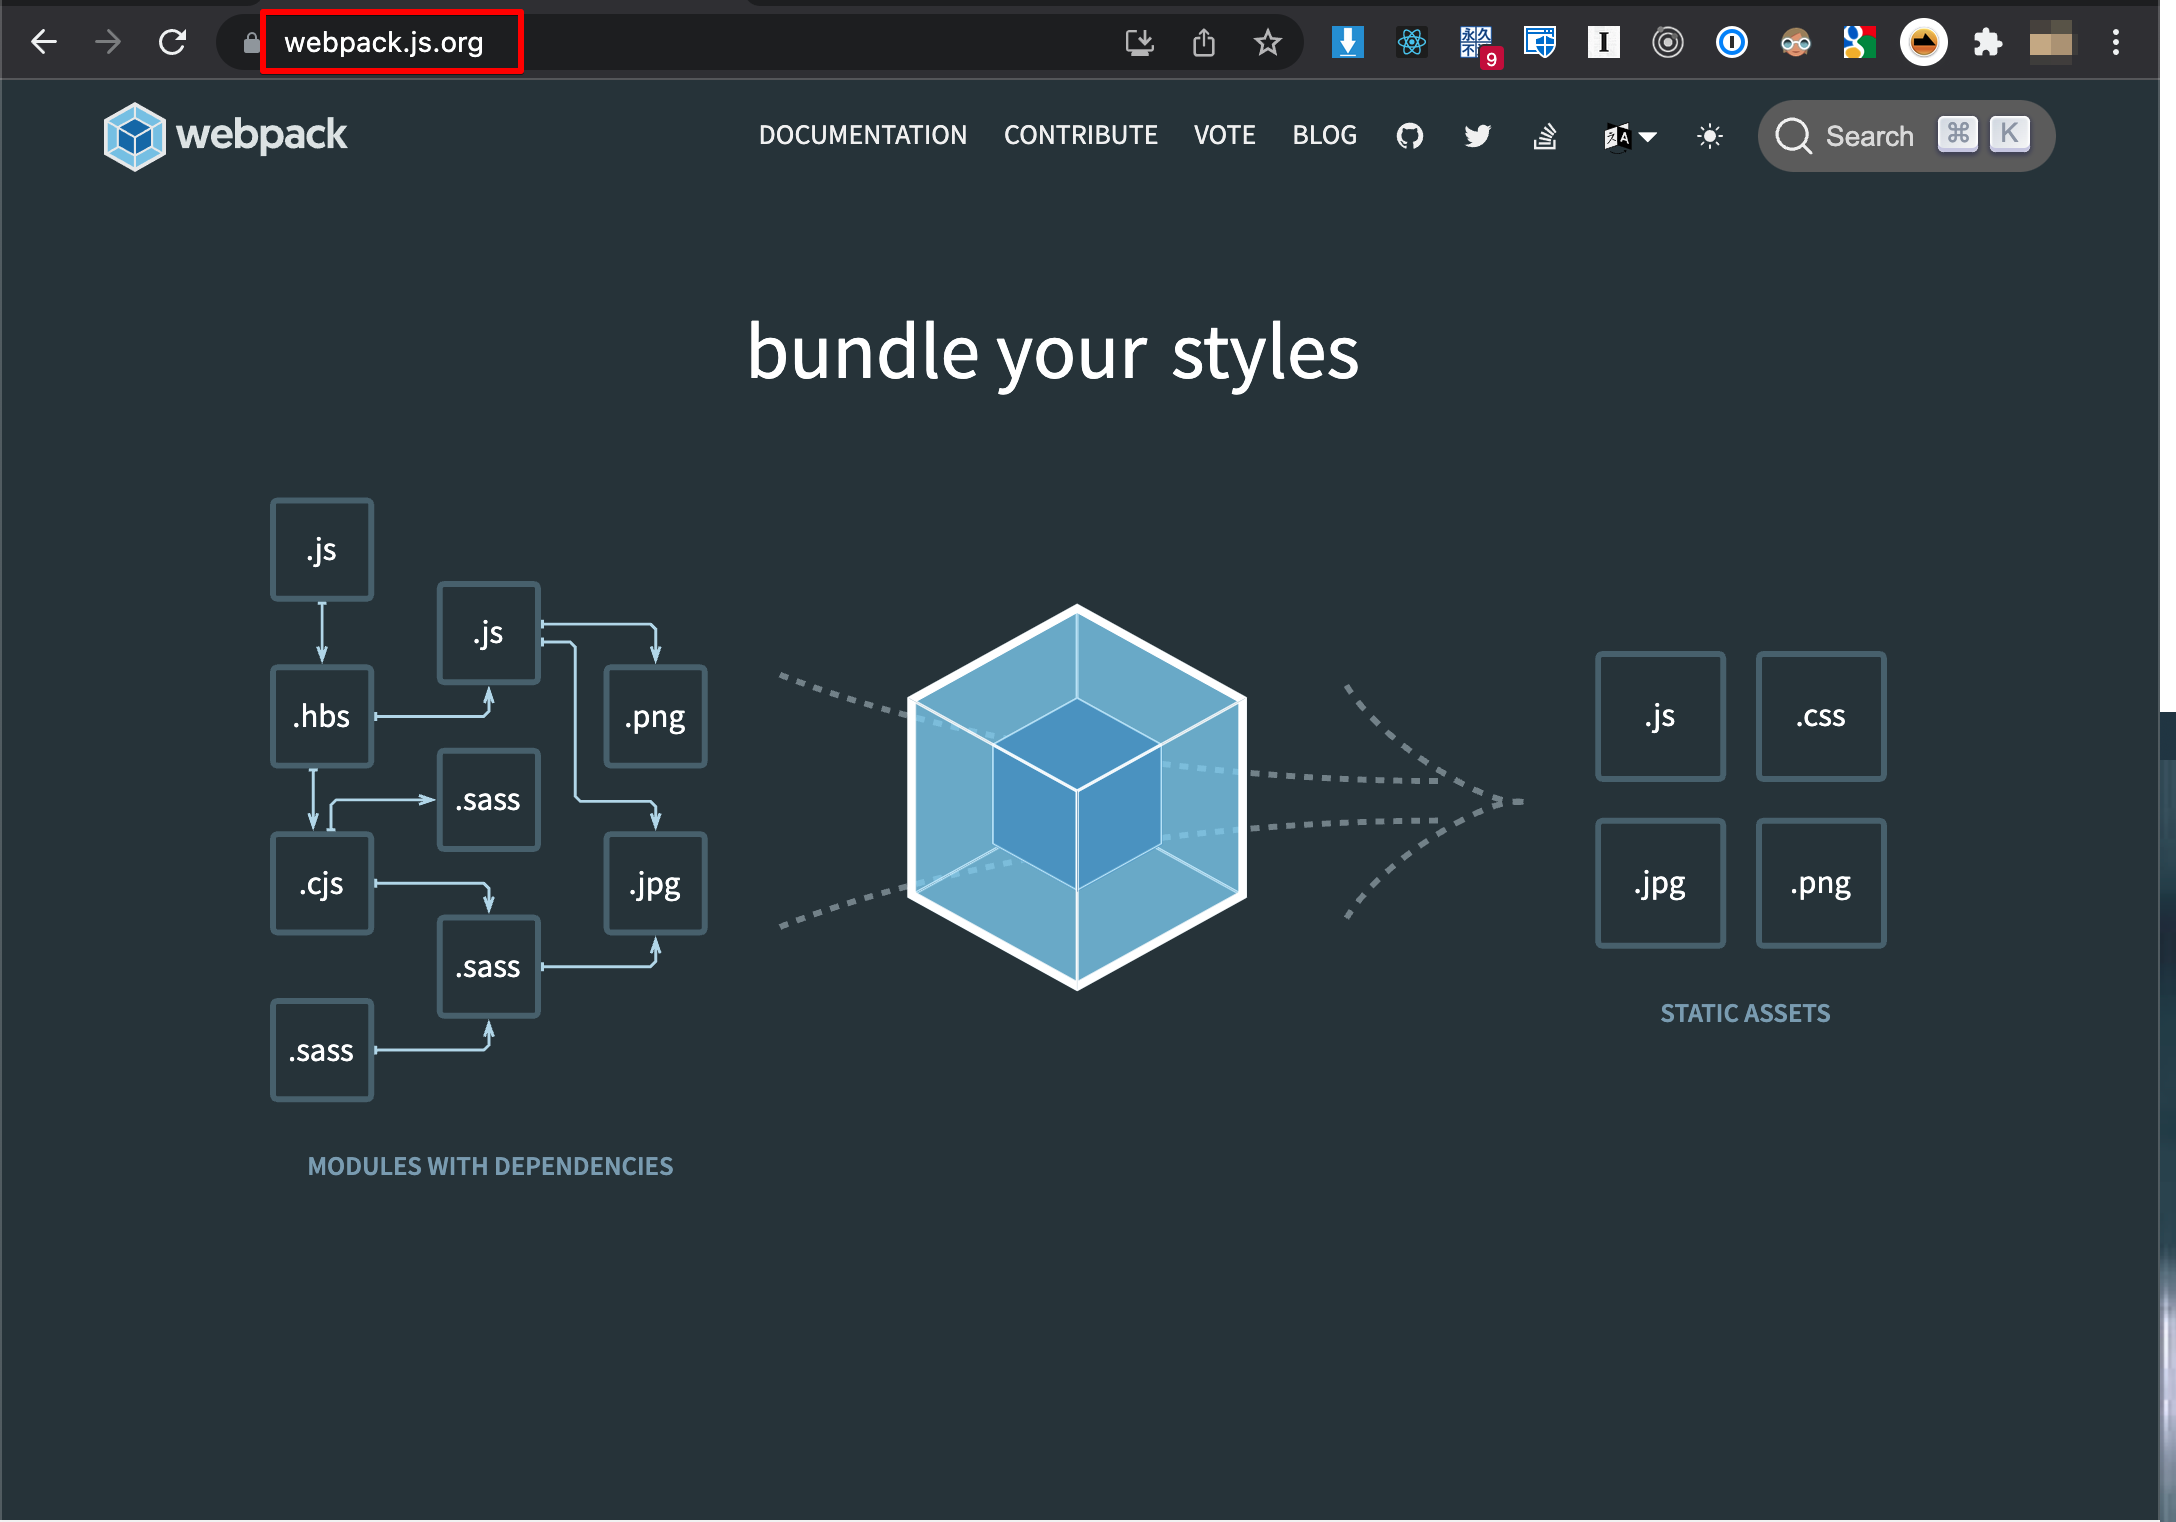
\includegraphics[width=1.0\maxwidth]{./images/02-create-react-app/02_webpack_site.png}%
\reviewimagecaption{desc}
\label{image:02-create-react-app:02_webpack_site}
\end{reviewimage}

webpackとは、(本家\footnote{\url{https://webpack.js.org/}})のトップにある上図が示しているように、

\begin{starteritemize}
\item JavaScriptファイル
\item CSS(SASS,SCSS)ファイル
\item 画像ファイル
\end{starteritemize}

などをすべてJavaScriptファイルとして扱い、インストールしているライブラリファイルなどもすべて含めて
1つのファイルとして出力するバンドラー(まとめる)です。

\vspace*{\baselineskip}

しかし、すべてを1つのファルとするよりも「htmlファイル」、「cssファイル」、画像ファイルを別ファイルとして出力し、
ブラウザがファイルを並列にダウンロードできると効率がよくなり、表示速度も速くなります。
そのため、上図のように、複数ファイルに出力します。

\vspace*{\baselineskip}

それでは、webpackをインストールし、バンドラーの動きを確認しながら設定ファイルを作成していきます。

\vspace*{\baselineskip}

ターミナルに以下のコマンドを入力します。「{-}D(または、{-}{-}save{-}dev)」のオプションは、
開発時のみ必要で製品版には含まないライブラリをインストールするときに使います。

\vspace*{\baselineskip}

インストールすると、「package.json」の「devDependencies」に追記されます。

\begin{starteritemize}
\item webpack  本体
\item webpack{-}cli コマンドライン用
\item webpack{-}dev{-}server 開発用Webサーバ
\end{starteritemize}

\def\startercodeblockfontsize{}
\begin{starterterminal}[]{webpckのインストール}\seqsplit{  ❯ npm install {-}D webpack webpack{-}cli webpack{-}dev{-}server
  npm WARN deprecated querystring@0.2.0: The querystring API is considered Legacy. new code should use the URLSearchParams API instead.

  added 328 packages, and audited 329 packages in 24s

  42 packages are looking for funding
    run `npm fund` for details

  found 0 vulnerabilities}\end{starterterminal}

「package.json」は、以下のようになります。「ーD」オプションを付けたため、「devDependencies」以下に
追記されています。

\def\startercodeblockfontsize{}
\begin{starterprogram}[]{package.json}\seqsplit{  \{
    "name": "yaruo{-}start{-}template",
    "version": "1.0.0",
    "description": "",
    "main": "index.js",
    "scripts": \{
      "test": "echo \reviewbackslash{}"Error: no test specified\reviewbackslash{}" \&\& exit 1"
    \},
    "repository": \{
      "type": "git",
      "url": "git+https://github.com/yaruo{-}react{-}redux/yaruo{-}start{-}template.git"
    \},
    "keywords": [],
    "author": "",
    "license": "ISC",
    "bugs": \{
      "url": "https://github.com/yaruo{-}react{-}redux/yaruo{-}start{-}template/issues"
    \},
    "homepage": "https://github.com/yaruo{-}react{-}redux/yaruo{-}start{-}template\#readme",
    "devDependencies": \{
      "webpack": "\textasciicircum{}5.65.0",
      "webpack{-}cli": "\textasciicircum{}4.9.1",
      "webpack{-}dev{-}server": "\textasciicircum{}4.6.0"
    \}
  \}}\end{starterprogram}

\subsection{webpackの動作確認}
\keeplastskip{
  \label{sec:2-2-3}
  \label{04-webpack-check}
  \par\nobreak
}

インストールしたwebpackの動作を確認してみます。

\vspace*{\baselineskip}

確認方法は、便利な関数をまとめてある「lodash」ライブラリをインストールし、トップページを作成し動作確認します。

\vspace*{\baselineskip}

手順は、\\[0pt]
{\reviewstrong{1. src、distフォルダを作成}}\\[0pt]
ソースコードを置くフォルダ「src」とwebpackのデフォルトの出力先フォルダ「dist」を作成します。

\vspace*{\baselineskip}

{\reviewstrong{2. ファイルを作成}}\\[0pt]
「lodash」ライブラリをインストールし、srcフォルダに、下記の「index.js」ファイルを作成します。

\def\startercodeblockfontsize{}
\begin{starterterminal}[]{lodashのインストール}\seqsplit{ \textgreater{} npm install lodash}\end{starterterminal}
\def\startercodeblockfontsize{}
\begin{starterprogram}[]{src/index.js}\seqsplit{  import \textunderscore{} from 'lodash';

  function component() \{
    const element = document.createElement('div');
    // Lodash, now imported by this script
    element.innerHTML = \textunderscore{}.join(['webpack', '動いてるお〜'], ' ');
    return element;
  \}

  document.body.appendChild(component());}\end{starterprogram}

{\reviewstrong{3. トップページを作成}}\\[0pt]
webpackのデフォルトの出力先「dist」フォルダを作成し、「index.html」ファイルを作成します。

\def\startercodeblockfontsize{}
\begin{starterprogram}[]{dist/index.html}\seqsplit{  \textless{}!DOCTYPE html\textgreater{}
  \textless{}html\textgreater{}
    \textless{}head\textgreater{}
      \textless{}meta charset="utf{-}8" /\textgreater{}
      \textless{}title\textgreater{}Getting Started\textless{}/title\textgreater{}
    \textless{}/head\textgreater{}
    \textless{}body\textgreater{}
      \textless{}script src="main.js"\textgreater{}\textless{}/script\textgreater{}
    \textless{}/body\textgreater{}
  \textless{}/html\textgreater{}}\end{starterprogram}
\vspace*{\baselineskip}

{\reviewstrong{4. 動作を確認}}\\[0pt]
webpackの動作を確認するために、ターミナルで以下のコマンドを実行します。

\def\startercodeblockfontsize{}
\begin{starterterminal}[]{webpack実行後、ブラウザで表示}\seqsplit{ \textgreater{} npx webpack serve {-}{-}open {-}{-}static{-}directory dist {-}{-}mode=development}\end{starterterminal}

\clearpage

\begin{starternote}[]{コマンド解説}

npx {-}{-}\textgreater{} /node\textunderscore{}modules/.binフォルダにあるファイルを実行\\[0pt]
 webpack {-}{-}\textgreater{} 今回動かすモジュール\\[0pt]
 serve {-}{-}\textgreater{} devServer(開発用サーバ)も起動\\[0pt]
 {-}{-}open {-}{-}\textgreater{} デフォルトのブラウザで開く\\[0pt]
 {-}{-}static{-}directory dist {-}{-}\textgreater{} devServerのDocumentRootを指定\\[0pt]
 {-}{-}mode=development {-}{-}\textgreater{} 出力モード\\[0pt]

「{-}{-}static{-}directory dist」を入力しているのは、devServerのデフォルトDocumentRootは「public」のためです。

\end{starternote}
\def\startercodeblockfontsize{}
\begin{starterterminal}[]{webpackをコマンドで起動}\seqsplit{  ❯ npx webpack serve {-}{-}open {-}{-}static{-}directory dist {-}{-}mode=development
  \textless{}i\textgreater{} [webpack{-}dev{-}server] Project is running at:
  \textless{}i\textgreater{} [webpack{-}dev{-}server] Loopback: http://localhost:8080/
  \textless{}i\textgreater{} [webpack{-}dev{-}server] On Your Network (IPv4): http://192.168.20.101:8080/
  \textless{}i\textgreater{} [webpack{-}dev{-}server] On Your Network (IPv6): http://[fe80::1]:8080/
  \textless{}i\textgreater{} [webpack{-}dev{-}server] Content not from webpack is served from 'dist' directory
  \textless{}i\textgreater{} [webpack{-}dev{-}middleware] wait until bundle finished: /
  asset main.js 836 KiB [emitted] (name: main)
  runtime modules 27.2 KiB 13 modules
  modules by path ./node\textunderscore{}modules/ 730 KiB
    modules by path ./node\textunderscore{}modules/webpack{-}dev{-}server/client/ 52.8 KiB 12 modules
    modules by path ./node\textunderscore{}modules/webpack/hot/*.js 4.3 KiB 4 modules
    modules by path ./node\textunderscore{}modules/html{-}entities/lib/*.js 81.3 KiB 4 modules
    modules by path ./node\textunderscore{}modules/url/ 37.4 KiB 3 modules
    modules by path ./node\textunderscore{}modules/querystring/*.js 4.51 KiB
      ./node\textunderscore{}modules/querystring/index.js 127 bytes [built] [code generated]
      ./node\textunderscore{}modules/querystring/decode.js 2.34 KiB [built] [code generated]
      ./node\textunderscore{}modules/querystring/encode.js 2.04 KiB [built] [code generated]
    ./node\textunderscore{}modules/lodash/lodash.js 531 KiB [built] [code generated]
    ./node\textunderscore{}modules/ansi{-}html{-}community/index.js 4.16 KiB [built] [code generated]
    ./node\textunderscore{}modules/events/events.js 14.5 KiB [built] [code generated]
  ./src/index.js 269 bytes [built] [code generated]
  webpack 5.65.0 compiled successfully in 882 ms}\end{starterterminal}

\clearpage


「{-}{-}open」オプションでデフォルトのブラウザが起動し、index.htmlが表示されます。

\begin{reviewimage}%%webpack_test01
\starterimageframe{%
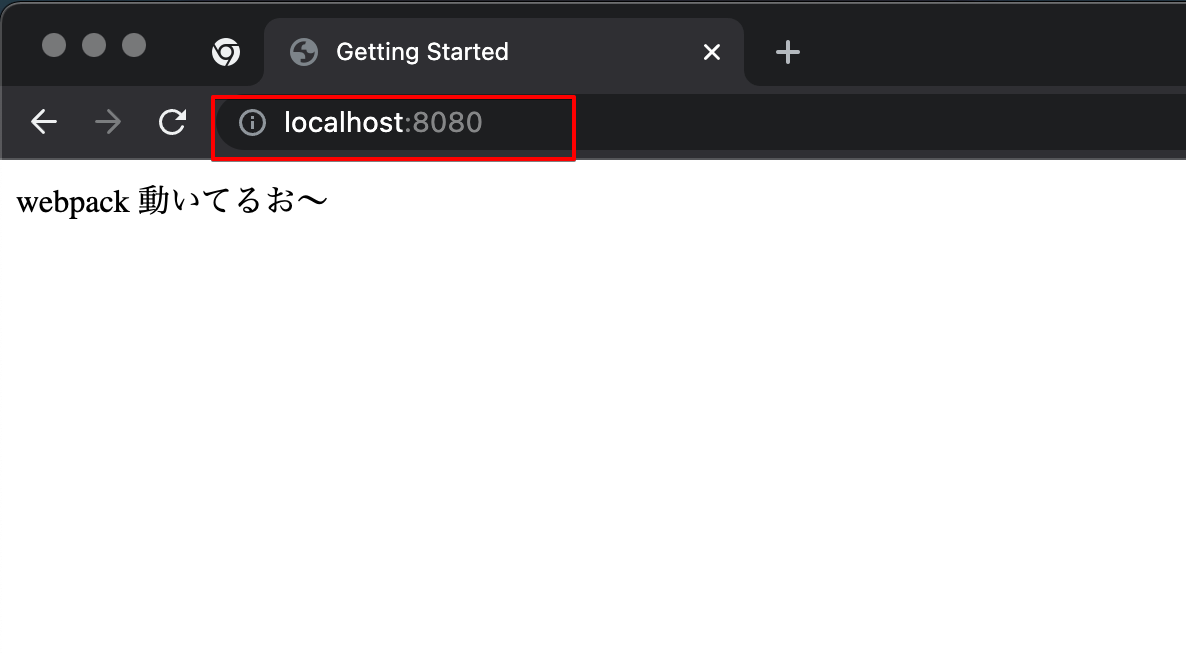
\includegraphics[width=0.8\maxwidth]{./images/02-create-react-app/webpack_test01.png}%
}%
\reviewimagecaption{ブラウザで表示}
\label{image:02-create-react-app:webpack_test01}
\end{reviewimage}

\clearpage


devToolsで「main.js」を確認すると、node\textunderscore{}modulesフォルダ以下にインストールされたJavaScriptが
1つのファイルにまとめられているのが確認できます。

\begin{reviewimage}%%webpack_test02
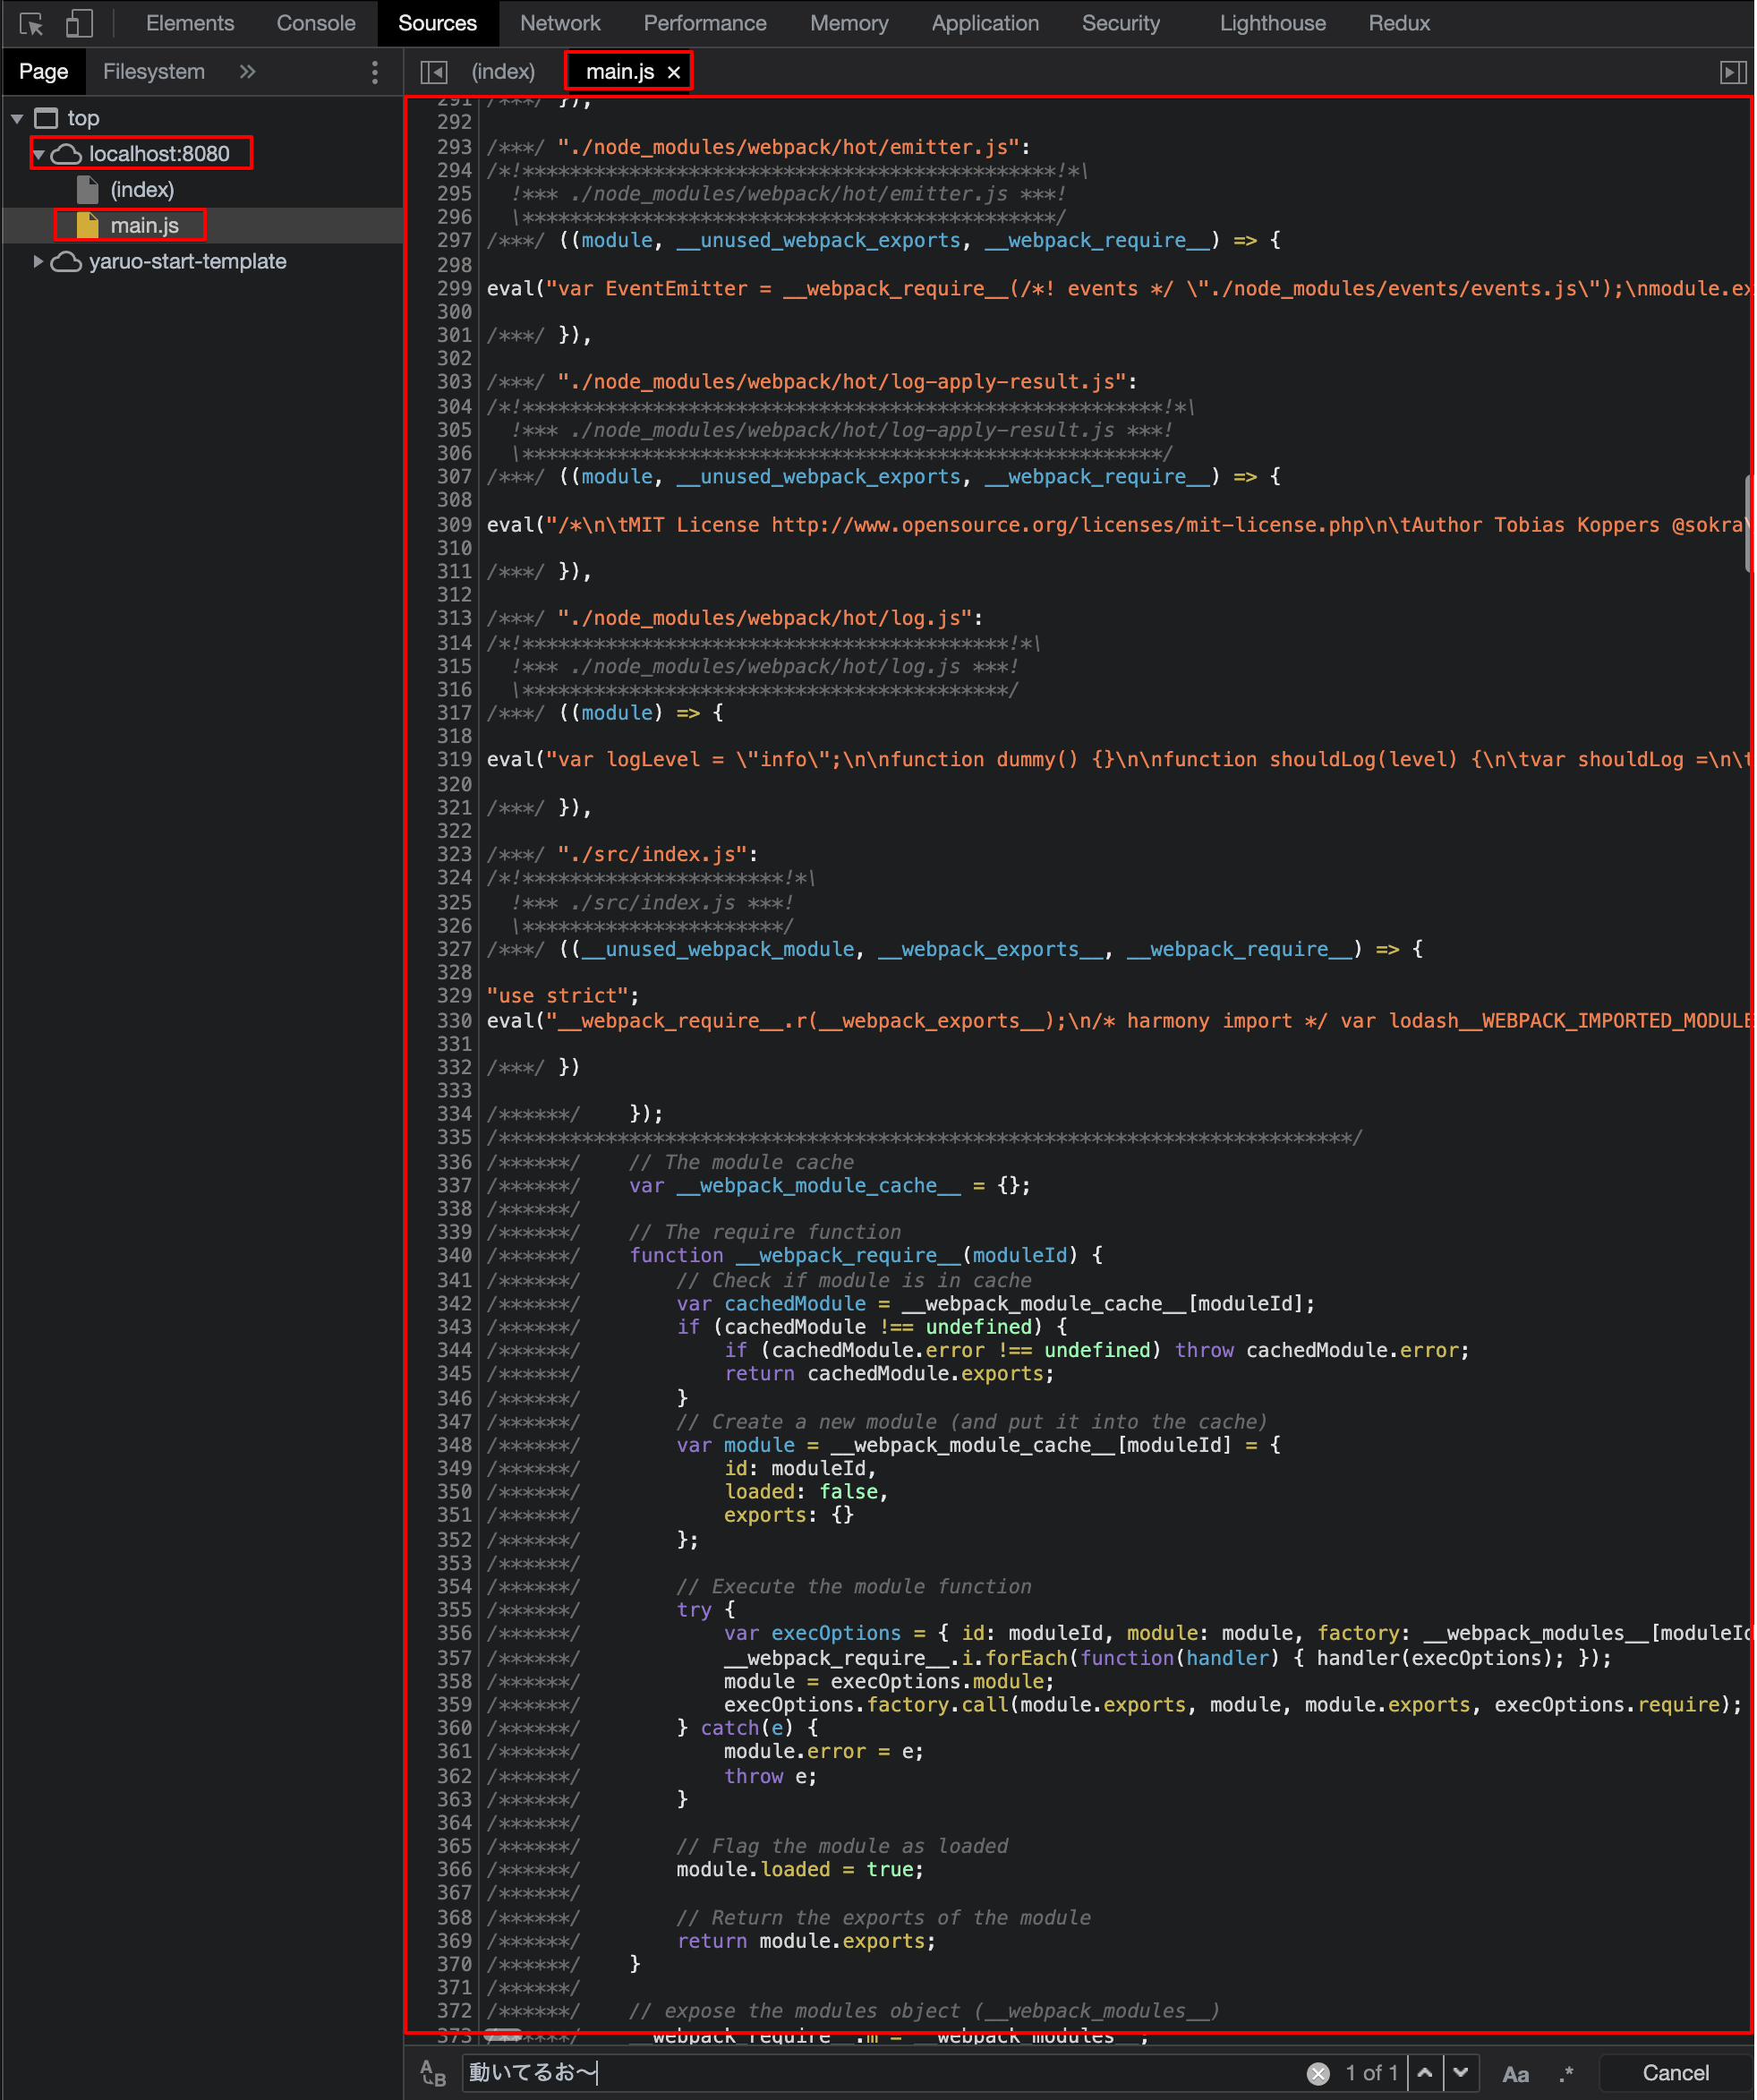
\includegraphics[width=0.8\maxwidth]{./images/02-create-react-app/webpack_test02.png}%
\reviewimagecaption{devToolsでmain.js内を確認}
\label{image:02-create-react-app:webpack_test02}
\end{reviewimage}

\clearpage

\def\startercodeblockfontsize{}
\begin{starterterminal}[]{ビルドの実行}\seqsplit{ \textgreater{} npx webpack build}\end{starterterminal}

上記コマンドを実行すると、distフォルダ以下にmain.jsファイルが出力されます。

\begin{reviewimage}%%webpack_test03
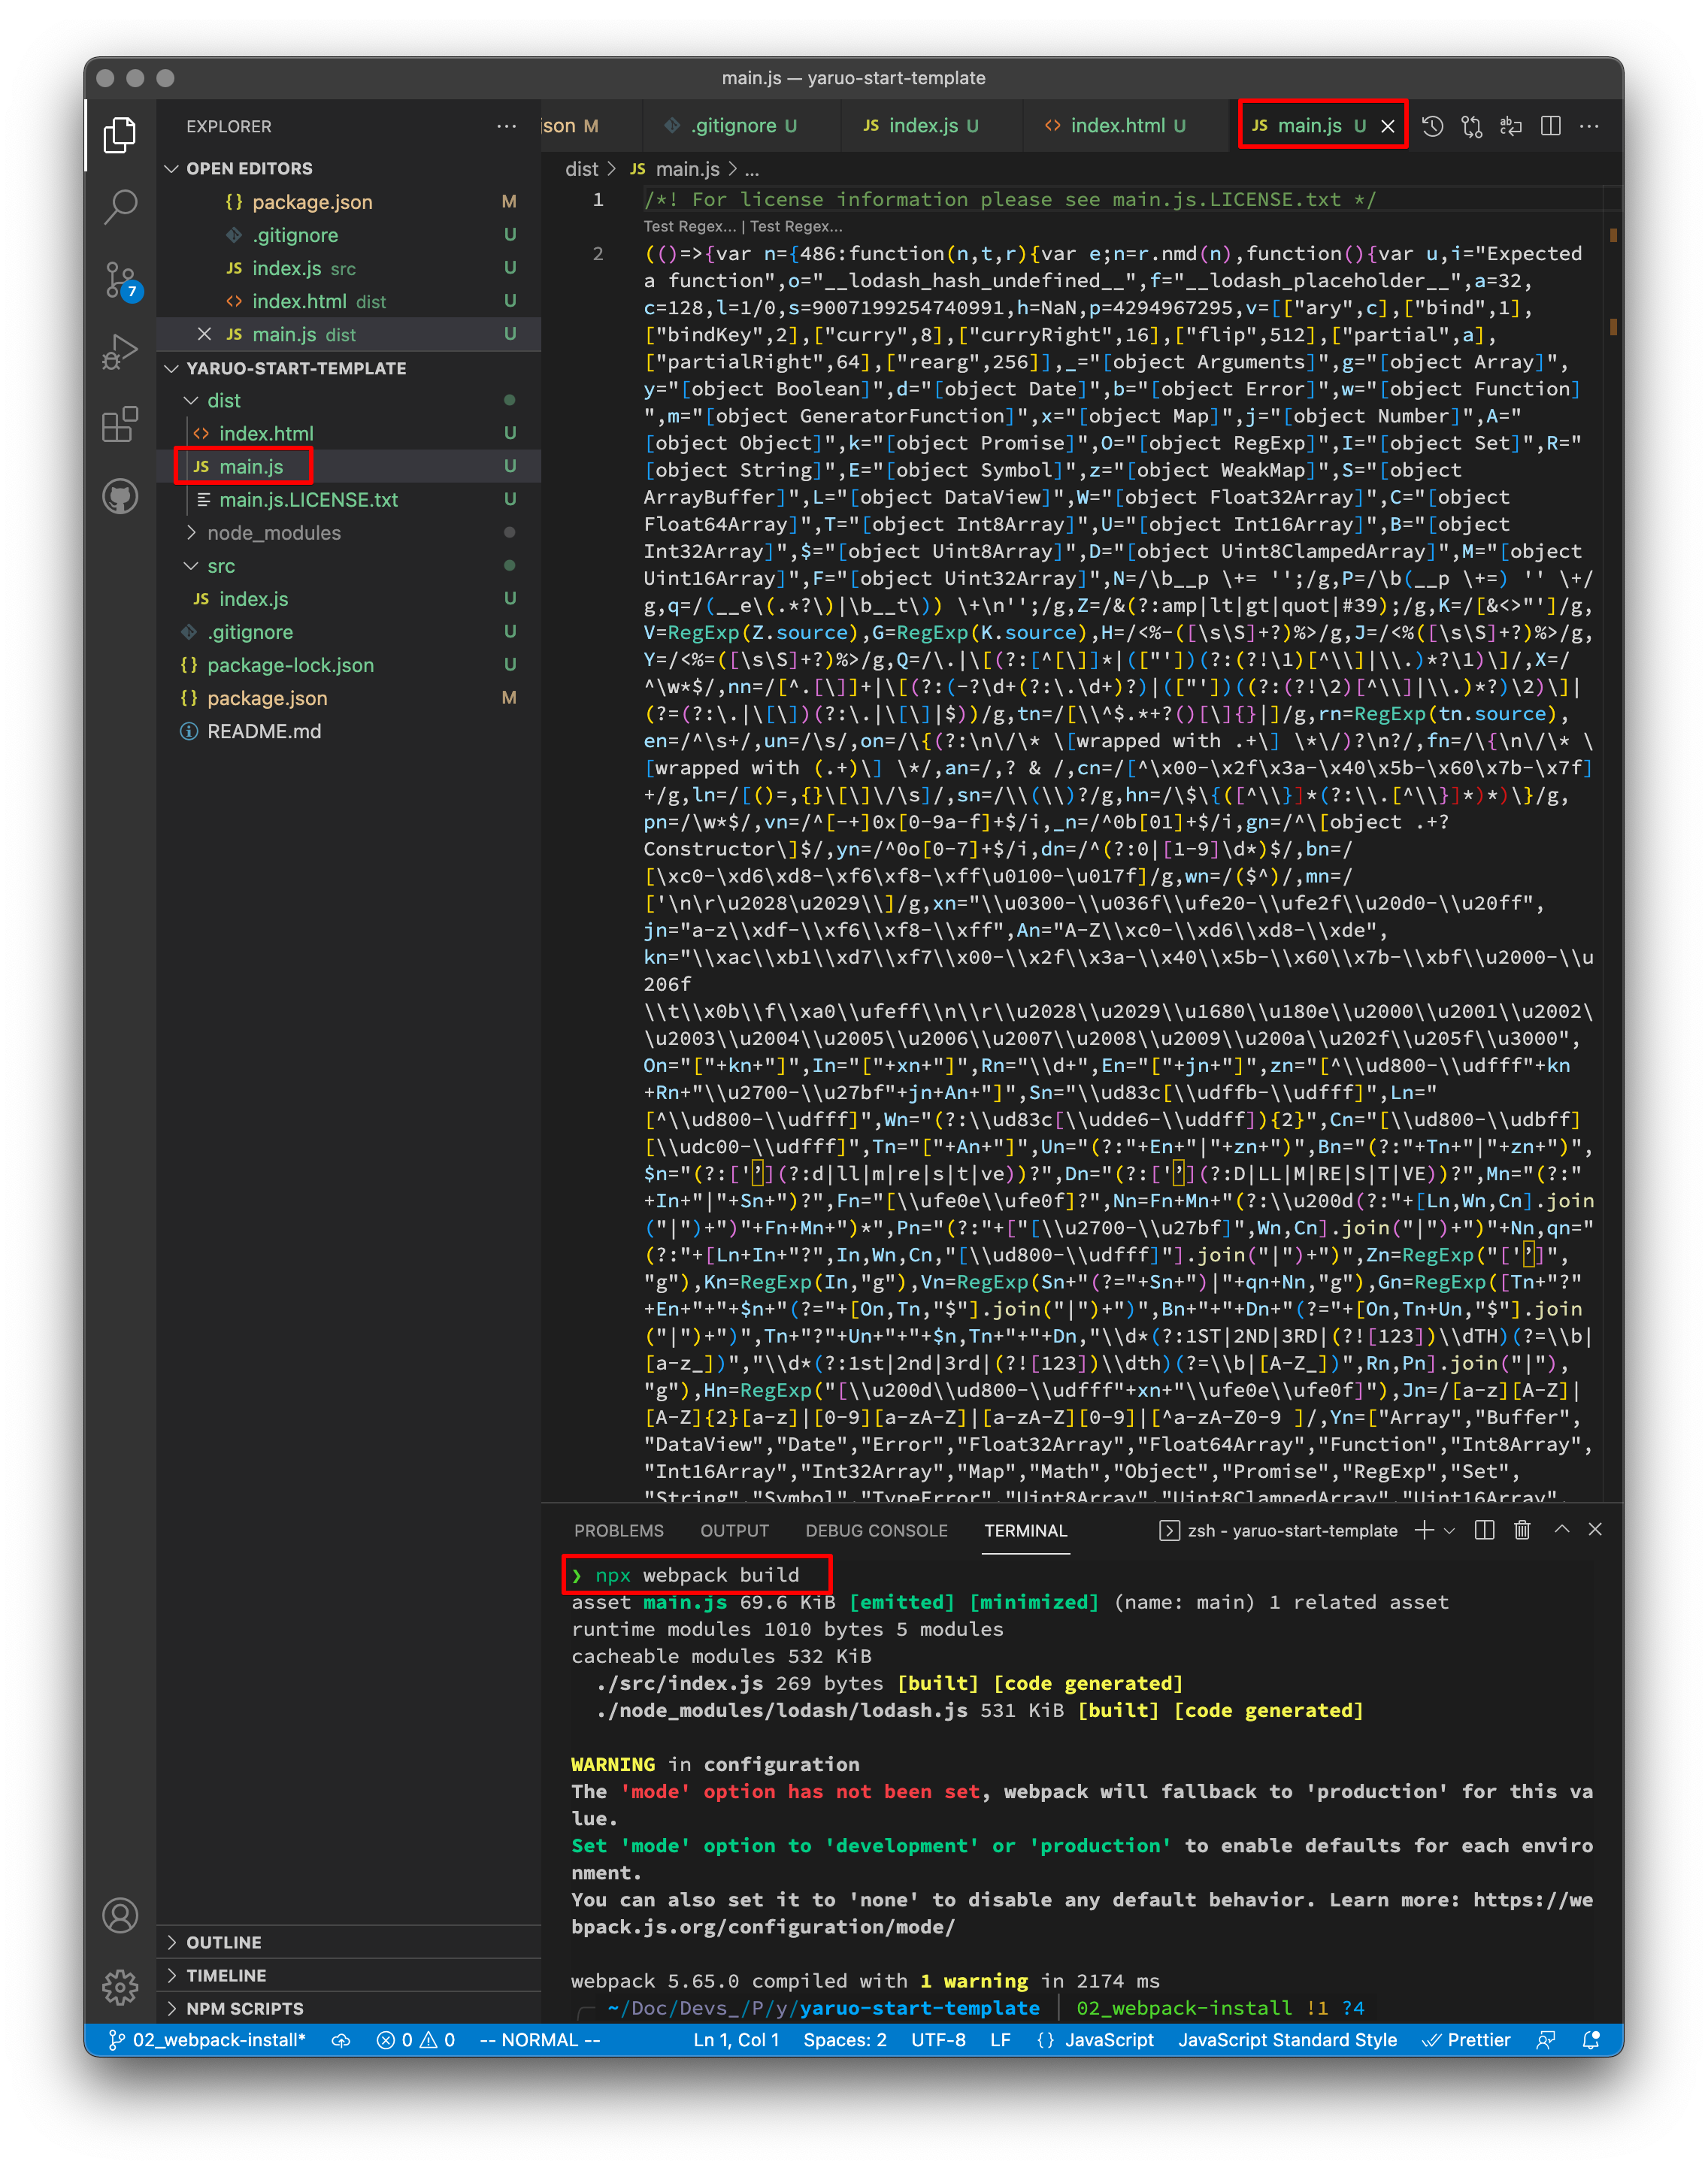
\includegraphics[width=0.8\maxwidth]{./images/02-create-react-app/webpack_test03.png}%
\reviewimagecaption{webpackでビルドしてみた}
\label{image:02-create-react-app:webpack_test03}
\end{reviewimage}

\clearpage

\begin{starternote}[]{}

ここまでの内容は、GitHub上で、以下のコマンドでクローンできます。

\def\startercodeblockfontsize{}
\begin{starterterminal}[]{GitHub}\seqsplit{\textgreater{} git clone {-}b 02\textunderscore{}webpack{-}install https://github.com/yaruo{-}react{-}redux/yaruo{-}start{-}template.git}\end{starterterminal}
\end{starternote}

\clearpage


\subsection{webpackの設定ファイル}
\keeplastskip{
  \label{sec:2-2-4}
  \label{04-webpack-config}
  \par\nobreak
}

自分でwebpack、devServerを動作させてみると、webpackが何をやっているかを理解しやすくなります。

本章では、webpackの設定ファイル「webpack{-}config.js」を作成します。

\vspace*{\baselineskip}

手順は、

\begin{starterenumerate}
\item 「npx webpack{-}cli init」をターミナルで実行し、ひな型を作成。
\item 必要なpluginのインストールと設定ファイルへの追加
\item 不要な設定を削除し、開発時用、製品作成時用でファイルを分ける
\end{starterenumerate}

と、なります。

ターミナルにてコマンドを実行すると、\\[0pt]

\def\startercodeblockfontsize{}
\begin{starterterminal}[]{npx webpack{-}cli initの実行}\seqsplit{ \textgreater{} npx webpack{-}cli init}\end{starterterminal}

このコマンドを実行するには、「@webpack{-}cli/generatorsパッケージが必要ですが、インストールしますか?」と
聞かれますので、エンターキーを押します。

\vspace*{\baselineskip}

@webpack{-}cli/generatorsと依存関係をもつパッケージがインストールされると、設定ファイルを作成するための質問が始まります。
私が選んだ答えと括弧内は表示される選択肢です。

\vspace*{\baselineskip}

\begin{starteritemize}
\item どのタイプのJSを使いますか? {-}{-}\textgreater{} TypeScript(none, ES6)
\item devServerを使いますか? {-}{-}\textgreater{} Yes
\item バンドル用のHTMLファイルを作成しますか? {-}{-}\textgreater{} Yes
\item PWAサポートが必要ですか? {-}{-}\textgreater{} No
\item CSSは、どのタイプを使いますか? {-}{-}\textgreater{} SASS(none, CSS only, LESS, Stylus)
\item SASSと一緒にCSSスタイルも使いますか? {-}{-}\textgreater{} Yes
\item PostCSS(Node.js製のCSSを作るためのフレームワーク)を使いますか? {-}{-}\textgreater{} No
\item ファイル毎にCSSを別にしますか? {-}{-}\textgreater{} Yes
\item 設定ファイルをフォーマットするのにPrettierをインストールしますか? {-}{-}\textgreater{} Yes
\item パッケージマネージャーを選択してください。 {-}{-}\textgreater{} npm
\item package.jsonがすでにありますが上書きしても良いですか? {-}{-}\textgreater{} No
\item README.mdがすでにありますが上書きしても良いですか? {-}{-}\textgreater{} No
\end{starteritemize}

\def\startercodeblockfontsize{}
\begin{starterterminal}[]{webpack{-}config.jsの作成}\seqsplit{  \textgreater{} npx webpack{-}cli init
  [webpack{-}cli] For using this command you need to install: '@webpack{-}cli/generators' package.
  [webpack{-}cli] Would you like to install '@webpack{-}cli/generators' package? (That will run 'npm install {-}D @webpack{-}cli/generators') (Y/n)
  npm WARN deprecated urix@0.1.0: Please see https://github.com/lydell/urix\#deprecated
  npm WARN deprecated resolve{-}url@0.2.1: https://github.com/lydell/resolve{-}url\#deprecated

  added 370 packages, and audited 699 packages in 22s

  58 packages are looking for funding
    run `npm fund` for details

  9 vulnerabilities (4 moderate, 5 high)

  To address all issues (including breaking changes), run:
    npm audit fix {-}{-}force

  Run `npm audit` for details.
  ? Which of the following JS solutions do you want to use? Typescript
  ? Do you want to use webpack{-}dev{-}server? Yes
  ? Do you want to simplify the creation of HTML files for your bundle? Yes
  ? Do you want to add PWA support? No
  ? Which of the following CSS solutions do you want to use? SASS
  ? Will you be using CSS styles along with SASS in your project? Yes
  ? Will you be using PostCSS in your project? No
  ? Do you want to extract CSS for every file? Yes
  ? Do you like to install prettier to format generated configuration? Yes
  ? Pick a package manager: npm
  [webpack{-}cli] ℹ INFO  Initialising project...
   conflict package.json
  ? Overwrite package.json? do not overwrite
       skip package.json
     create src/index.ts
   conflict README.md
  ? Overwrite README.md? do not overwrite
       skip README.md
     create index.html
     create webpack.config.js
     create tsconfig.json

  added 65 packages, and audited 764 packages in 9s

  73 packages are looking for funding
    run `npm fund` for details

  9 vulnerabilities (4 moderate, 5 high)

  To address all issues (including breaking changes), run:
    npm audit fix {-}{-}force

  Run `npm audit` for details.}\end{starterterminal}

質問完了後に必要なパッケージがインストールされ、「webpack.config.js」が作成されます。
また、TypeScript用に「tsconfig.json」も作成されますが、後で作成しますので削除します。

\vspace*{\baselineskip}

作成された「webpack.config.js」を以下のように編集します。

\begin{starteritemize}
\item entry: "./src/index.ts"を"./src/index.js"へ
\item output: path: path.resolve(\textunderscore{}\textunderscore{}dirname, "public")へ
\item distフォルダを削除し、publicフォルダを作成
\end{starteritemize}

\def\startercodeblockfontsize{}
\begin{starterprogram}[]{webpack.config.js}\seqsplit{  // Generated using webpack{-}cli https://github.com/webpack/webpack{-}cli

  const path = require("path");
  const HtmlWebpackPlugin = require("html{-}webpack{-}plugin");
  const MiniCssExtractPlugin = require("mini{-}css{-}extract{-}plugin");

  const isProduction = process.env.NODE\textunderscore{}ENV == "production";

  const stylesHandler = MiniCssExtractPlugin.loader;

  const config = \{
    entry: "./src/index.js", {\reviewballoon{TypeScript導入までは、拡張子jsで}} 
    output: \{
      path: path.resolve(\textunderscore{}\textunderscore{}dirname, "public"), {\reviewballoon{出力フォルダをpublicへ}}
    \},
    devServer: \{
      open: true,
      host: "localhost",
    \},
    plugins: [
      new HtmlWebpackPlugin(\{
        template: "index.html",
      \}),

      new MiniCssExtractPlugin(),

      // Add your plugins here
      // Learn more about plugins from https://webpack.js.org/configuration/plugins/
    ],
    module: \{
      rules: [
        \{
          test: /\reviewbackslash{}.(ts\textbar{}tsx)\textdollar{}/i,
          loader: "ts{-}loader",
          exclude: ["/node\textunderscore{}modules/"],
        \},
        \{
          test: /\reviewbackslash{}.css\textdollar{}/i,
          use: [stylesHandler, "css{-}loader"],
        \},
        \{
          test: /\reviewbackslash{}.s[ac]ss\textdollar{}/i,
          use: [stylesHandler, "css{-}loader", "sass{-}loader"],
        \},
        \{
          test: /\reviewbackslash{}.(eot\textbar{}svg\textbar{}ttf\textbar{}woff\textbar{}woff2\textbar{}png\textbar{}jpg\textbar{}gif)\textdollar{}/i,
          type: "asset",
        \},

        // Add your rules for custom modules here
        // Learn more about loaders from https://webpack.js.org/loaders/
      ],
    \},
    resolve: \{
      extensions: [".tsx", ".ts", ".js"],
    \},
  \};

  module.exports = () =\textgreater{} \{
    if (isProduction) \{
      config.mode = "production";
    \} else \{
      config.mode = "development";
    \}
    return config;
  \};
}\end{starterprogram}

{\reviewstrong{プラグインのインストール}}\\[0pt]
追加で、以下のプラグイン、ローダも追加します。

\begin{starteritemize}
\item uglify{-}js プロダクション出力時にconsole関数を除去
\item terser{-}webpack{-}plugin 上記をwebpackで使用する場合必要
\item css{-}minimizer{-}webpack{-}plugin CSSをminimize
\item webpack{-}merge 複数のwebpack{-}configファイルをマージする
\end{starteritemize}

ターミナルで以下のコマンドを実行します。

\def\startercodeblockfontsize{}
\begin{starterterminal}[]{追加プラグイン、ローダのインストール}\seqsplit{ \textgreater{} npm install {-}D uglify{-}js terser{-}webpack{-}plugin css{-}minimizer{-}webpack{-}plugin webpack{-}merge}\end{starterterminal}

追加のプラグイン、ローダの設定を追加したwebpack.config.jsです。devServerでページを表示する際に、
デフォルトのブラウザではなくdevToolsの強力な「Google Chrome」を使うようにしました。

\vspace*{\baselineskip}

OS毎にChromeのアプリケーション名が違うためOSを取得し対応した「Chrome名」に変換するためのswitch文を追加しています。
「create{-}react{-}app」だと、結構複雑なことをやってGoogle Chromeを起動しています。

\vspace*{\baselineskip}

興味のある方は、「create{-}react{-}app」を使ってプロジェクト作成し、react{-}scriptsを追うとお勉強になります。

\def\startercodeblockfontsize{}
\begin{starterprogram}[]{webpack.config.js}\seqsplit{  // Generated using webpack{-}cli https://github.com/webpack/webpack{-}cli
  const path = require('path');
  const HtmlWebpackPlugin = require('html{-}webpack{-}plugin');
  const MiniCssExtractPlugin = require('mini{-}css{-}extract{-}plugin');
  const TerserPlugin = require('terser{-}webpack{-}plugin');
  const CssMinimizerPlugin = require('css{-}minimizer{-}webpack{-}plugin');
  const os = require('os');

  const isProduction = process.env.NODE\textunderscore{}ENV == 'production';

  const stylesHandler = MiniCssExtractPlugin.loader;

  let devBrowser = 'Google Chrome';
  switch (os.platform()) \{
    case 'win32':
      devBrowser = 'chrome';
      break;
    case 'linux':
      devBrowser = 'google{-}chrome';
    default:
      break;
  \}

  const config = \{
    entry: './src/index.js',
    output: \{
      path: path.resolve(\textunderscore{}\textunderscore{}dirname, 'public'),
      assetModuleFilename: 'images/[name][ext][query]',
      clean: true,
    \},
    plugins: [
      new HtmlWebpackPlugin(\{
        template: 'index.html',
      \}),

      new MiniCssExtractPlugin(),

      // Add your plugins here
      // Learn more about plugins from https://webpack.js.org/configuration/plugins/
      new CssMinimizerPlugin(),
    ],
    module: \{
      rules: [
        \{
          test: /\reviewbackslash{}.(ts\textbar{}tsx)\textdollar{}/i,
          loader: 'ts{-}loader',
          exclude: ['/node\textunderscore{}modules/'],
        \},
        \{
          test: /\reviewbackslash{}.css\textdollar{}/i,
          use: [stylesHandler, 'css{-}loader'],
        \},
        \{
          test: /\reviewbackslash{}.s[ac]ss\textdollar{}/i,
          use: [stylesHandler, 'css{-}loader', 'sass{-}loader'],
        \},
        \{
          test: /\reviewbackslash{}.(eot\textbar{}svg\textbar{}ttf\textbar{}woff\textbar{}woff2\textbar{}png\textbar{}jpg\textbar{}gif)\textdollar{}/i,
          type: 'asset',
        \},

        // Add your rules for custom modules here
        // Learn more about loaders from https://webpack.js.org/loaders/
      ],
    \},
    resolve: \{
      extensions: ['.tsx', '.ts', '.js'],
    \},
    optimization: \{
      minimize: true,
      minimizer: [
        new TerserPlugin(\{
          minify: TerserPlugin.uglifyJsMinify,
          terserOptions: \{
            compress: \{
              drop\textunderscore{}console: true,
            \},
          \},
        \}),
        new CssMinimizerPlugin(),
      ],
    \},
    devtool: 'eval{-}source{-}map',
    devServer: \{
      open: \{
        app: \{
          name: devBrowser,
        \},
      \},
      host: 'localhost',
      port: 3000,
      static: './public',
    \},
  \};

  module.exports = () =\textgreater{} \{
    if (isProduction) \{
      config.mode = 'production';
    \} else \{
      config.mode = 'development';
    \}
    return config;
  \};
}\end{starterprogram}

動作確認のために「index.js」を書き換えます。いつの間にかプロジェクトフォルダ直下に「index.html」も
作成されています。

\vspace*{\baselineskip}

「index.js」に、動作確認用に追加するスタイル指定用の「sytle.css」、「style.scss」も追加します。

\def\startercodeblockfontsize{}
\begin{starterprogram}[]{style.css}\seqsplit{  div \{
    background{-}color: aqua;
  \}}\end{starterprogram}
\def\startercodeblockfontsize{}
\begin{starterprogram}[]{style.scss}\seqsplit{  \textdollar{}primary{-}color: \#f00;

  div \{
    color: \textdollar{}primary{-}color;
  \}}\end{starterprogram}
\vspace*{\baselineskip}

適当な画像ファイルを用意し、「src/assets/images」フォルダを作成し追加します。

\vspace*{\baselineskip}

コマンドを「package.json」に、スクリプトとして追加します。

\def\startercodeblockfontsize{}
\begin{starterprogram}[]{package.jsonのスクリプト部分}\seqsplit{  "scripts": \{
    "test": "echo \reviewbackslash{}"Error: no test specified\reviewbackslash{}" \&\& exit 1",
    "build": "webpack {-}{-}mode=production",
    "build:dev": "webpack {-}{-}mode=development",
    "build:prod": "webpack {-}{-}mode=production",
    "start": "webpack serve"
  \},}\end{starterprogram}

まずは、ファイルを出力しないでブラウザで表示します。

\def\startercodeblockfontsize{}
\begin{starterterminal}[]{ブラウザで表示}\seqsplit{ \textgreater{} npm run start}\end{starterterminal}

「div」要素の背景、文字色も「style.css」、「style.scss」から作成された「main.css」から反映されています。
また、「index.html」には、作成された「main.js」、「main.css」を読み込む部分はありませんが、
webpackが「HtmlWebpackPlugin」で自動で読込部分が追加されています。

\begin{reviewimage}%%webpack_test04
\starterimageframe{%
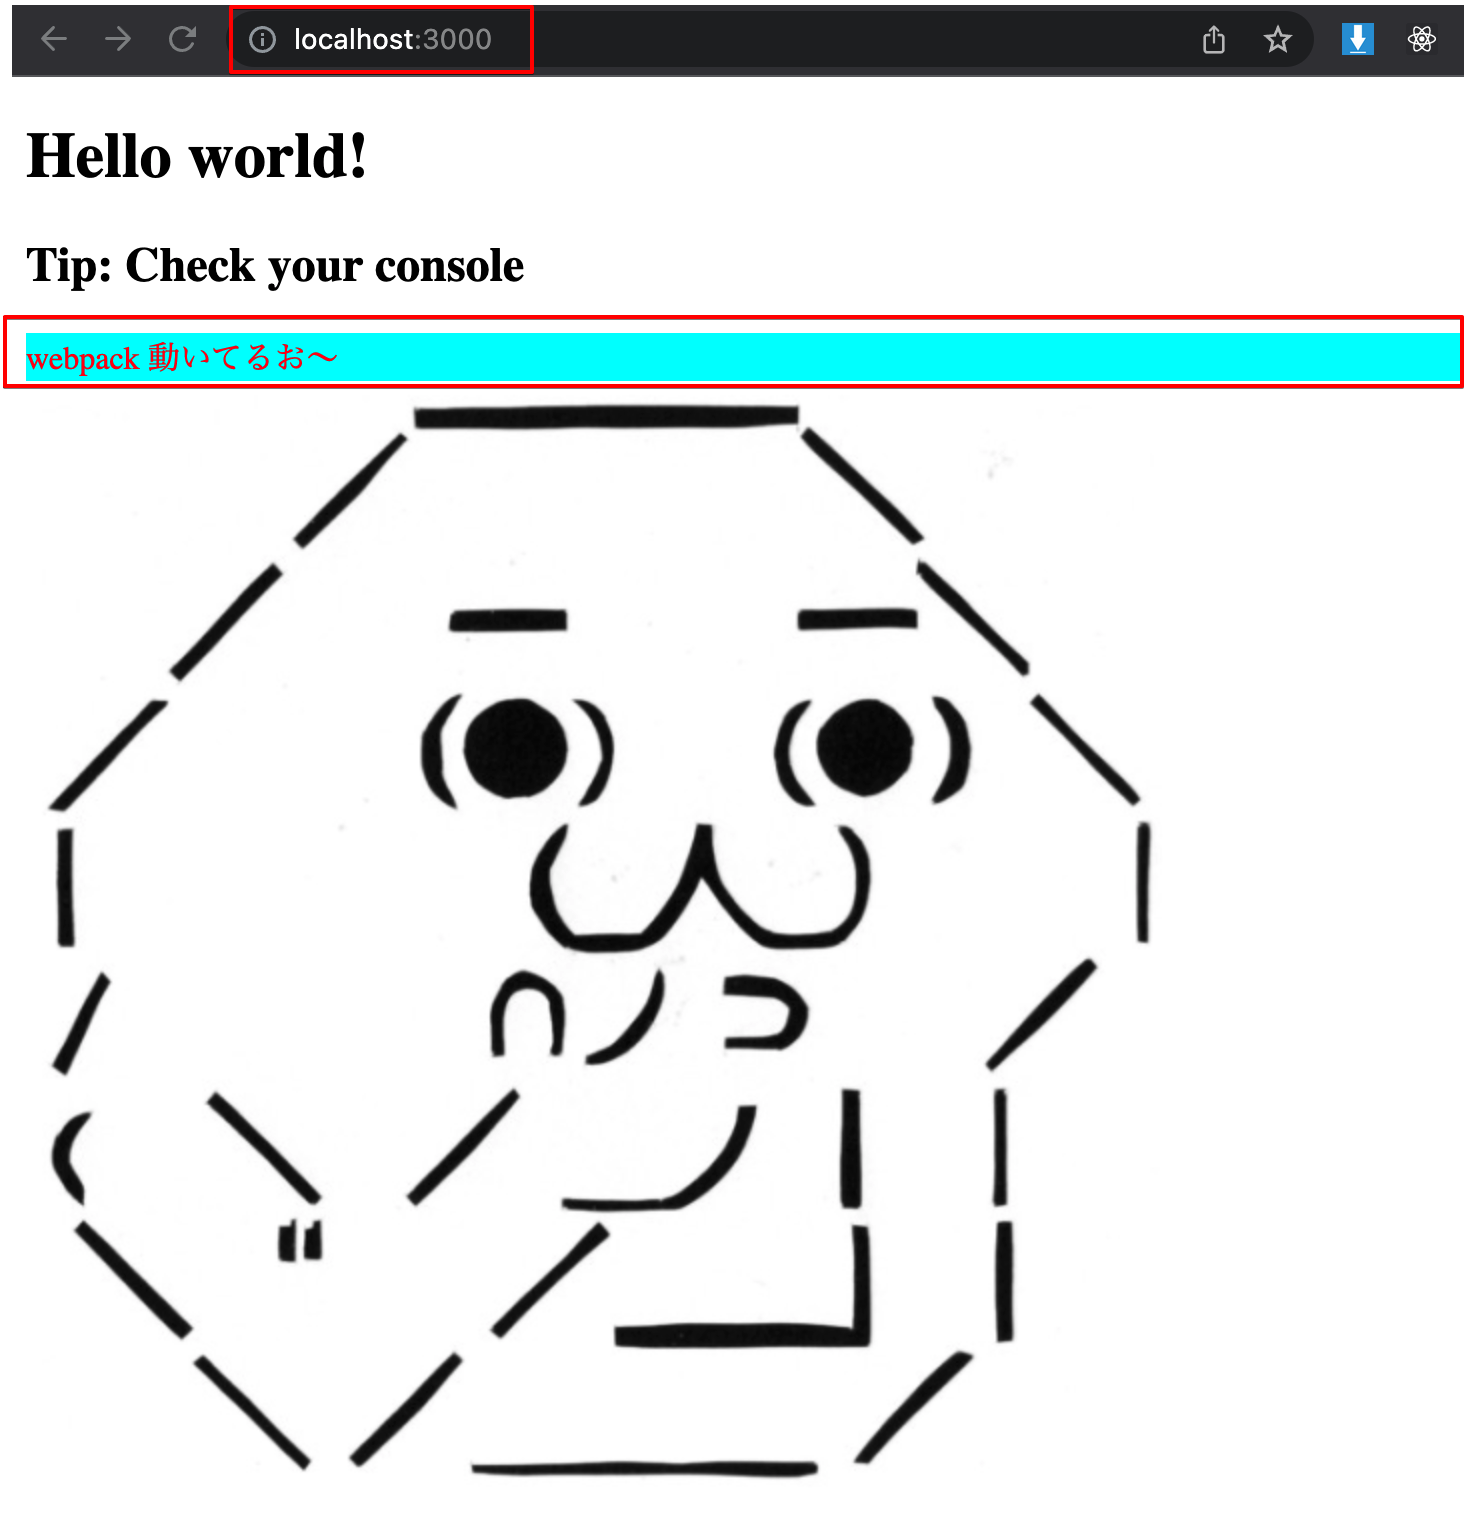
\includegraphics[width=0.7\maxwidth]{./images/02-create-react-app/webpack_test04.png}%
}%
\reviewimagecaption{desc}
\label{image:02-create-react-app:webpack_test04}
\end{reviewimage}

\clearpage


次にプロダクション用にビルドしてみます。

\def\startercodeblockfontsize{}
\begin{starterterminal}[]{ビルド}\seqsplit{ \textgreater{} npm run build}\end{starterterminal}

下図のように、\\[0pt]

\begin{starteritemize}
\item index.html
\item main.js
\item main.css
\item images/画像ファイル
\end{starteritemize}

が出力されていますので、ファイル開き内容を確認してください。

\begin{reviewimage}%%webpack_test05
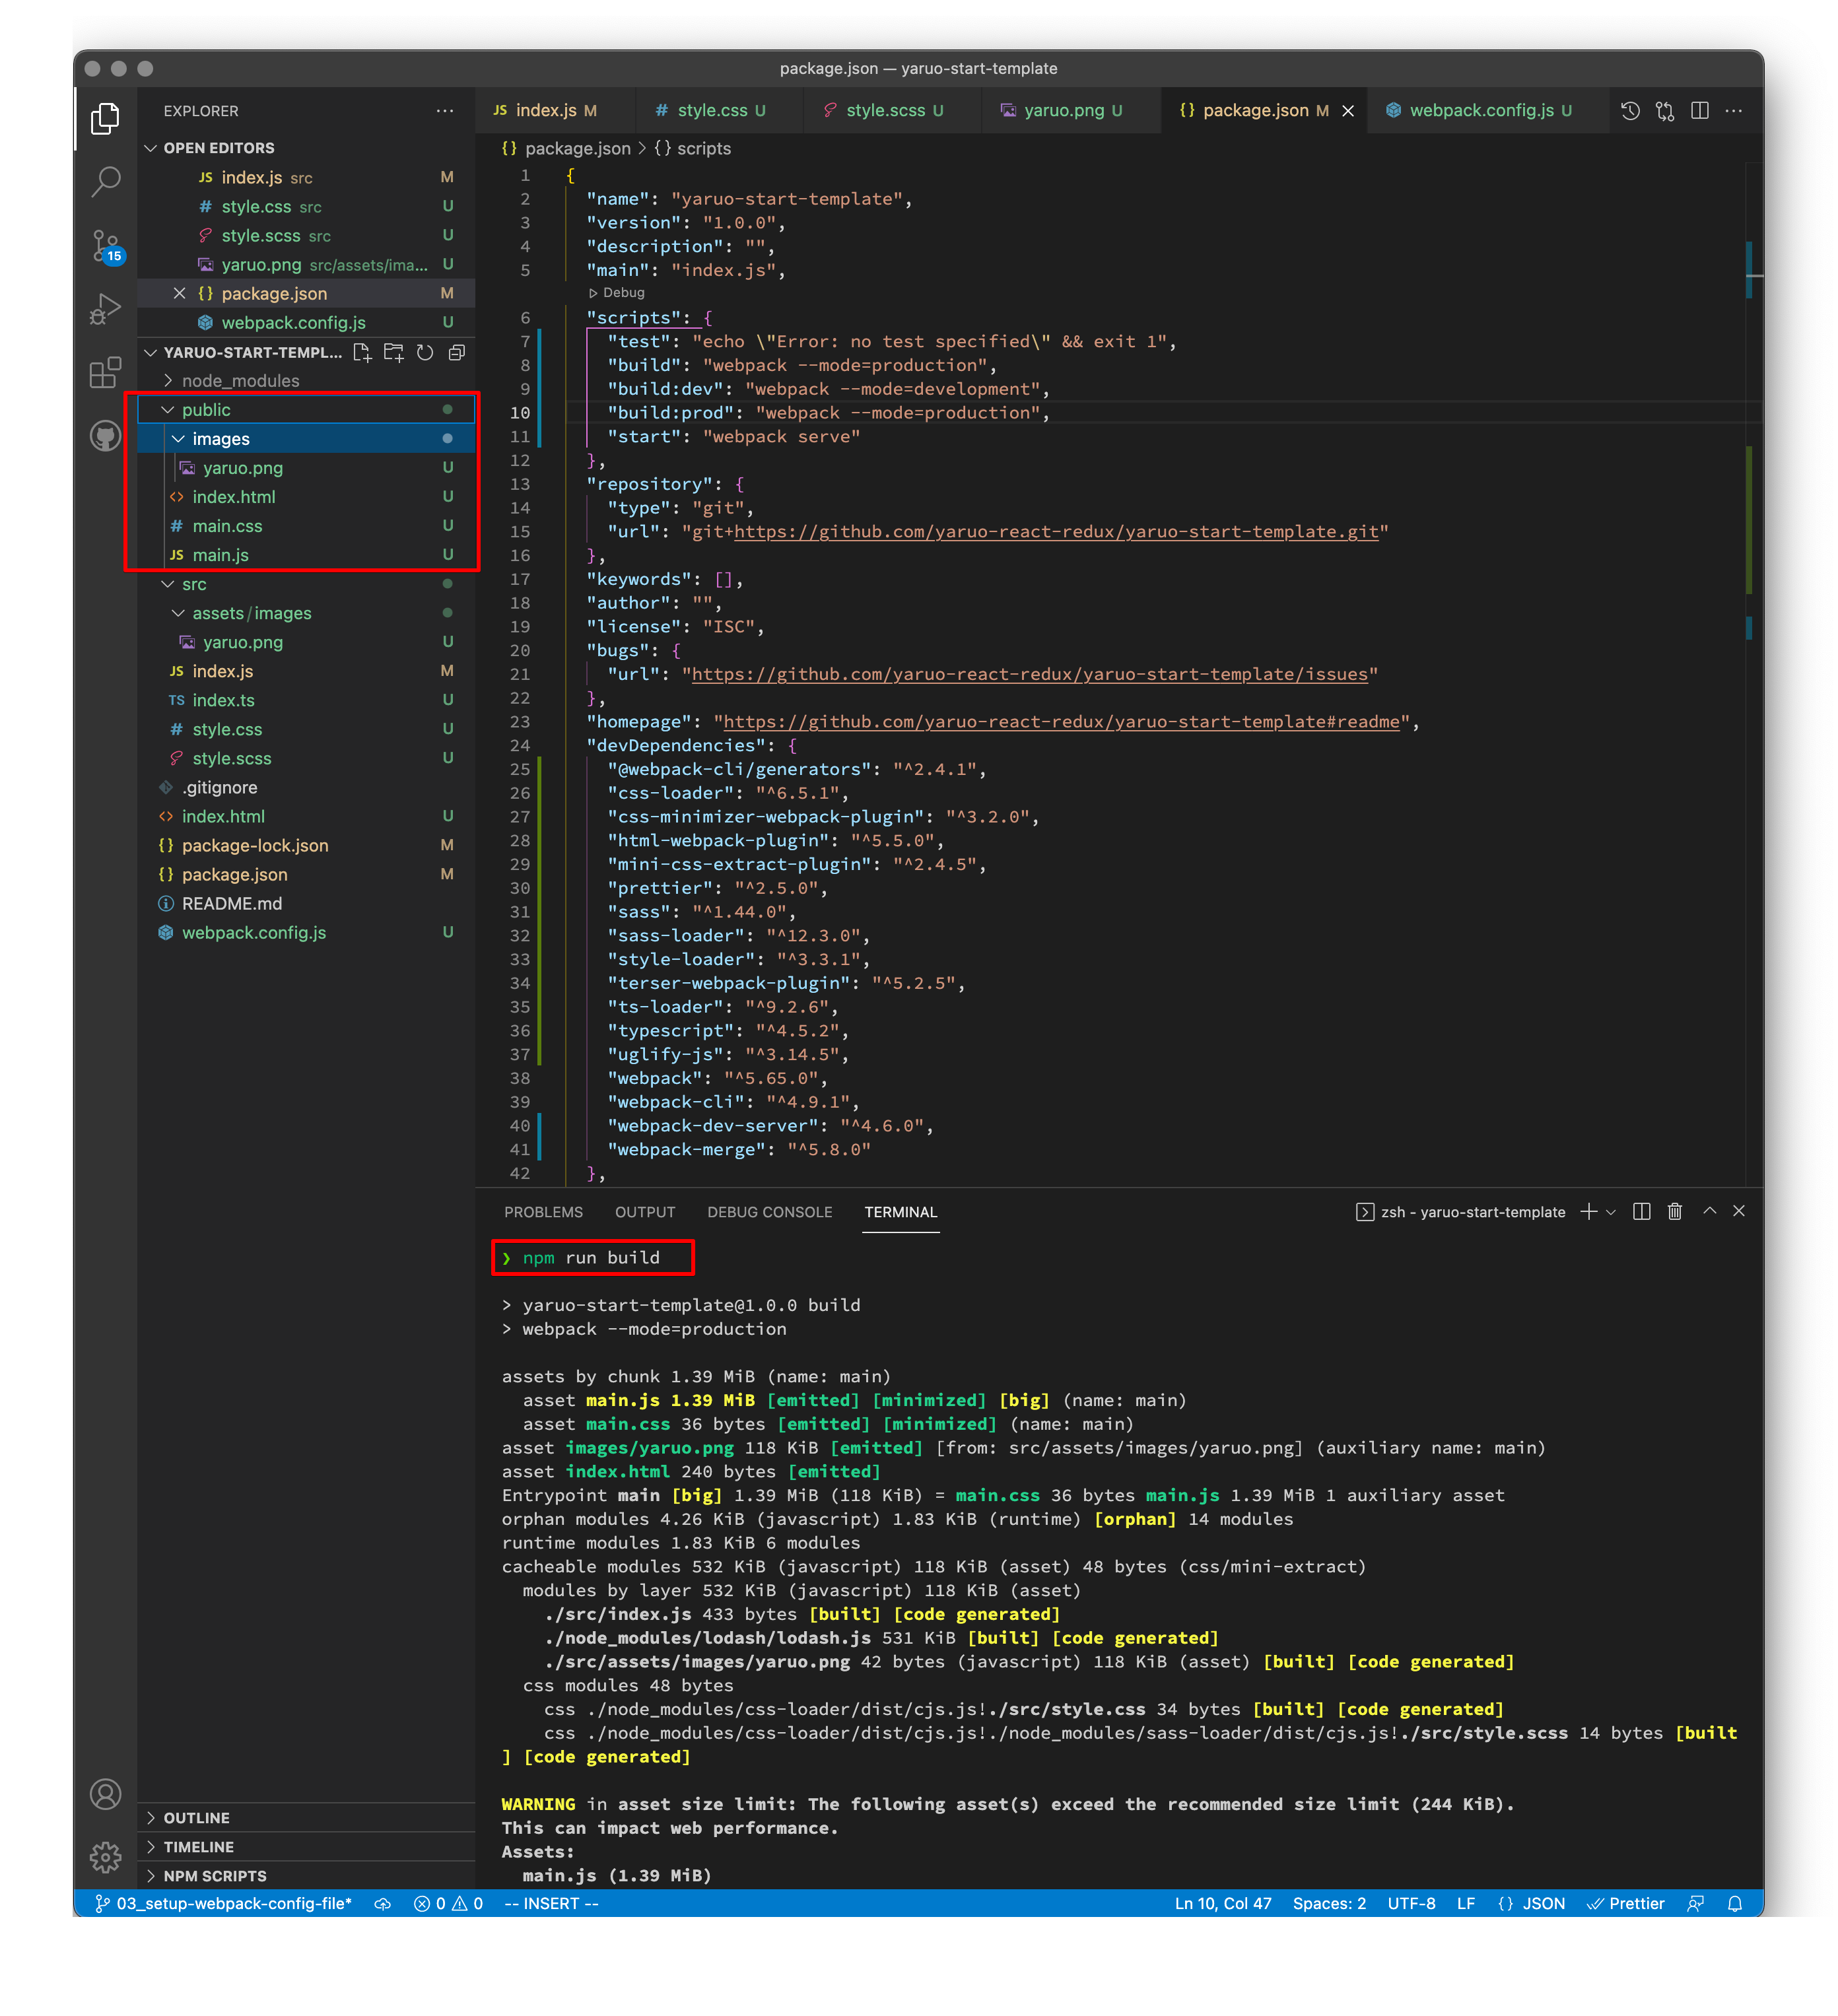
\includegraphics[width=1.0\maxwidth]{./images/02-create-react-app/webpack_test05.png}%
\label{image:02-create-react-app:webpack_test05}
\end{reviewimage}

\clearpage

\begin{starternote}[]{}

ここまでの内容は、GitHub上で、以下のコマンドでクローンできます。

\def\startercodeblockfontsize{}
\begin{starterterminal}[]{GitHub}\seqsplit{\textgreater{} git clone {-}b 03\textunderscore{}setup{-}webpack{-}config{-}file https://github.com/yaruo{-}react{-}redux/yaruo{-}start{-}template.git}\end{starterterminal}
\end{starternote}

\subsection{webpack設定ファイルを分割する}
\keeplastskip{
  \label{sec:2-2-5}
  \label{sec-04-webpack-config-all}
  \par\nobreak
}

問題なく動作した「webpack.config.js」ですが、今後の運用を考え「開発用」、「プロダクション用」、「共通分」に切り分けます。
devServer関連はプロダクションには関係ありませんし、minimizer関連は開発時には邪魔です。

本家でも推奨\footnote{\url{https://webpack.js.org/guides/production/}}されています。

\vspace*{\baselineskip}

「webpack.config.js」を以下のよう分割し、共用部分は「webpack{-}merge」を使用して統合します。

\begin{starteritemize}
\item 共用 webpack.common.js
\item 開発用 webpack.dev.js
\item プロダクション用 webpack.prod.js
\end{starteritemize}

開発用はdevServer関係、プロダクション用はminimizer関係、それ以外は共用として分けていきます。

\vspace*{\baselineskip}

「webpack.dev.js」を作成し、「webpack.config.js」全体を貼り付けdevServer、debtoolを
残し、「module」はCSS関係のみで「style{-}loader」を使うように変更します。

\vspace*{\baselineskip}

また、「mode:'development'」を追加します。

\def\startercodeblockfontsize{}
\begin{starterprogram}[]{webpack.dev.js}\seqsplit{  const \{ merge \} = require('webpack{-}merge');
  const common = require('./webpack.common');
  const os = require('os');

  let devBrowser = 'Google Chrome';
  switch (os.platform()) \{
    case 'win32':
      devBrowser = 'chrome';
      break;
    case 'linux':
      devBrowser = 'google{-}chrome';
      break;
    default:
      break;
  \}

  module.exports = merge(common, \{
    mode: 'development',
    module: \{
      rules: [
        \{
          test: /\reviewbackslash{}.css\textdollar{}/i,
          use: ['style{-}loader', 'css{-}loader'],
        \},
        \{
          test: /\reviewbackslash{}.s[ac]ss\textdollar{}/i,
          use: ['style{-}loader', 'css{-}loader', 'sass{-}loader'],
        \},
      ],
    \},
    devtool: 'eval{-}source{-}map',
    devServer: \{
      open: \{
        app: \{
          name: devBrowser,
        \},
      \},
      host: 'localhost',
      port: 3000,
      static: './public',
    \},
  \});
}\end{starterprogram}

プロダクション用も、「webpack.config.js」全体を貼り付け、CssMinimizer関連を中心に「module」はCSSの抽出のままで
不要な部分を削除します。

\vspace*{\baselineskip}

こちらは、「mode:'production'」を追加します。

\def\startercodeblockfontsize{}
\begin{starterprogram}[]{webpack.prod.js}\seqsplit{  const \{ merge \} = require('webpack{-}merge');
  const common = require('./webpack.common');
  const MiniCssExtractPlugin = require('mini{-}css{-}extract{-}plugin');
  const TerserPlugin = require('terser{-}webpack{-}plugin');
  const CssMinimizerPlugin = require('css{-}minimizer{-}webpack{-}plugin');

  module.exports = merge(common, \{
    mode: 'production',
    plugins: [new MiniCssExtractPlugin(), new CssMinimizerPlugin()],
    module: \{
      rules: [
        \{
          test: /\reviewbackslash{}.css\textdollar{}/i,
          use: [MiniCssExtractPlugin.loader, 'css{-}loader'],
        \},
        \{
          test: /\reviewbackslash{}.s[ac]ss\textdollar{}/i,
          use: [MiniCssExtractPlugin.loader, 'css{-}loader', 'sass{-}loader'],
        \},
      ],
    \},
    resolve: \{
      extensions: ['.tsx', '.ts', '.js'],
    \},
    optimization: \{
      minimize: true,
      minimizer: [
        new TerserPlugin(\{
          minify: TerserPlugin.uglifyJsMinify,
          terserOptions: \{
            compress: \{
              drop\textunderscore{}console: true,
            \},
          \},
        \}),
        new CssMinimizerPlugin(),
      ],
    \},
  \});}\end{starterprogram}

共通部分も、「webpack.config.js」全体を貼り付け、上記ファイルにあるものを削除します。

\def\startercodeblockfontsize{}
\begin{starterprogram}[]{webpack.common.js}\seqsplit{  const path = require('path');
  const HtmlWebpackPlugin = require('html{-}webpack{-}plugin');

  module.exports = \{
    entry: './src/index.js',
    output: \{
      path: path.resolve(\textunderscore{}\textunderscore{}dirname, 'public'),
      assetModuleFilename: 'images/[name][ext][query]',
      clean: true,
    \},
    plugins: [
      new HtmlWebpackPlugin(\{
        template: 'index.html',
      \}),
    ],
    module: \{
      rules: [
        \{
          test: /\reviewbackslash{}.(ts\textbar{}tsx)\textdollar{}/i,
          loader: 'ts{-}loader',
          exclude: ['/node\textunderscore{}modules/'],
        \},
        \{
          test: /\reviewbackslash{}.(eot\textbar{}svg\textbar{}ttf\textbar{}woff\textbar{}woff2\textbar{}png\textbar{}jpg\textbar{}gif)\textdollar{}/i,
          type: 'asset',
        \},
      ],
    \},
    resolve: \{
      extensions: ['.tsx', '.ts', '.js'],
    \},
  \};
}\end{starterprogram}

webpackの設定ファイル名がデフォルトから変更になったので、「package.json」のスクリプト部分を変更します。

\def\startercodeblockfontsize{}
\begin{starterprogram}[]{package.jsonのスクリプト部分}\seqsplit{  "scripts": \{
    "test": "echo \reviewbackslash{}"Error: no test specified\reviewbackslash{}" \&\& exit 1",
    "build": "webpack {-}{-}config webpack.prod.js",
    "build:dev": "webpack {-}{-}config webpack.dev.js",
    "build:prod": "webpack {-}{-}config webpack.prod.js",
    "start": "webpack serve {-}{-}config webpack.dev.js"
  \},}\end{starterprogram}

ターミナル上で、「npm run start」、「npm run build」で動作確認を行います。

\begin{starternote}[]{}

ここまでの内容は、GitHub上で、以下のコマンドでクローンできます。

\def\startercodeblockfontsize{}
\begin{starterterminal}[]{GitHub}\seqsplit{\textgreater{} git clone {-}b 04\textunderscore{}webpack{-}config{-}split https://github.com/yaruo{-}react{-}redux/yaruo{-}start{-}template.git}\end{starterterminal}
\end{starternote}

\subsection{Babel.jsのインストールと設定}
\keeplastskip{
  \label{sec:2-2-6}
  \label{sec04-babeljs}
  \par\nobreak
}

Babel.jsとは、Babel.jsのトップページの例にあるように、
モダンJS(ES2015移行のJavaScript)を未対応の古いブラウザでも解釈できるようなJavaScriptに変換してくれるトランスコンパイラ(変換器)です。

\begin{reviewimage}%%babel01
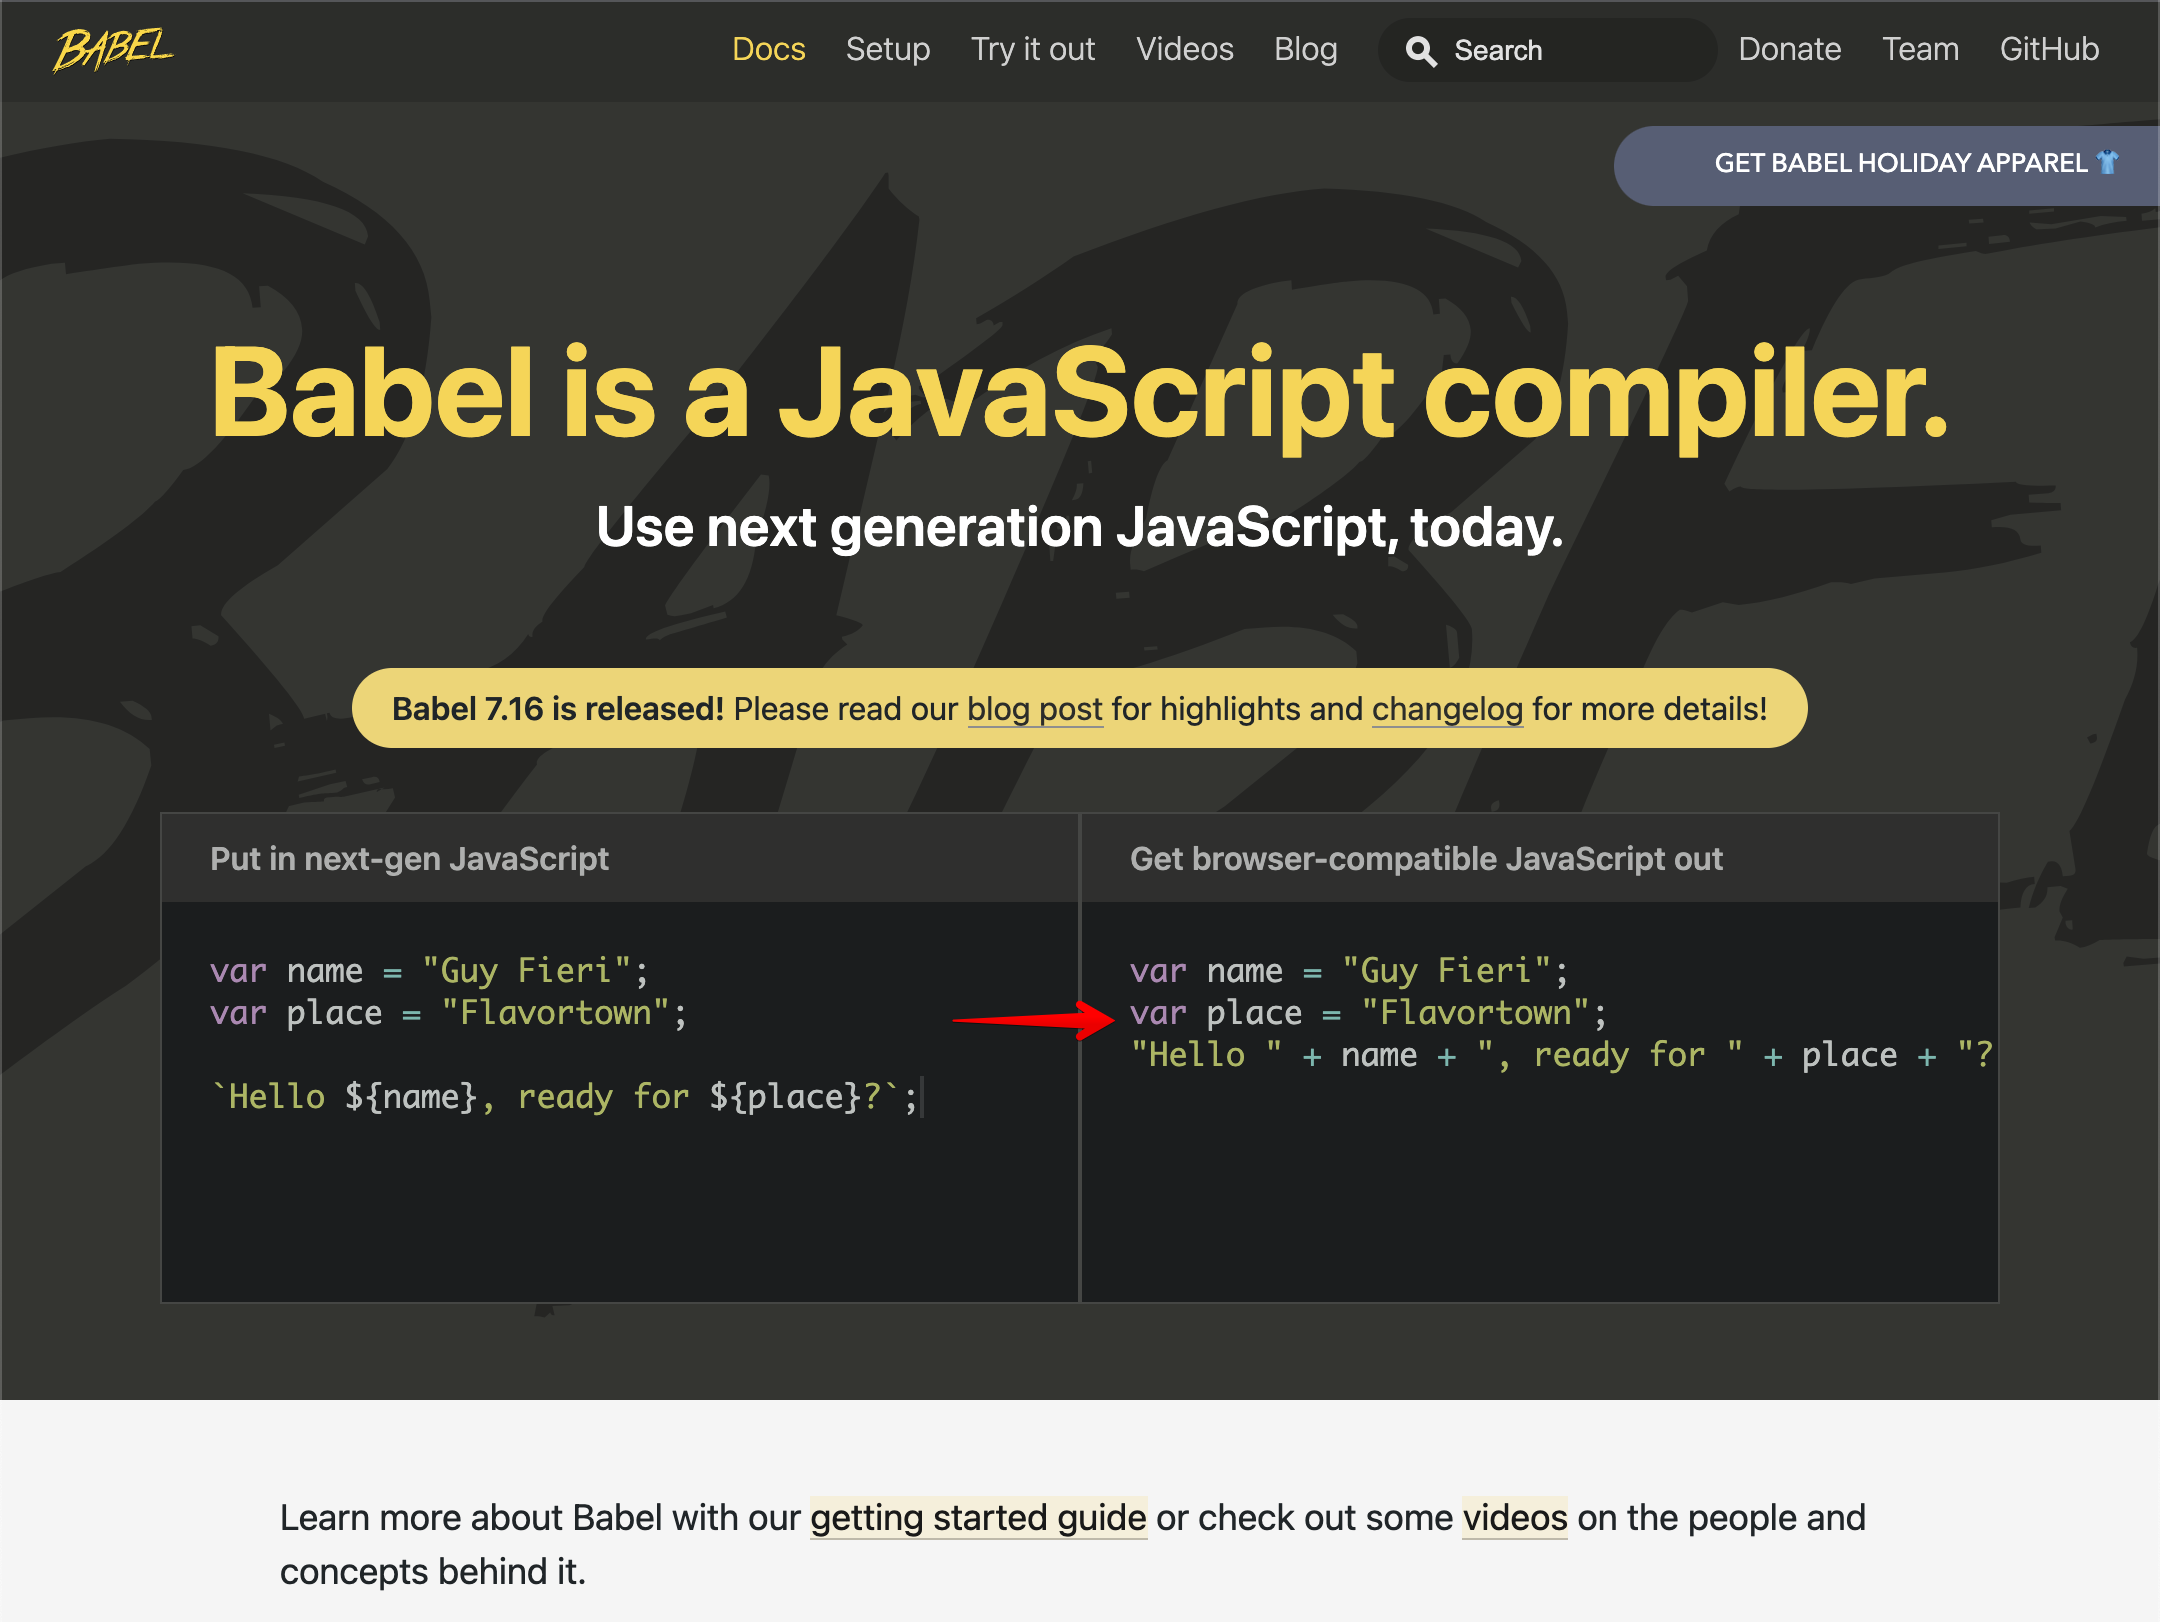
\includegraphics[width=1.0\maxwidth]{./images/02-create-react-app/babel01.png}%
\reviewimagecaption{Babel.js本家ページ}
\label{image:02-create-react-app:babel01}
\end{reviewimage}

それでは、プロジェクトに「Babel.js」を導入していきます。

\vspace*{\baselineskip}

Babel.jsのトップページの上部にあるメニューの「Setup」をクリックします。すると、手順に従うように番号のついた案内ページが表示されます。

\begin{reviewimage}%%babel02
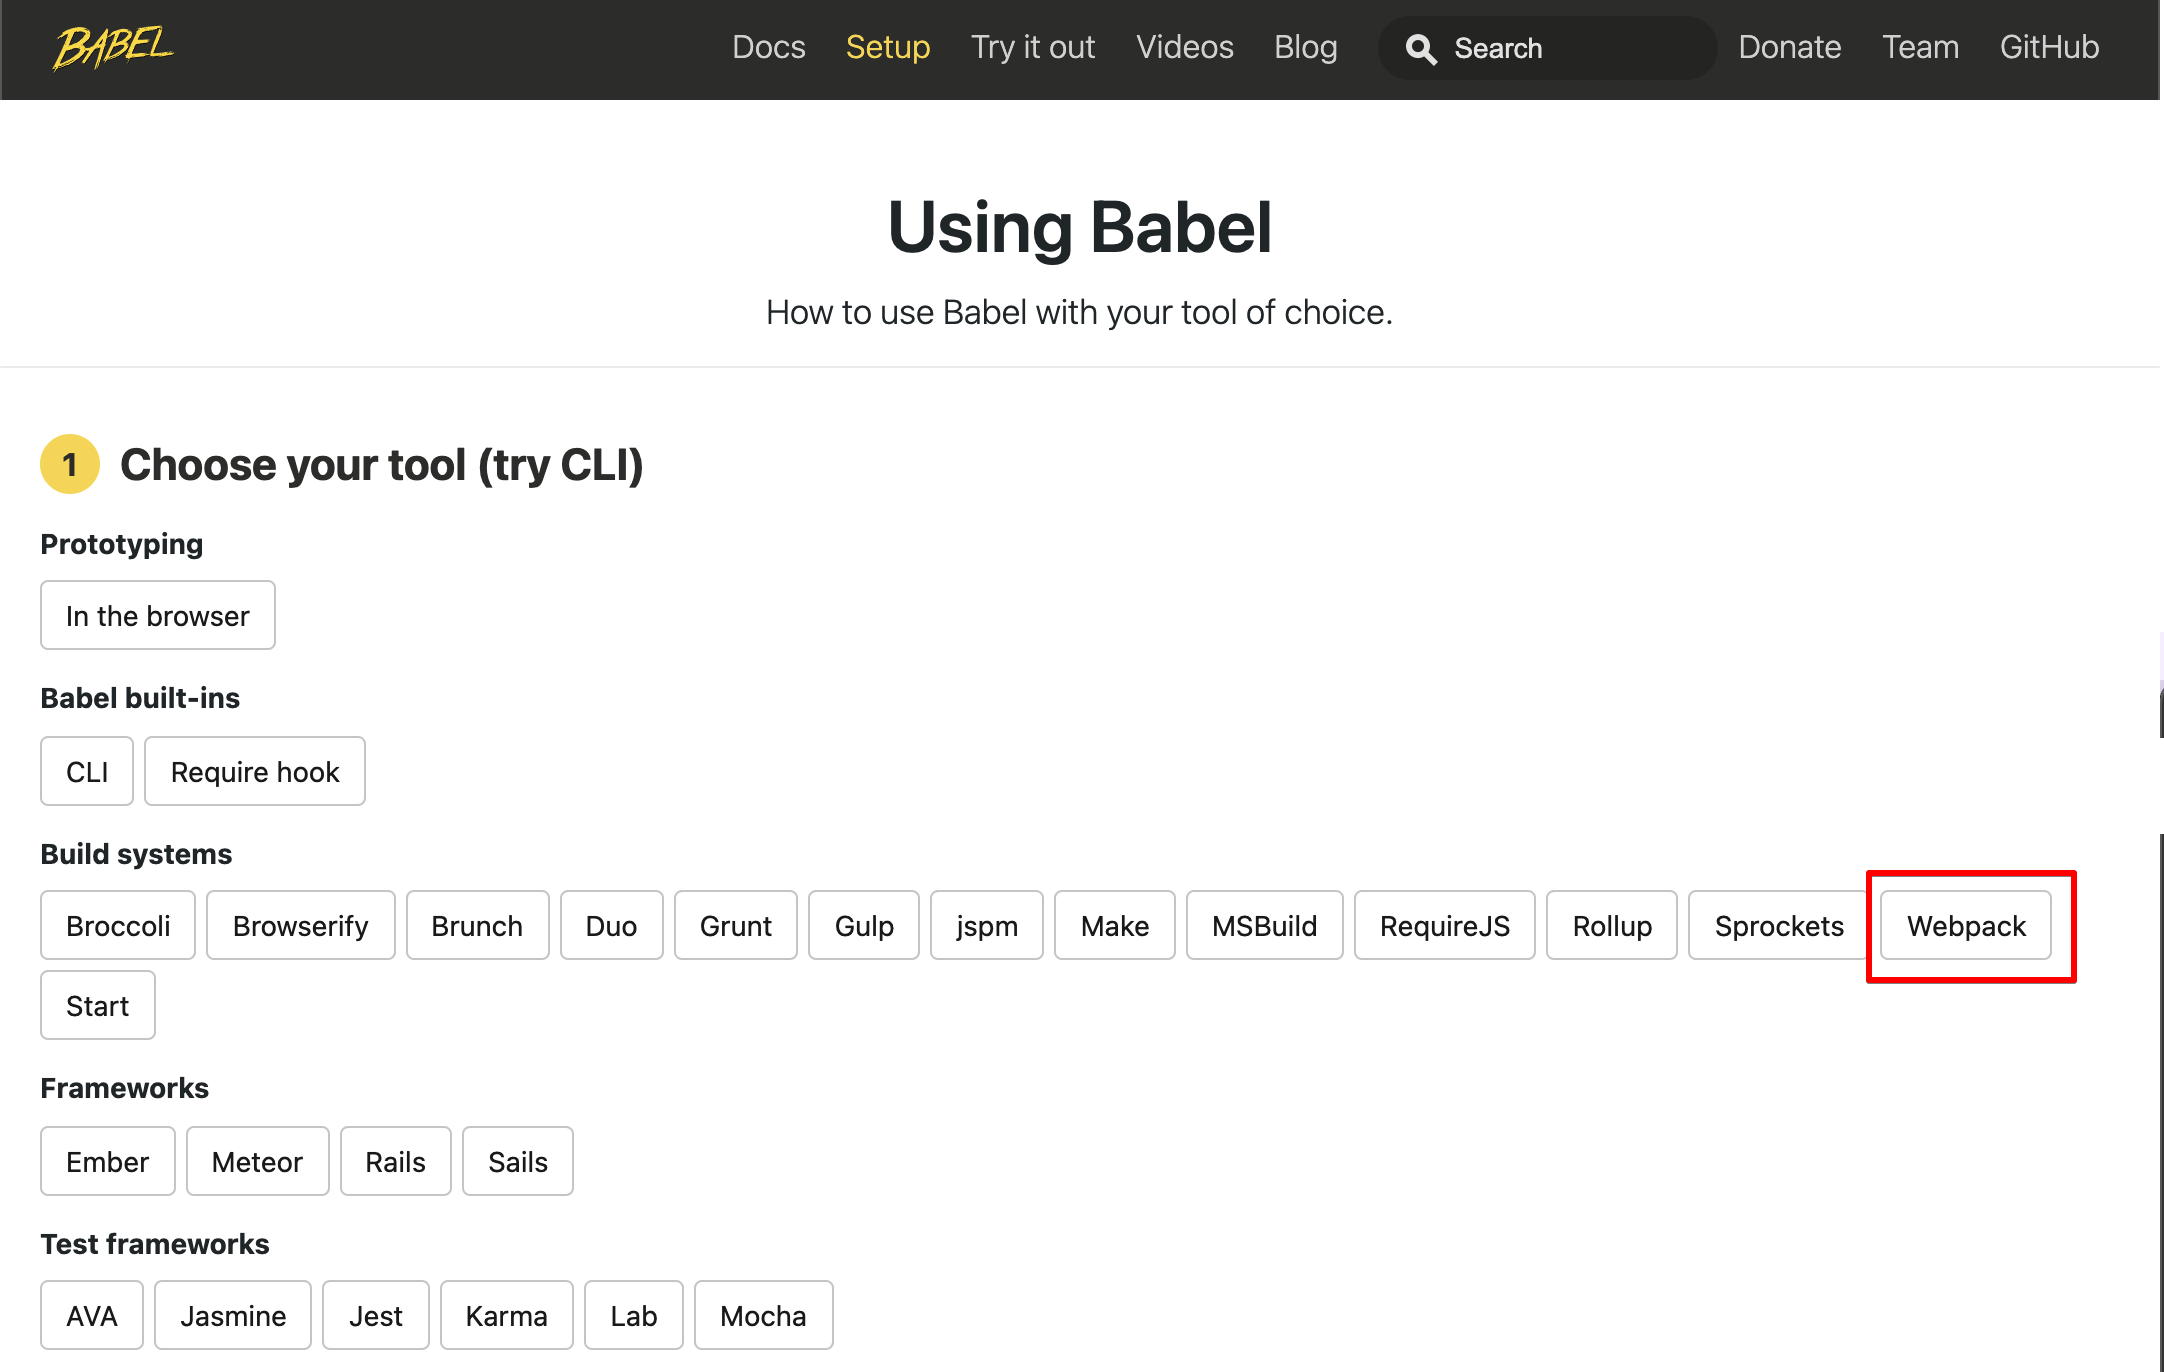
\includegraphics[width=1.0\maxwidth]{./images/02-create-react-app/babel02.png}%
\reviewimagecaption{使用するツールを選択}
\label{image:02-create-react-app:babel02}
\end{reviewimage}

このプロジェクトでは、「webpack」を使用しますので、「webpack」ボタンをクリックします。

\vspace*{\baselineskip}

手順2〜4が表示されましたので、順に実行していきます。

\begin{reviewimage}%%babel03
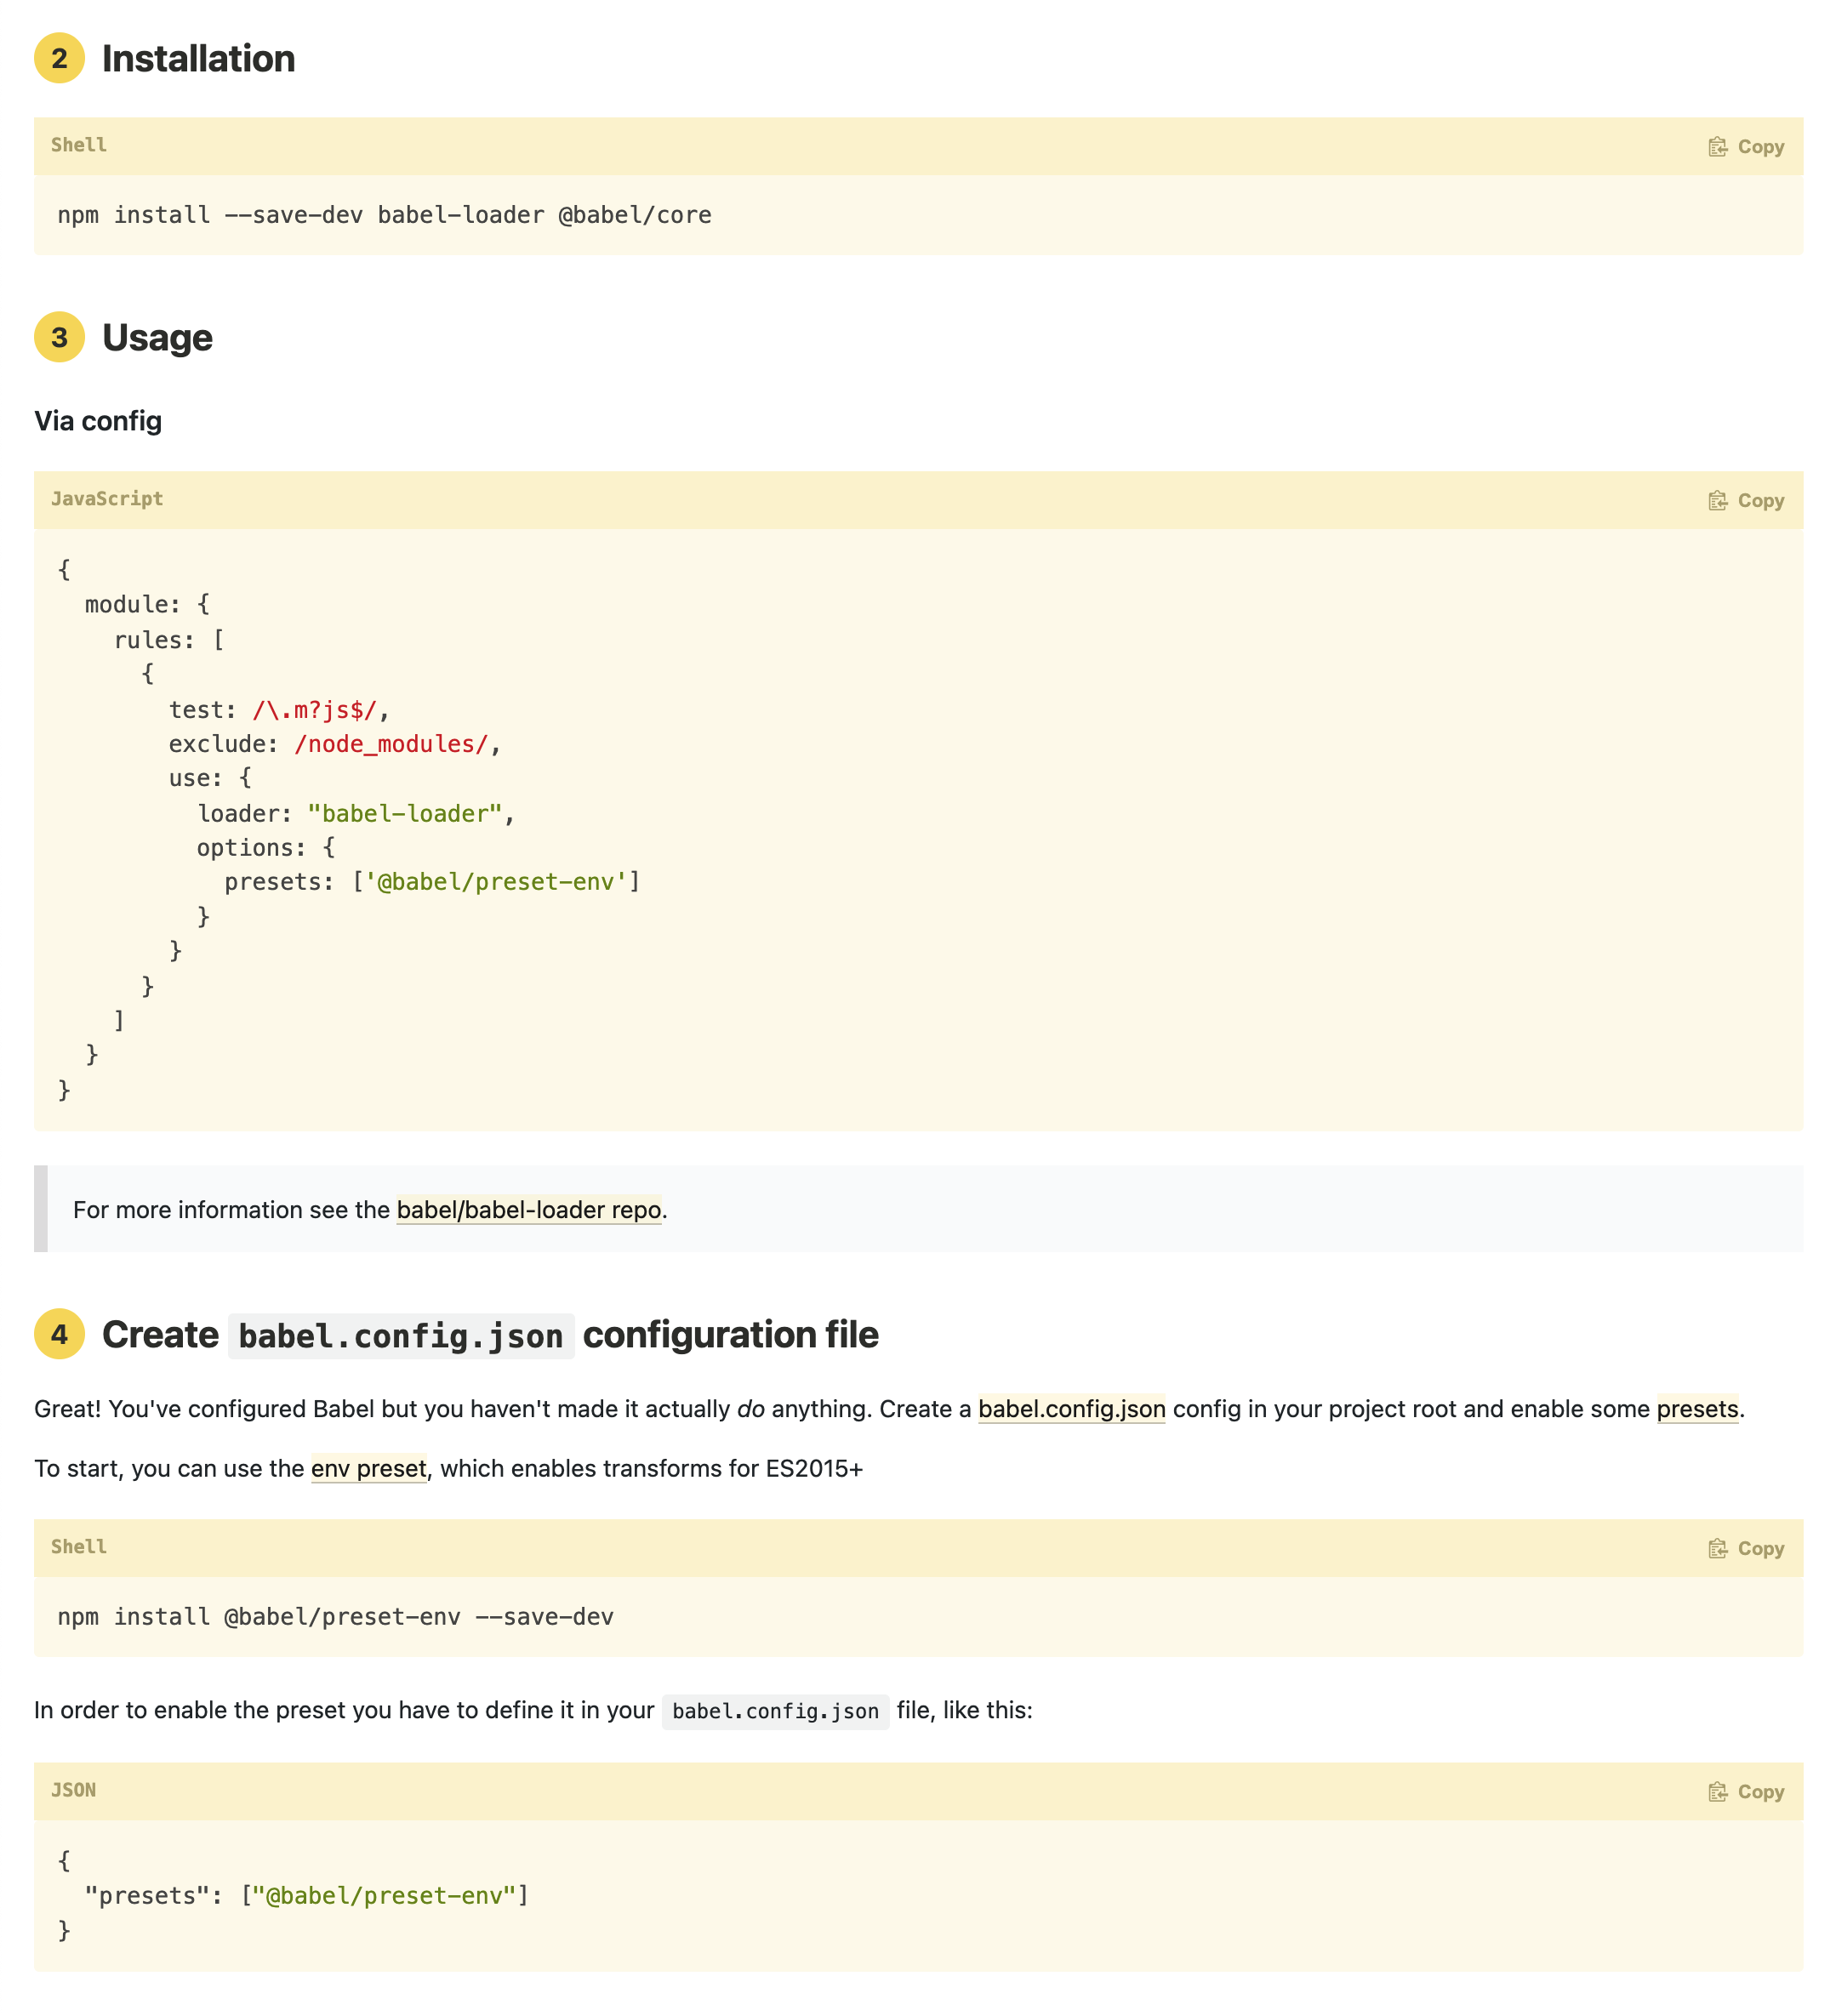
\includegraphics[width=1.0\maxwidth]{./images/02-create-react-app/babel03.png}%
\reviewimagecaption{パッケージのpa}
\label{image:02-create-react-app:babel03}
\end{reviewimage}

\clearpage


最初に指示されているパッケージをインストールします。今までnpmでインストール時に「{-}D」としていたのは、
「{-}{-}save{-}dev」の略です。
右端にあるコピーアイコンをクリックしてターミナルに貼り付けても良いです。

\def\startercodeblockfontsize{}
\begin{starterterminal}[]{Babel.jsパッケージインストール}\seqsplit{ \textgreater{} npm install {-}{-}save{-}dev babel{-}loader @babel/core}\end{starterterminal}

次に、手順3のコードを「webpack.common.js」へコピーします。コピー後の「webpack.common.js」です。

\def\startercodeblockfontsize{}
\begin{starterprogram}[]{webpack.common.js,Babelローダの導入}\seqsplit{  const path = require('path');
  const HtmlWebpackPlugin = require('html{-}webpack{-}plugin');

  module.exports = \{
    entry: './src/index.js',
    output: \{
      path: path.resolve(\textunderscore{}\textunderscore{}dirname, 'public'),
      assetModuleFilename: 'images/[name][ext][query]',
      clean: true,
    \},
    plugins: [
      new HtmlWebpackPlugin(\{
        template: 'index.html',
      \}),
    ],
    module: \{
      rules: [
        \{
          test: /\reviewbackslash{}.(ts\textbar{}tsx)\textdollar{}/i,
          loader: 'ts{-}loader',
          exclude: ['/node\textunderscore{}modules/'],
        \},
        \{
          test: /\reviewbackslash{}.m?js\textdollar{}/,
          exclude: /node\textunderscore{}modules/,
          use: \{
            loader: 'babel{-}loader',
            options: \{
              presets: ['@babel/preset{-}env'],
            \},
          \},
        \},
        \{
          test: /\reviewbackslash{}.(eot\textbar{}svg\textbar{}ttf\textbar{}woff\textbar{}woff2\textbar{}png\textbar{}jpg\textbar{}gif)\textdollar{}/i,
          type: 'asset',
        \},
      ],
    \},
    resolve: \{
      extensions: ['.tsx', '.ts', '.js'],
    \},
  \};
}\end{starterprogram}

次に、手順4に進みます。最初に「@babel/preset{-}env」パッケージをインストールします。

\def\startercodeblockfontsize{}
\begin{starterterminal}[]{@babel/preset{-}envのインストール}\seqsplit{ \textgreater{} npm install {-}{-}save{-}dev @babel/preset{-}env}\end{starterterminal}

インストールが完了しましたら、プロジェクトフォルダ直下に「babel.config.json」ファイルを作成し、手順4の内容を貼り付けます。

\def\startercodeblockfontsize{}
\begin{starterprogram}[]{babel.config.json}\seqsplit{  \{
    "presets": ["@babel/preset{-}env"]
  \}}\end{starterprogram}

以上で、Babel.jsの導入は完了です。

\subsubsection*{動作を確認してみる。}
\keeplastskip{
  \label{sec:2-2-6-1}
  \par\nobreak
}

「src/index.js」に少しコードを追加します。
ES6で新しく使えるようになったテンプレートリテラルを使用したコードです。

\def\startercodeblockfontsize{}
\begin{starterprogram}[]{src/index.js}\seqsplit{  import \textunderscore{} from 'lodash';
  import './style.css';
  import './style.scss';

  import Yaruo from './assets/images/yaruo.png';

  function component() \{
    const element = document.createElement('div');

    // Lodash, now imported by this script
    const myName = 'やる夫';
    const words = 'こまけぇこたぁいいんだよ〜';
    const message = `\textless{}br /\textgreater{}\textdollar{}\{myName\}の口グセなのか?\textless{}br /\textgreater{}\textdollar{}\{words\}`;
    element.innerHTML = \textunderscore{}.join(['webpack', '動いてるお〜'], ' ') + message;

    return element;
  \}

  document.body.appendChild(component());

  const image = new Image();
  image.src = Yaruo;

  document.body.appendChild(image);
}\end{starterprogram}

\clearpage


Babel.js導入前の実行結果です。

\begin{reviewimage}%%babel06
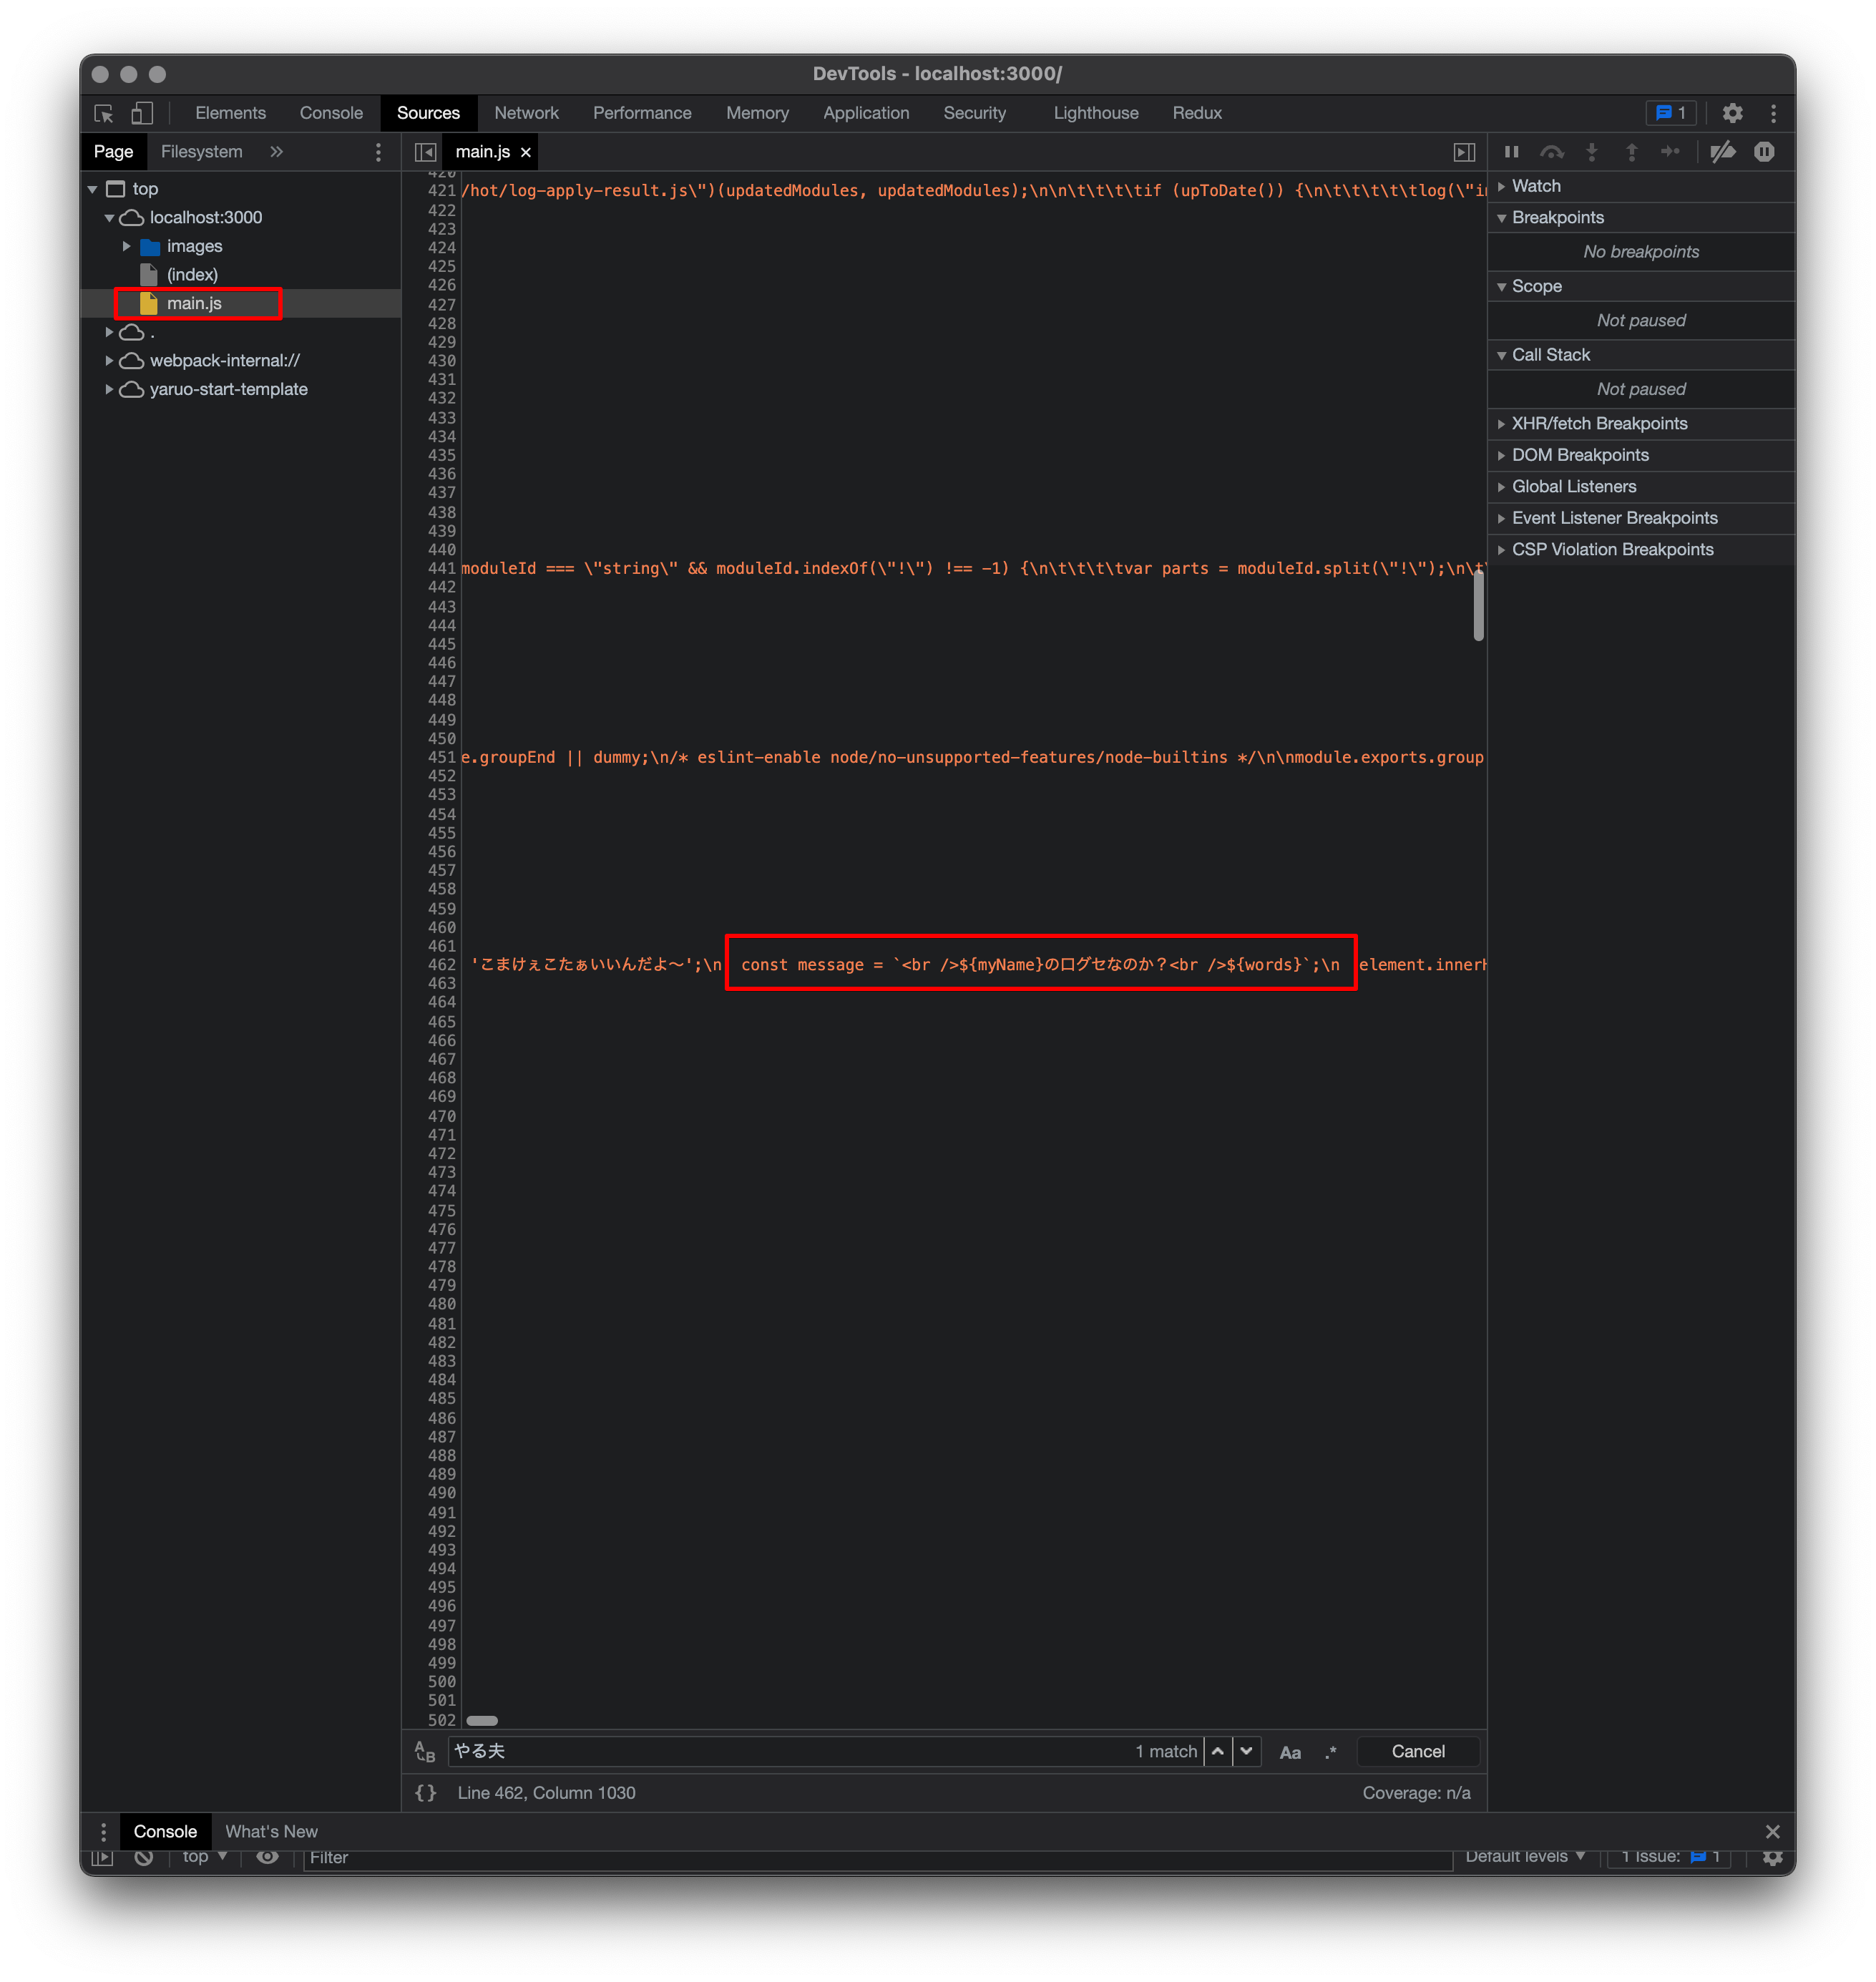
\includegraphics[width=0.9\maxwidth]{./images/02-create-react-app/babel06.png}%
\reviewimagecaption{Babel.js導入前ですので、そのまま}
\label{image:02-create-react-app:babel06}
\end{reviewimage}

\clearpage


Babel.js導入後の実行結果です。

\begin{reviewimage}%%babel07
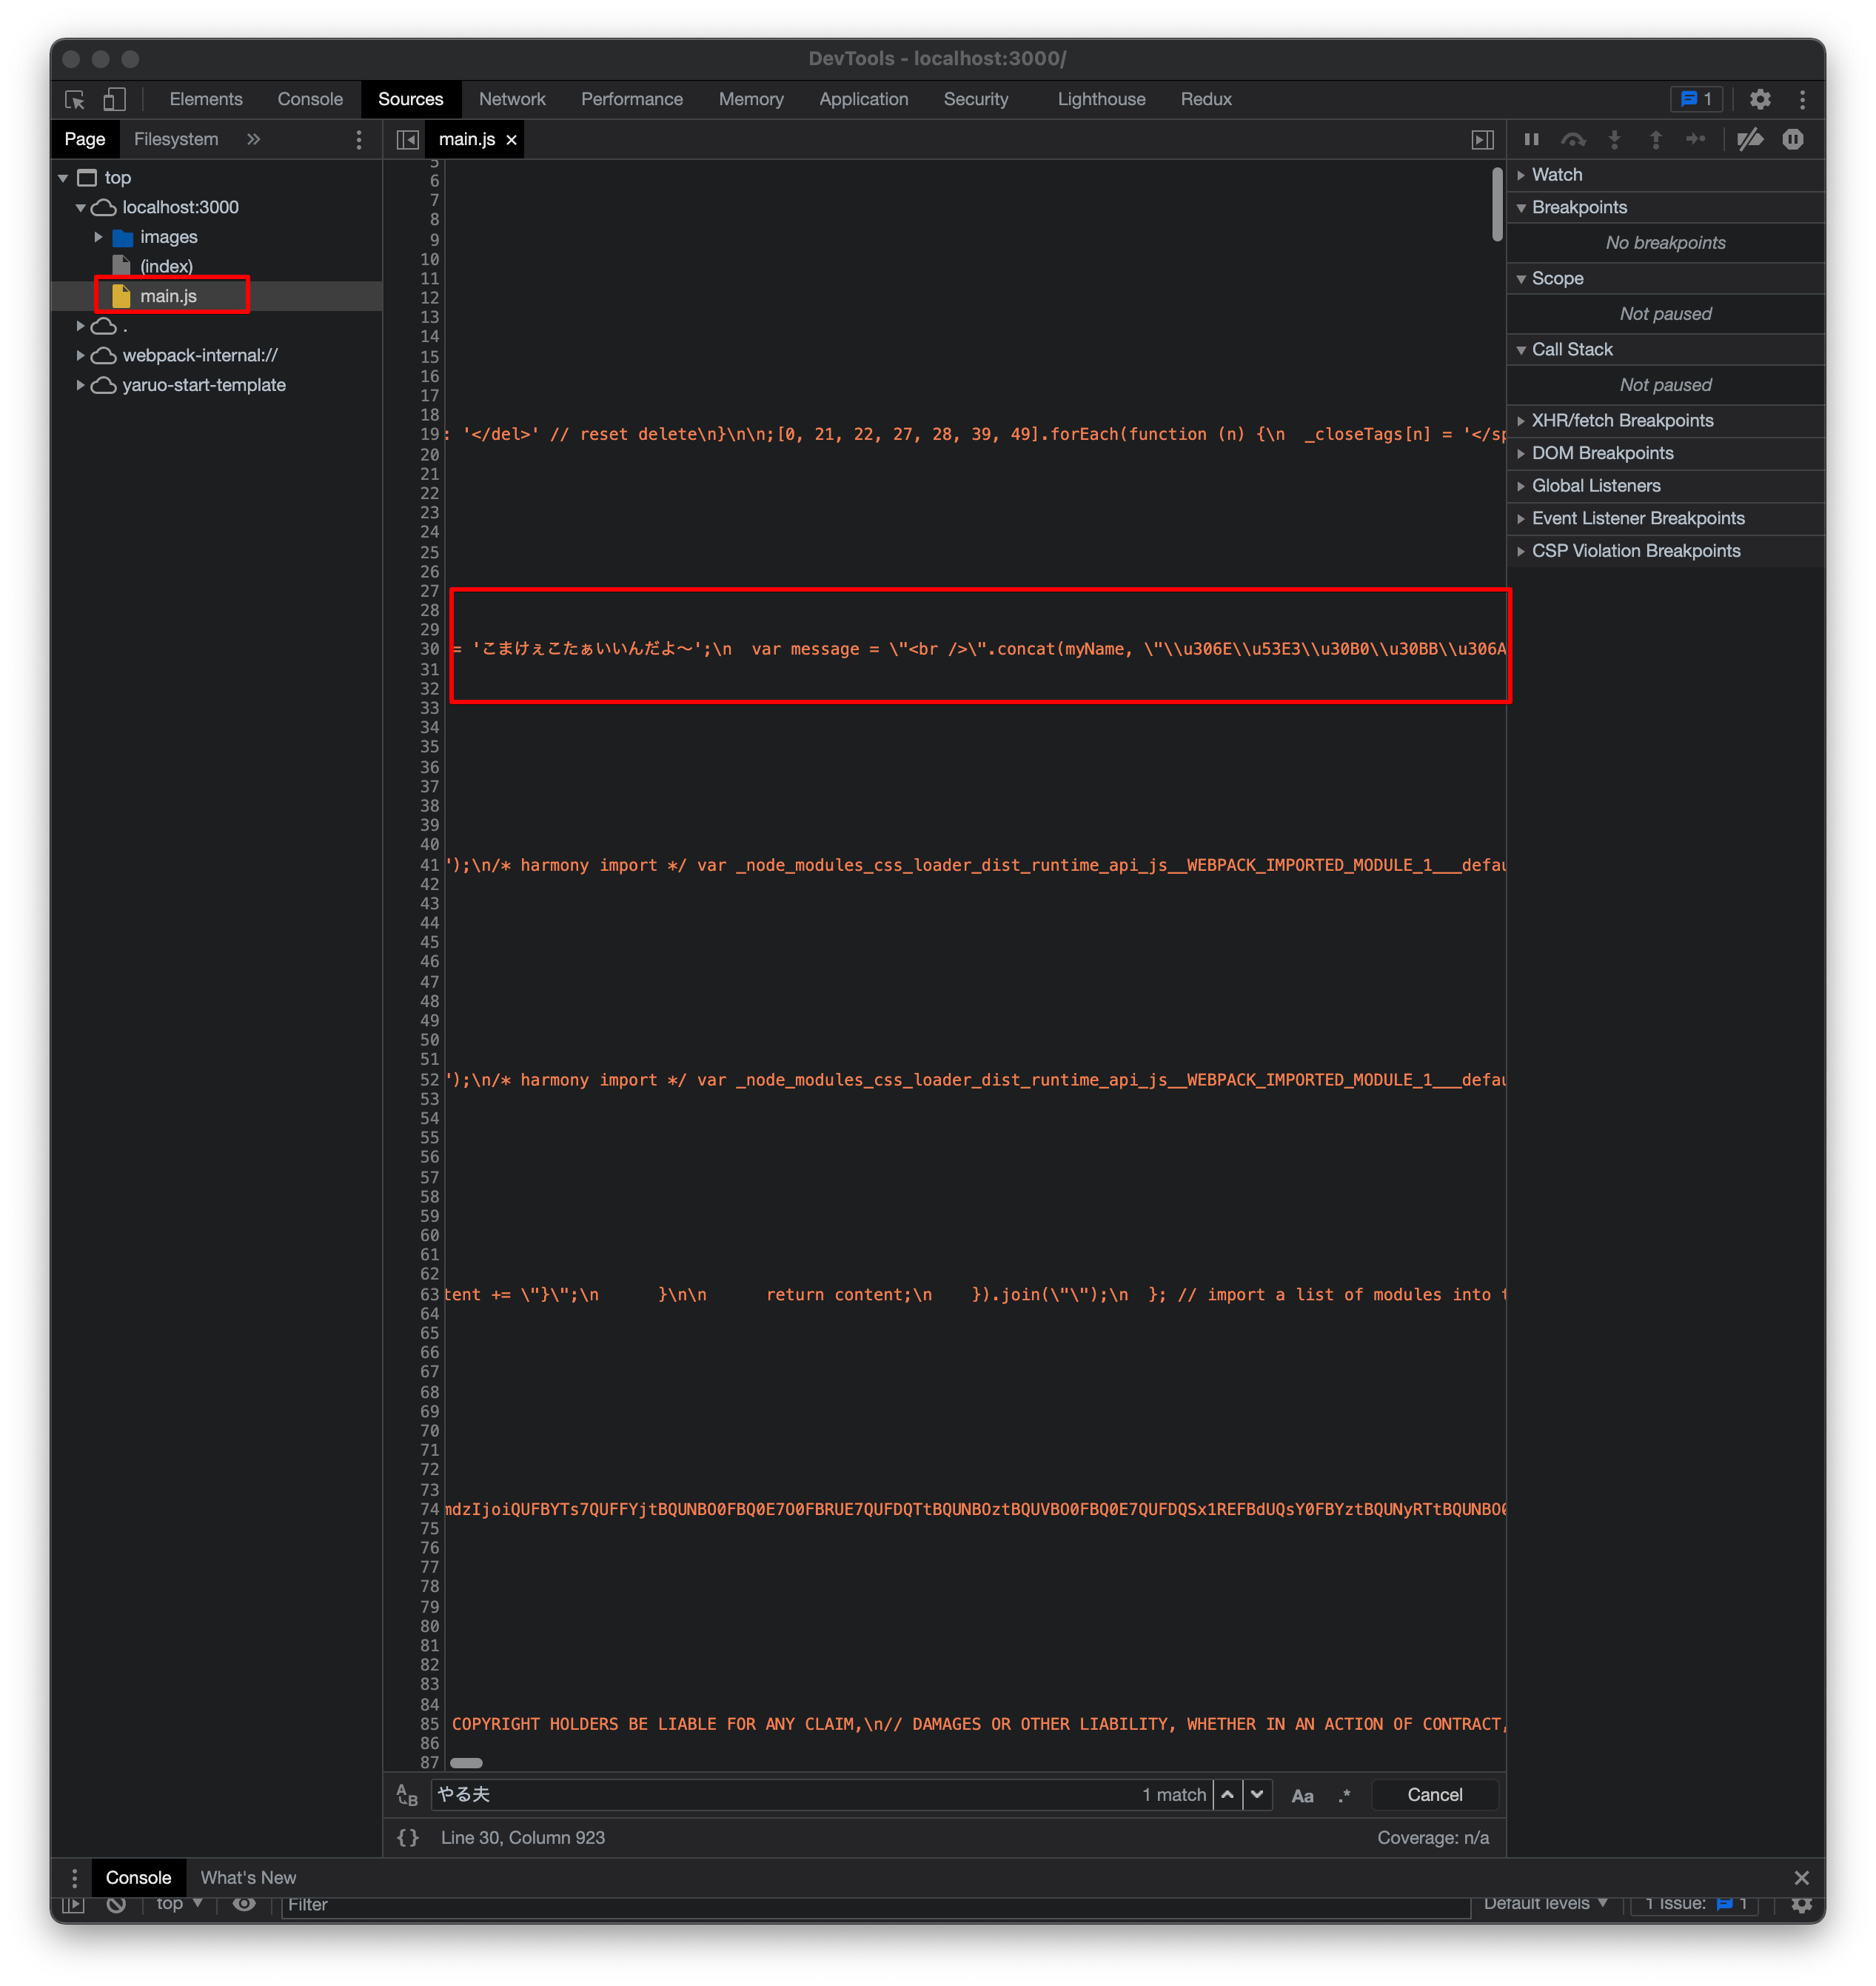
\includegraphics[width=0.9\maxwidth]{./images/02-create-react-app/babel07.png}%
\reviewimagecaption{concatに変換されています。}
\label{image:02-create-react-app:babel07}
\end{reviewimage}
\begin{starternote}[]{}

ここまでの内容は、GitHub上で、以下のコマンドでクローンできます。

\def\startercodeblockfontsize{}
\begin{starterterminal}[]{GitHub}\seqsplit{\textgreater{} git clone {-}b 05\textunderscore{}babel{-}install https://github.com/yaruo{-}react{-}redux/yaruo{-}start{-}template.git}\end{starterterminal}
\end{starternote}

\subsection{Reactのインストール}
\keeplastskip{
  \label{sec:2-2-7}
  \label{sec04-react}
  \par\nobreak
}
\begin{starterwarning}{index.tsを削除してね。}

ここで気が付いたのですが、「src/index.ts」は、現時点で不要なので削除してください。

\end{starterwarning}

そろそろ完成に近付いてきました。Reactをインストールします。

\vspace*{\baselineskip}

Reactは、拡張子「.jsx」を使ったHTMLにJavaScriptを埋め込むコンポーネントがメインです。
通常のJavaScriptとは記法が違うため「Babel.js」に理解してもらえるように「@babel/preset{-}react」を
インストールします。

\begin{reviewimage}%%babel08
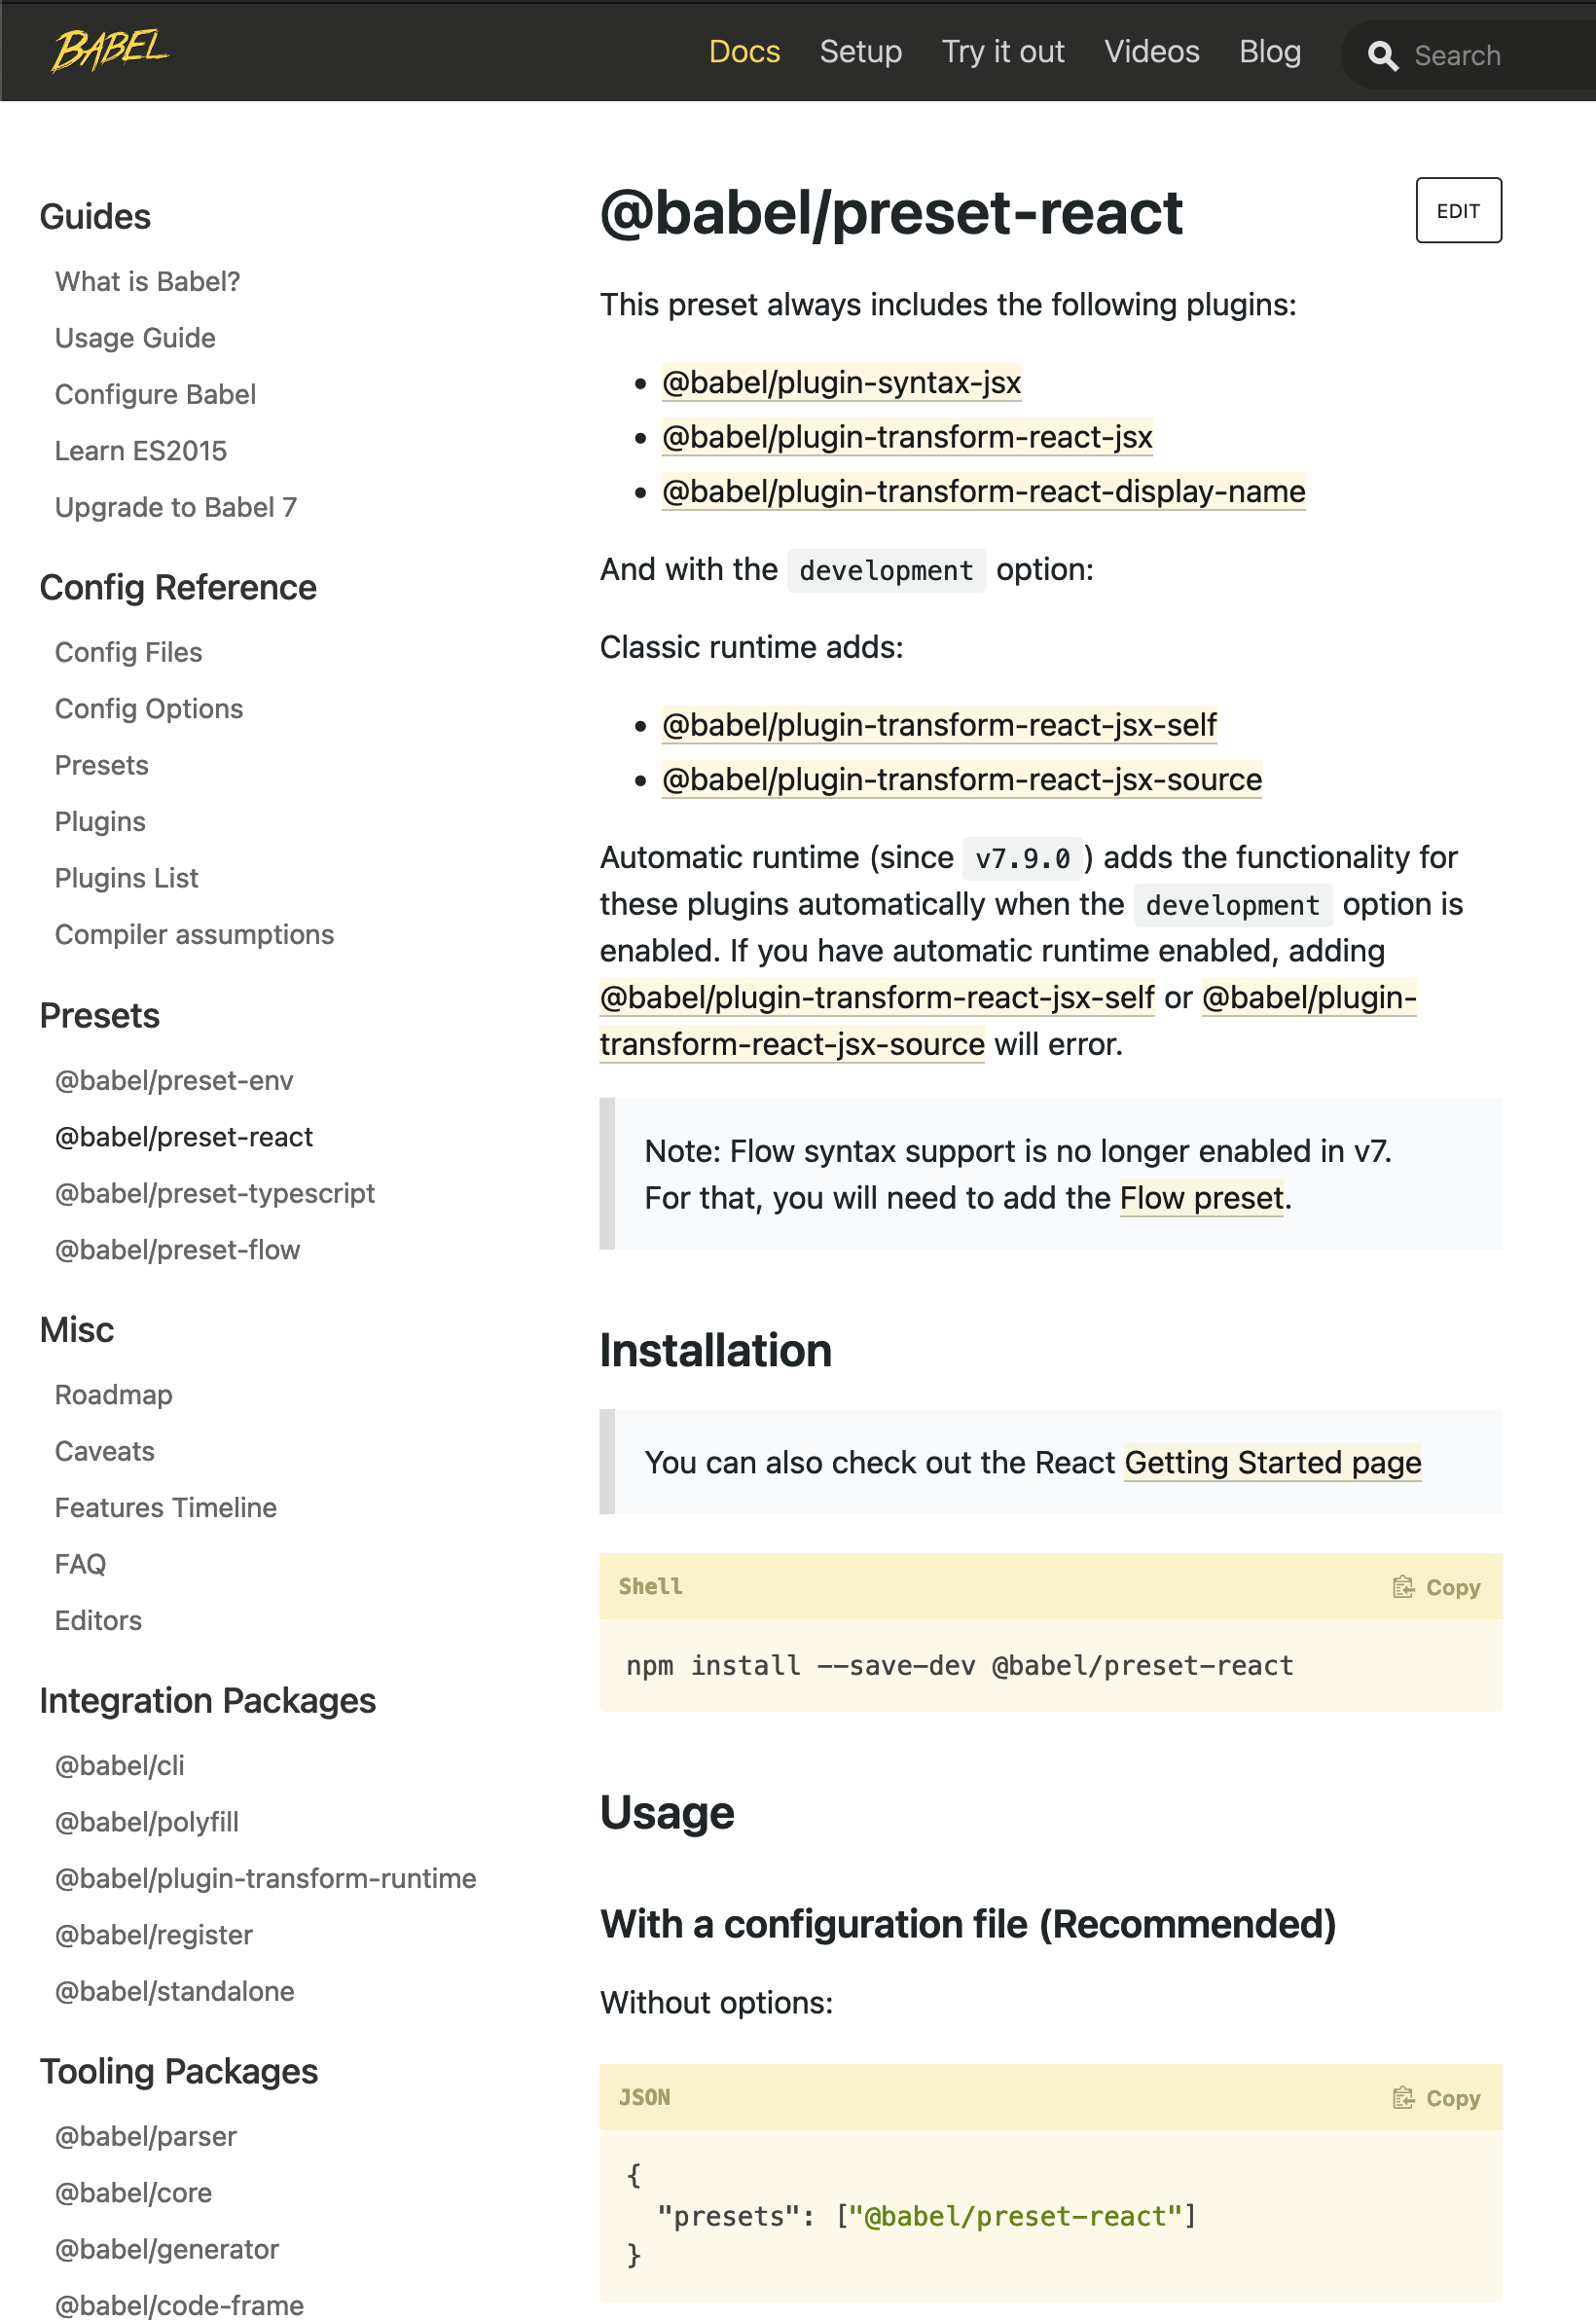
\includegraphics[width=0.9\maxwidth]{./images/02-create-react-app/babel08.png}%
\reviewimagecaption{@babel/preset{-}react}
\label{image:02-create-react-app:babel08}
\end{reviewimage}

\clearpage


ターミナルに以下のコマンドでインストールします。

\def\startercodeblockfontsize{}
\begin{starterterminal}[]{@babel/preset{-}reactのインストール}\seqsplit{ \textgreater{} npm install {-}D @babel/preset{-}react}\end{starterterminal}

インストールが完了しましたら、「babel.config.json」へプリセットを追加します。

\def\startercodeblockfontsize{}
\begin{starterprogram}[]{babel.config.json}\seqsplit{  \{
    "presets": [["@babel/preset{-}env"], ["@babel/preset{-}react"]]
  \}}\end{starterprogram}
\vspace*{\baselineskip}

Reactを使うためにインストールするパッケージは、

\begin{starteritemize}
\item react(react本体)
\item react{-}dom(DOMへのエントリポイント、Reactの描画を提供)
\end{starteritemize}

の2つです。

\def\startercodeblockfontsize{}
\begin{starterterminal}[]{Reactのインストール}\seqsplit{ \textgreater{} npm install react react{-}dom}\end{starterterminal}

以上で、Reactのインストールは完了しましたので動作確認を行います。

\vspace*{\baselineskip}

手順は、

\begin{starterenumerate}
\item src/index.htmlに描画する場所を指定する。
\item src/index.jsで上記「index.html」へReactDOMで描画する。
\item Appコンポーネントをsrc/components/App.jsxファイルへ作成する。
\item 「webpack.common.js」へReactコンポーネント「jsx」を扱うよう変更する。
\end{starterenumerate}

となります。

「src/index.html」は、Reactの描画する部分を指定します。

\def\startercodeblockfontsize{}
\begin{starterprogram}[]{src/index.html}\seqsplit{  \textless{}!DOCTYPE html\textgreater{}
  \textless{}html\textgreater{}
    \textless{}head\textgreater{}
      \textless{}meta charset="utf{-}8" /\textgreater{}
      \textless{}title\textgreater{}React Appだお〜\textless{}/title\textgreater{}
    \textless{}/head\textgreater{}
    \textless{}body\textgreater{}
      \textless{}div id="root"\textgreater{}\textless{}/div\textgreater{}
    \textless{}/body\textgreater{}
  \textless{}/html\textgreater{}
}\end{starterprogram}

「src/index.js」にてReactDOMを使用して「public/index.html」へ描画する。

\def\startercodeblockfontsize{}
\begin{starterprogram}[]{src/index.js}\seqsplit{  import React from 'react';
  import ReactDOM from 'react{-}dom';
  import App from './App';

  ReactDOM.render(
    \textless{}div\textgreater{}
      \textless{}App /\textgreater{}
    \textless{}/div\textgreater{},
    document.getElementById('root')
  );}\end{starterprogram}

「src/components/App.jsx」にAppコンポーネントを作成します。Reactコンポーネントは、
HTML内にJavaScriptを埋め込む記法となります。

\def\startercodeblockfontsize{}
\begin{starterprogram}[]{src/components/App.jsx}\seqsplit{  import React from 'react';
  import \textunderscore{} from 'lodash';
  import Yaruo from '../assets/images/yaruo.png';

  const App = () =\textgreater{} \{
    const myName = 'やる夫';
    const words = 'こまけぇこたぁいいんだよ〜';
    return (
      \textless{}div\textgreater{}
        \{\textunderscore{}.join(['webpack', '動いてるお〜'], ' ')\}
        \textless{}br /\textgreater{}
        \{myName\}口グセなのか?
        \textless{}br /\textgreater{}
        \{words\}
        \textless{}div\textgreater{}
          \textless{}img src=\{Yaruo\} /\textgreater{}
        \textless{}/div\textgreater{}
      \textless{}/div\textgreater{}
    );
  \};

  export default App;}\end{starterprogram}

「webpack.common.js」を以下のように変更します。

\begin{starteritemize}
\item Reactコンポーネントの拡張子「.jsx」を扱うように変更する。
\item テンプレートを「src/index.html」に変更する。
\end{starteritemize}

\def\startercodeblockfontsize{}
\begin{starterprogram}[]{webpack.common.js}\seqsplit{  const path = require('path');
  const HtmlWebpackPlugin = require('html{-}webpack{-}plugin');

  module.exports = \{
    entry: './src/index.js',
    output: \{
      path: path.resolve(\textunderscore{}\textunderscore{}dirname, 'public'),
      assetModuleFilename: 'images/[name][ext][query]',
      clean: true,
    \},
    plugins: [
      new HtmlWebpackPlugin(\{
        template: 'src/index.html',
      \}),
    ],
    module: \{
      rules: [
        \{
          test: /\reviewbackslash{}.(ts\textbar{}tsx)\textdollar{}/i,
          loader: 'ts{-}loader',
          exclude: ['/node\textunderscore{}modules/'],
        \},
        \{
          test: /\reviewbackslash{}.(js\textbar{}jsx)/i,
          exclude: /node\textunderscore{}modules/,
          use: \{
            loader: 'babel{-}loader',
            options: \{
              presets: ['@babel/preset{-}env'],
            \},
          \},
        \},
        \{
          test: /\reviewbackslash{}.(eot\textbar{}svg\textbar{}ttf\textbar{}woff\textbar{}woff2\textbar{}png\textbar{}jpg\textbar{}gif)\textdollar{}/i,
          type: 'asset',
        \},
      ],
    \},
    resolve: \{
      extensions: ['.tsx', '.ts', '.js', '.jsx'],
    \},
  \};
}\end{starterprogram}

動作確認を行います。

\def\startercodeblockfontsize{}
\begin{starterterminal}[]{reactの動作確認}\seqsplit{ \textgreater{} npm run start}\end{starterterminal}
\begin{reviewimage}%%babel09
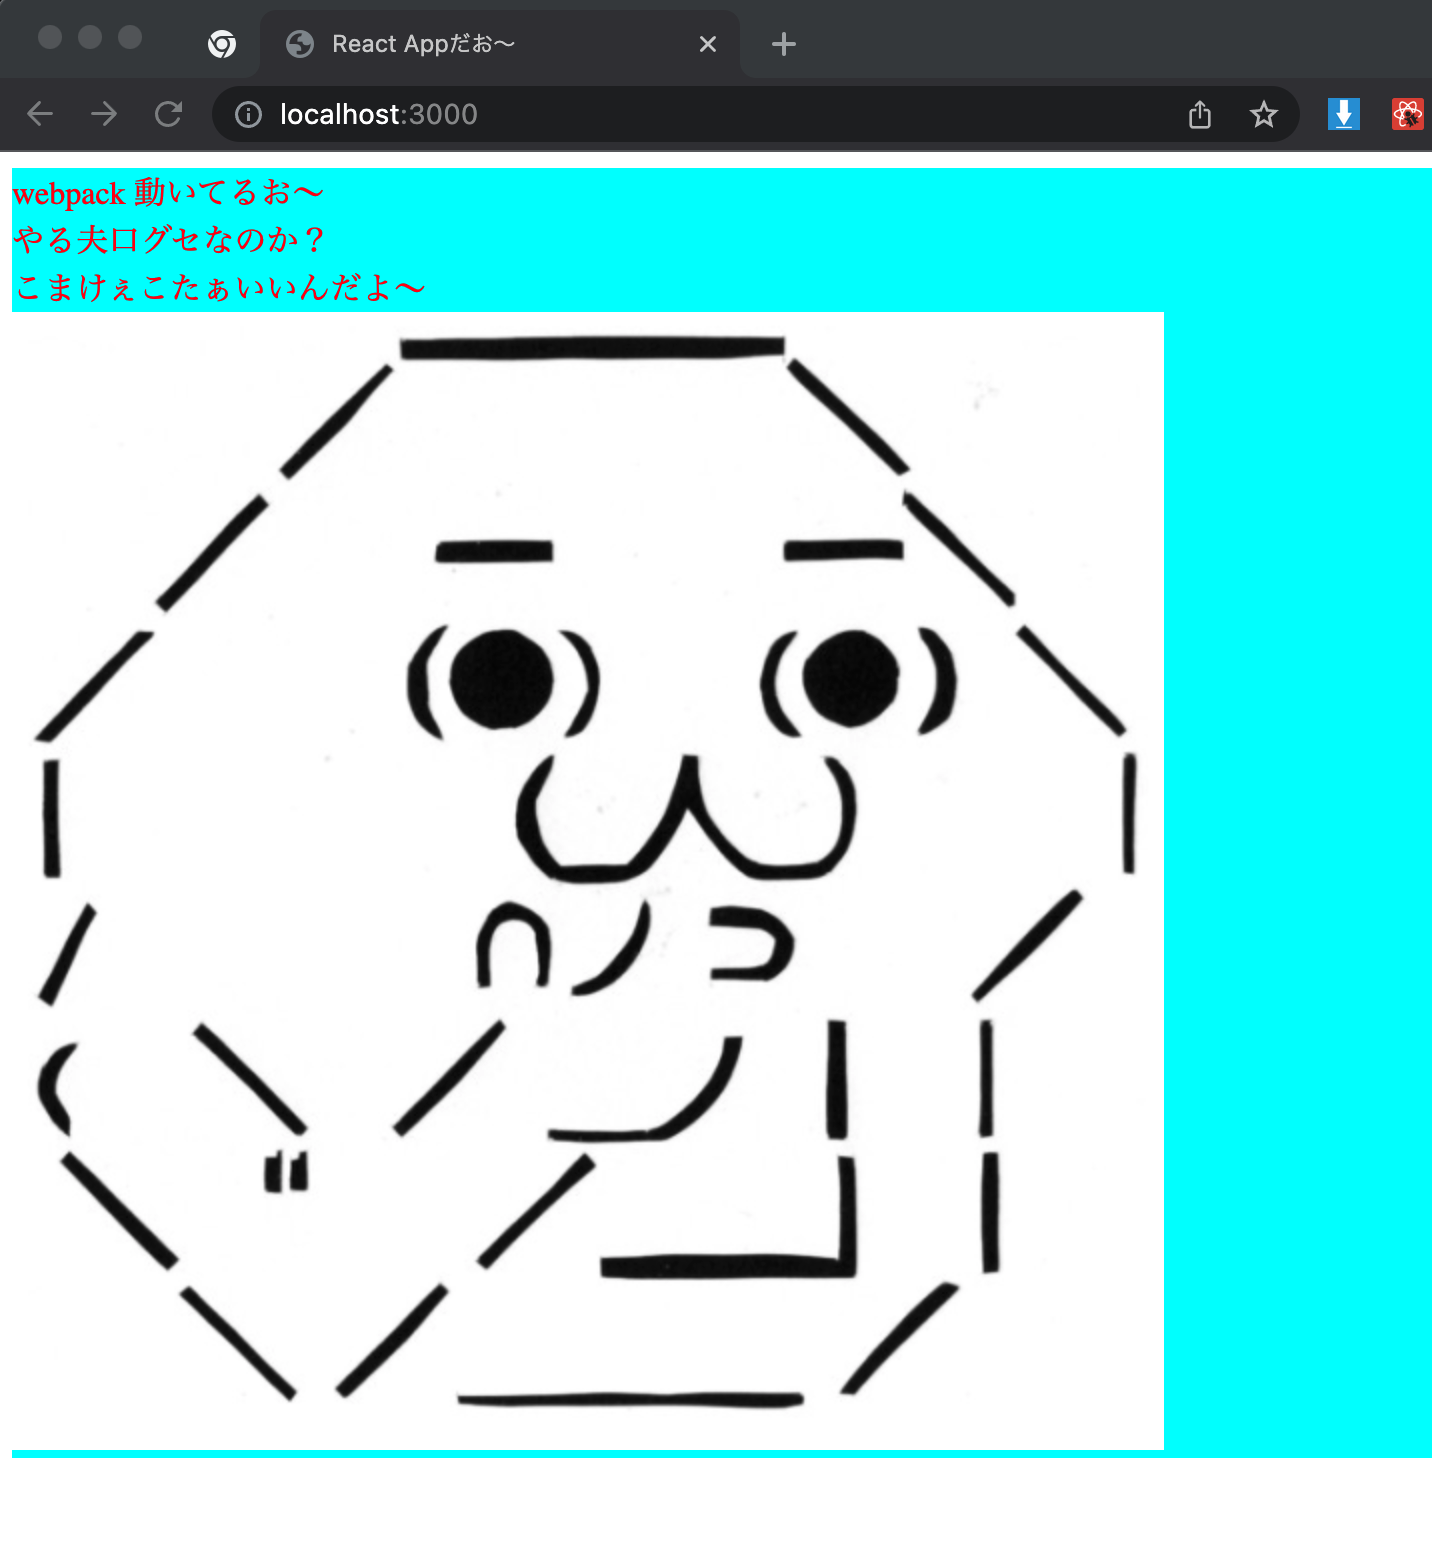
\includegraphics[width=1.0\maxwidth]{./images/02-create-react-app/babel09.png}%
\reviewimagecaption{reactの動作確認}
\label{image:02-create-react-app:babel09}
\end{reviewimage}
\begin{starternote}[]{}

ここまでの内容は、GitHub上で、以下のコマンドでクローンできます。

\def\startercodeblockfontsize{}
\begin{starterterminal}[]{GitHub}\seqsplit{\textgreater{} git clone {-}b 06\textunderscore{}react{-}install https://github.com/yaruo{-}react{-}redux/yaruo{-}start{-}template.git}\end{starterterminal}
\end{starternote}

\subsection{TypeScriptのインストール}
\keeplastskip{
  \label{sec:2-2-8}
  \label{sec04-typescript}
  \par\nobreak
}

ここまで作成したReactプロジェクトにTypeScriptを導入します。
本家Reactでは、TypeScriptの導入\footnote{\url{https://ja.reactjs.org/docs/static-type-checking.html\#typescript}}に関して
以下のような手順を示しています。

\begin{reviewimage}%%typescript01
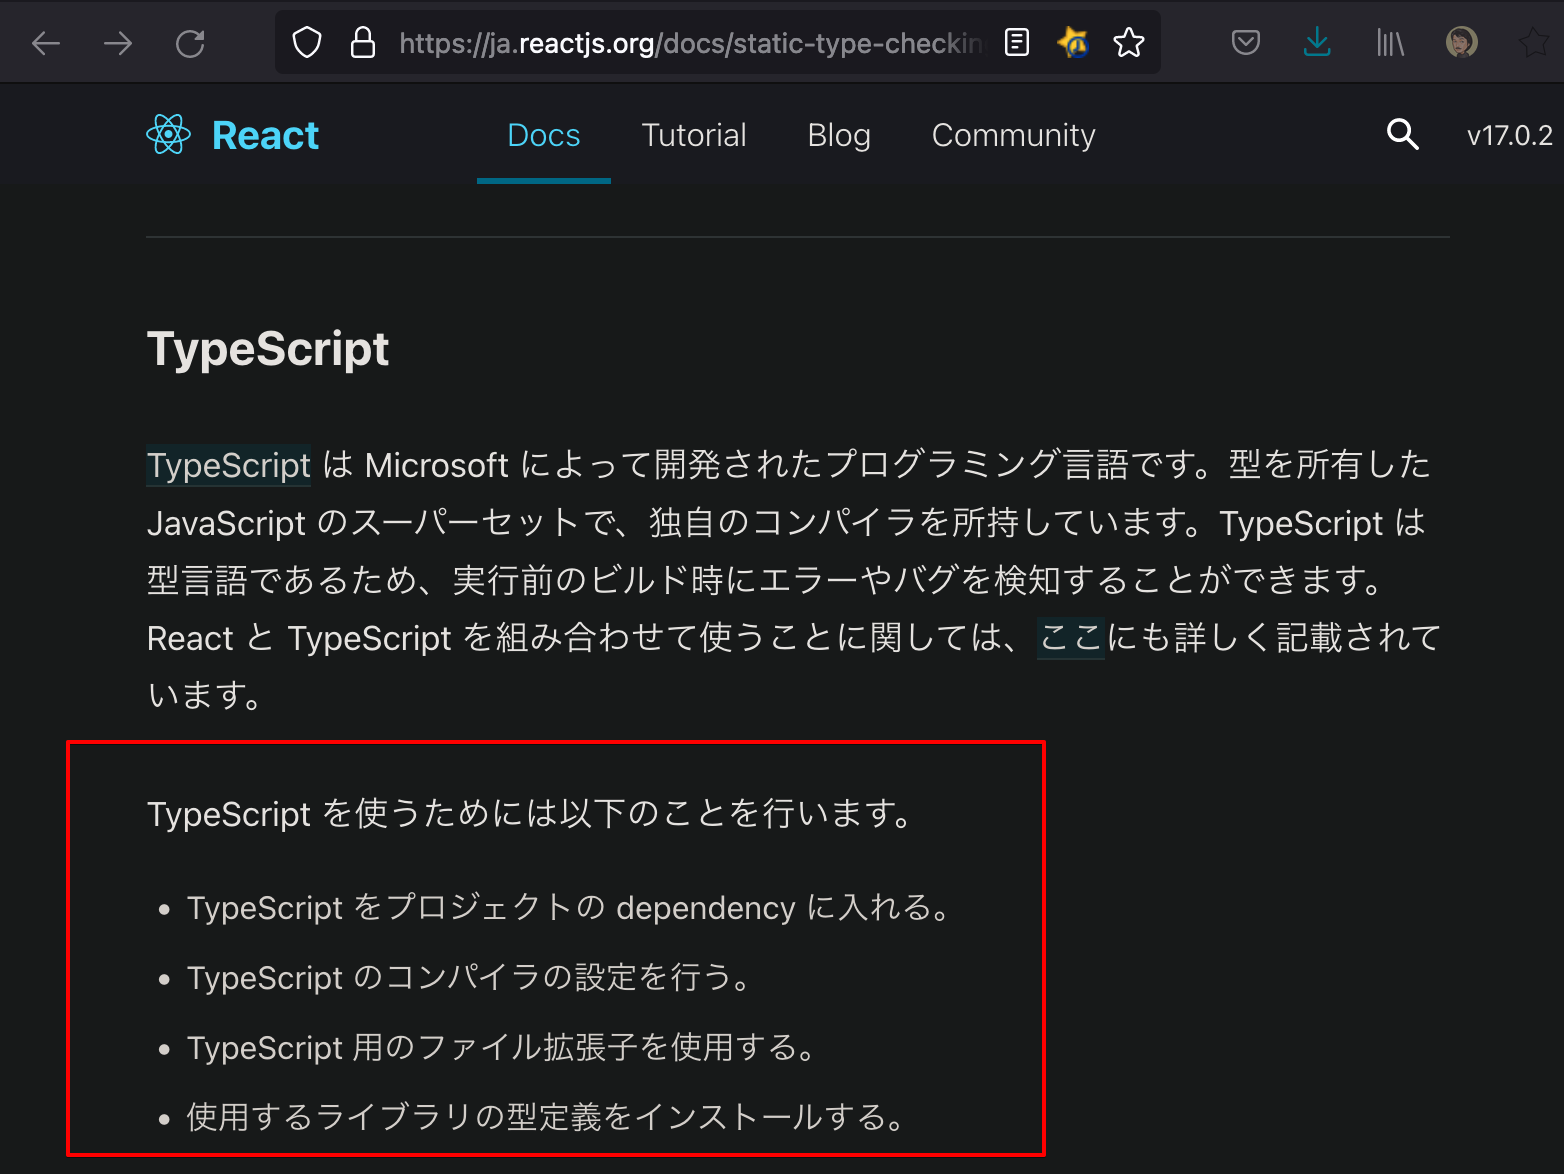
\includegraphics[width=0.8\maxwidth]{./images/02-create-react-app/typescript01.png}%
\reviewimagecaption{TypeScriptの導入}
\label{image:02-create-react-app:typescript01}
\end{reviewimage}

では手順に従って、TypeScriptを導入していきます。

\vspace*{\baselineskip}

最初は、TypeScriptパッケージのインストールです。

\def\startercodeblockfontsize{}
\begin{starterterminal}[]{TypeScriptパッケージのインストール}\seqsplit{ \textgreater{} npm install {-}D typescript}\end{starterterminal}

次に、TypeScriptのコンパイラ設定ファイル「tsconfig.json」を作成します。

\def\startercodeblockfontsize{}
\begin{starterterminal}[]{tsconfig.jsonの作成}\seqsplit{ \textgreater{} npx tsc {-}{-}init

Created a new tsconfig.json with:
                                                                                                                  TS
  target: es2016
  module: commonjs
  strict: true
  esModuleInterop: true
  skipLibCheck: true
  forceConsistentCasingInFileNames: true


You can learn more at https://aka.ms/tsconfig.json}\end{starterterminal}

コマンドを実行すると、「tsconfig.json」ファイルが作成されます。
コメントアウトされているものは、デフォルト値です。

\begin{reviewimage}%%typescript04
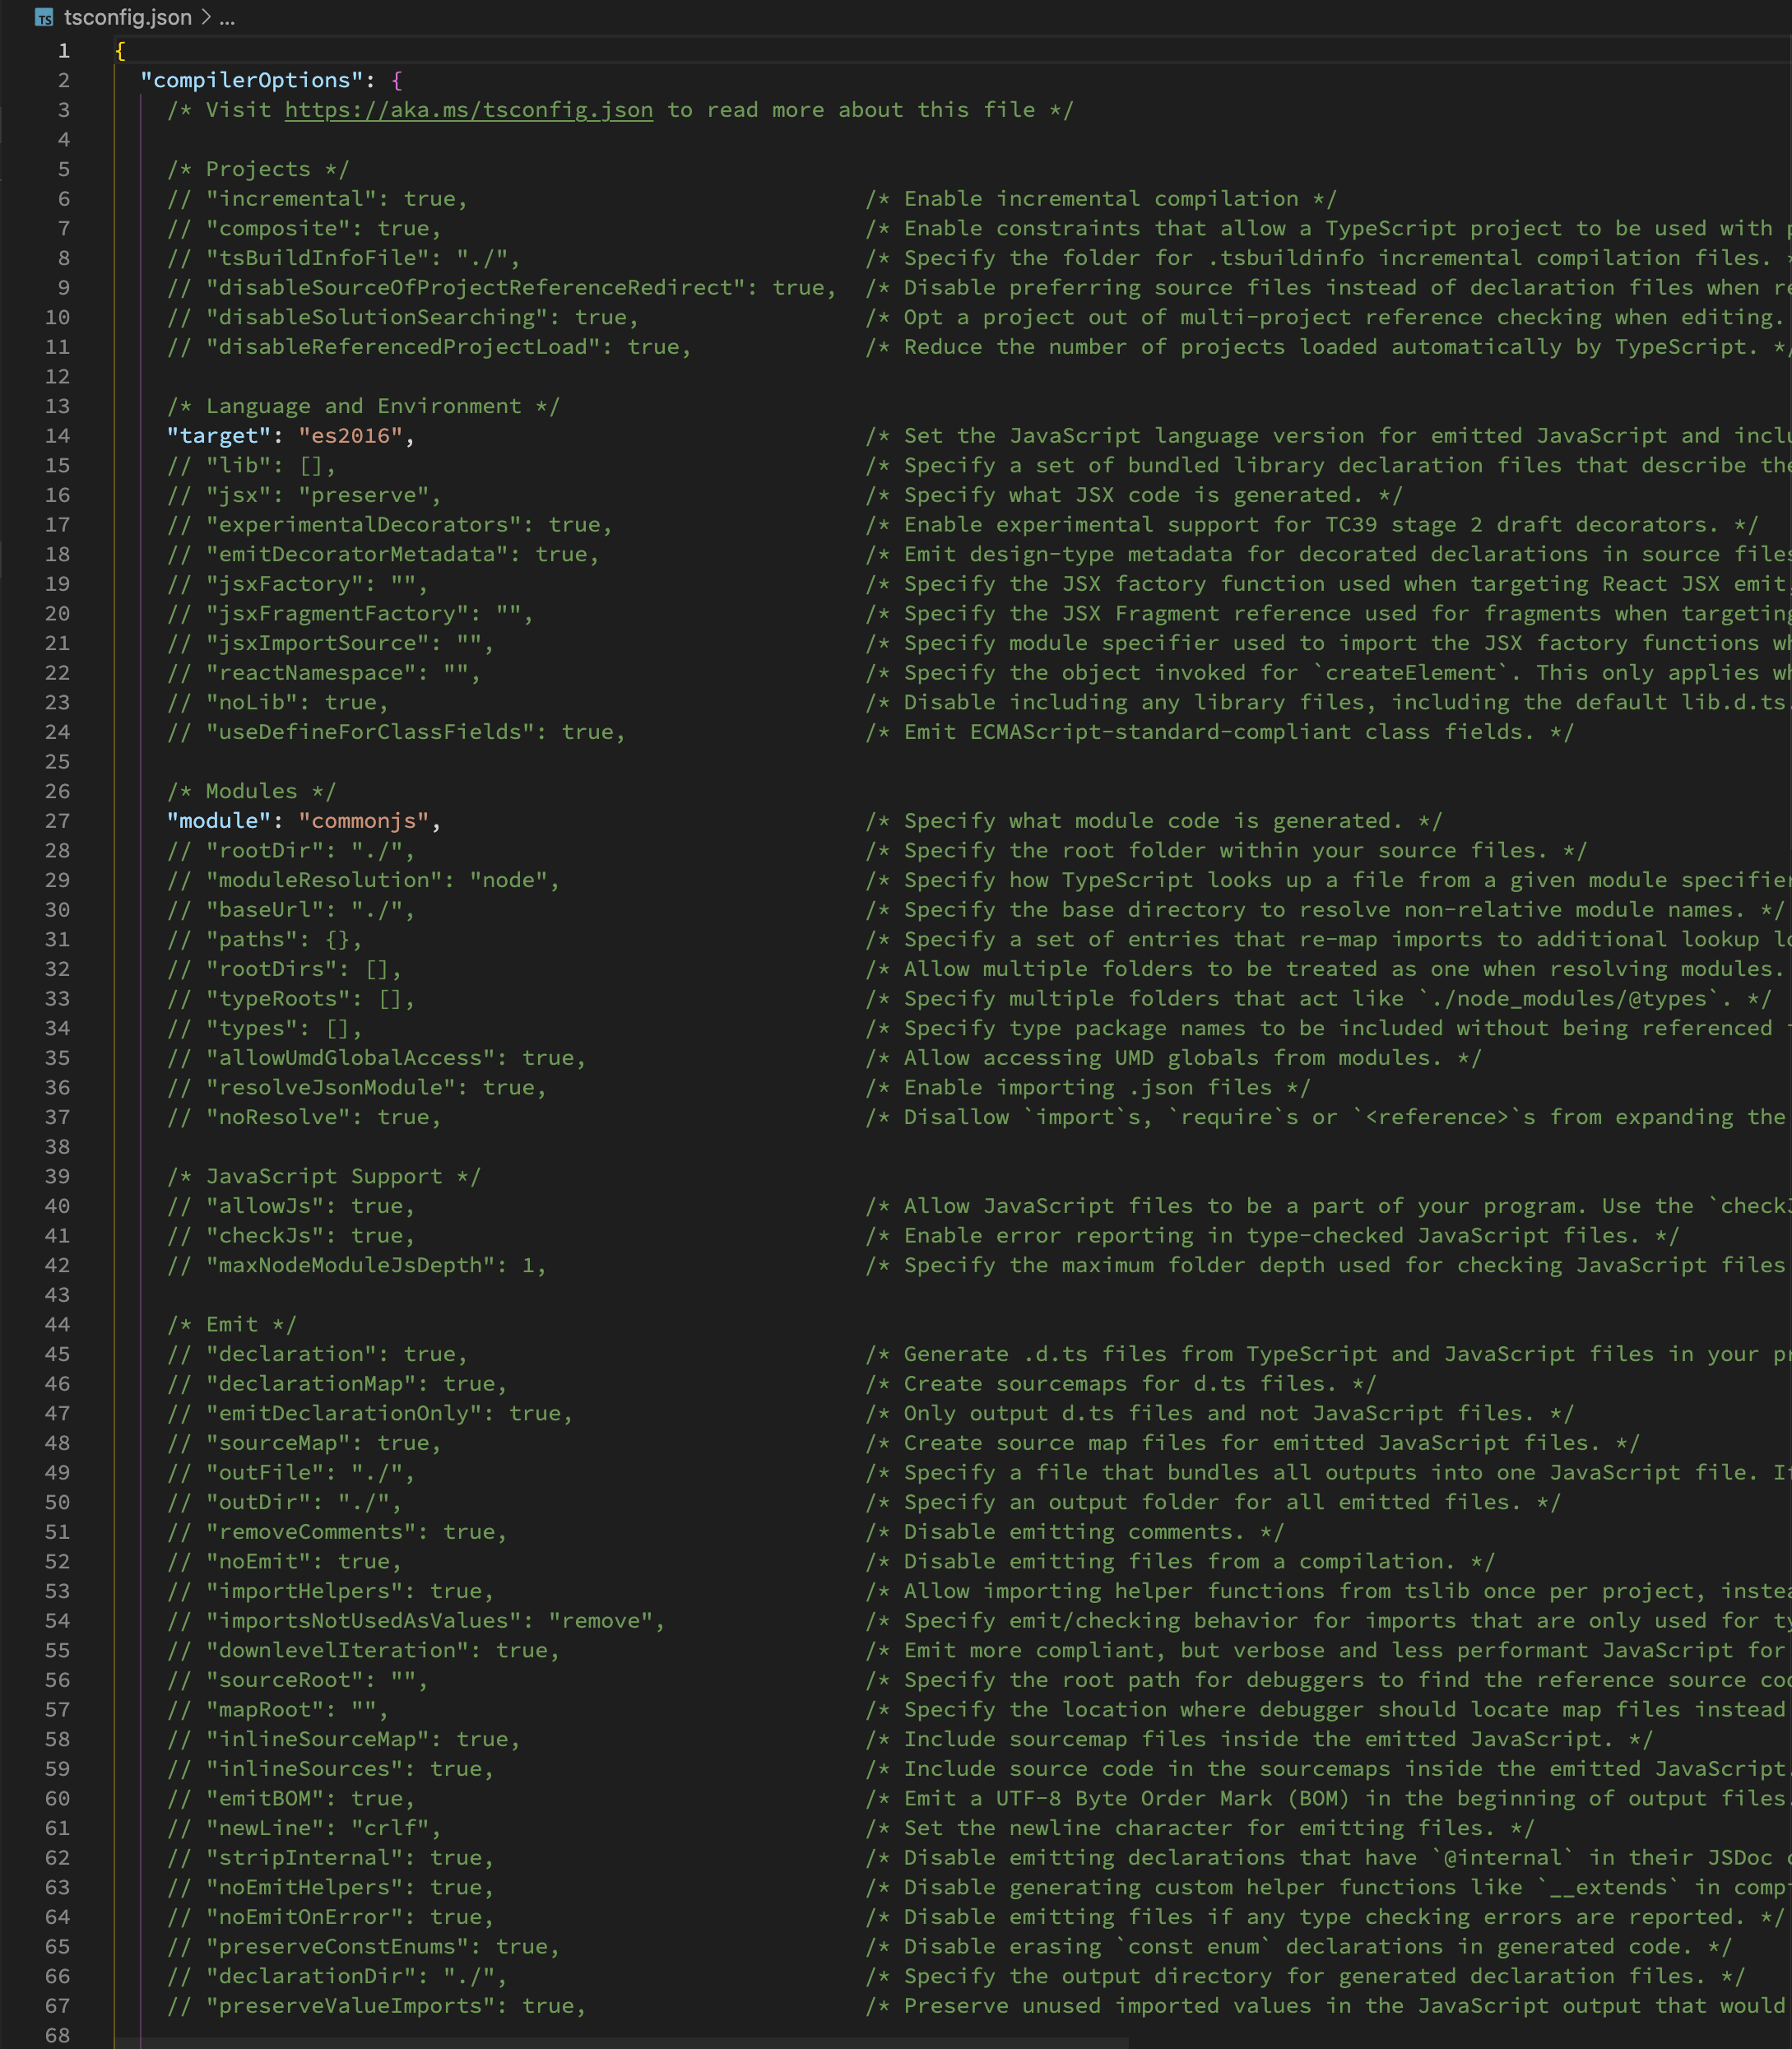
\includegraphics[width=0.8\maxwidth]{./images/02-create-react-app/typescript04.png}%
\reviewimagecaption{作成されたtsconfig.json}
\label{image:02-create-react-app:typescript04}
\end{reviewimage}

\clearpage


TypeScriptコンパイラのオプションは、
こちら\footnote{\url{https://www.typescriptlang.org/docs/handbook/tsconfig-json.html}}
で確認できます。

\vspace*{\baselineskip}

TypeScript開発元のMicrosoftは、Reactへ導入した
「tsconfig.json」のお勧め\footnote{\url{https://github.com/Microsoft/TypeScript-React-Starter/blob/master/tsconfig.json}}
を以下のようにしています。

\def\startercodeblockfontsize{}
\begin{starterprogram}[]{Microsoftお勧めReact下のtsconfig.json}\seqsplit{  \{
    "compilerOptions": \{
      "outDir": "build/dist",
      "module": "commonjs",
      "target": "es5",
      "lib": ["es6", "dom"],
      "sourceMap": true,
      "allowJs": true,
      "jsx": "react",
      "moduleResolution": "node",
      "rootDir": "src",
      "noImplicitReturns": true,
      "noImplicitThis": true,
      "noImplicitAny": true,
      "strictNullChecks": true
    \},
    "exclude": [
      "node\textunderscore{}modules",
      "build",
      "scripts",
      "acceptance{-}tests",
      "webpack",
      "jest",
      "src/setupTests.ts"
    ],
    "types": [
      "typePatches"
    ]
  \}}\end{starterprogram}

Microsoftお勧めの設定に修正したものが、こちらです。コメントアウトされているものは削除しています。

\def\startercodeblockfontsize{}
\begin{starterprogram}[]{修正後のtsconfig.json}  \{
    "compilerOptions": \{
      "target": "es5",
      "lib": [
        "es6",
        "dom"
      ],
      "jsx": "react",
      "module": "commonjs",
      "rootDir": "src",
      "outDir": "public",
      "esModuleInterop": true,
      "forceConsistentCasingInFileNames": true,
      "strict": true,
      "skipLibCheck": true
    \},
    "exclude": ["node\textunderscore{}modules", "public", "webpack"]
  \}
\end{starterprogram}

TypeScriptは、ファイル拡張子が

\begin{starteritemize}
\item .js {-}{-}{-}\textgreater{} .ts
\item .jsx {-}{-}\textgreater{} .tsx
\end{starteritemize}

となるため、「webpack.common.js」の「entry」のファイル名の拡張子を「.tsx」に変えます。

\def\startercodeblockfontsize{}
\begin{starterprogram}[]{webpack.common.jsの一部}\seqsplit{  const path = require('path');
  const HtmlWebpackPlugin = require('html{-}webpack{-}plugin');

  module.exports = \{
    entry: './src/index.tsx',
    output: \{
      path: path.resolve(\textunderscore{}\textunderscore{}dirname, 'public'),
      assetModuleFilename: 'images/[name][ext][query]',
      clean: true,
    \},}\end{starterprogram}

プロジェクト内のファイル名も変更します。

\begin{starteritemize}
\item 「src/index.js」{-}{-}{-}\textgreater{} 「src/index.tsx」
\item 「src/components/App.jsx」 {-}{-}\textgreater{} 「src/components/App.tsx」
\end{starteritemize}

次に、使用するライブラリの型定義をインストールします。
ライブラリによっては自身が型定義を持っている場合もありますし、
有志で作成された型定義ファイルは、npmリポジトリの「@types/」に
ある場合もあります。

\vspace*{\baselineskip}

使用するReact、Node.jsの型定義ファイルは、「@types/」以下にありますので
インストールします。

\def\startercodeblockfontsize{}
\begin{starterterminal}[]{React、Node.jsの型定義のインストール}\seqsplit{ \textgreater{} npm install {-}D @types/node @types/react @types/react{-}dom}\end{starterterminal}

型定義のインストールが完了しても、「App.tsx」で

\begin{starteritemize}
\item lodashの型定義がない
\item yaruo.pngの型定義がない
\end{starteritemize}

と、エラーが表示されています。

\begin{reviewimage}%%typescript02
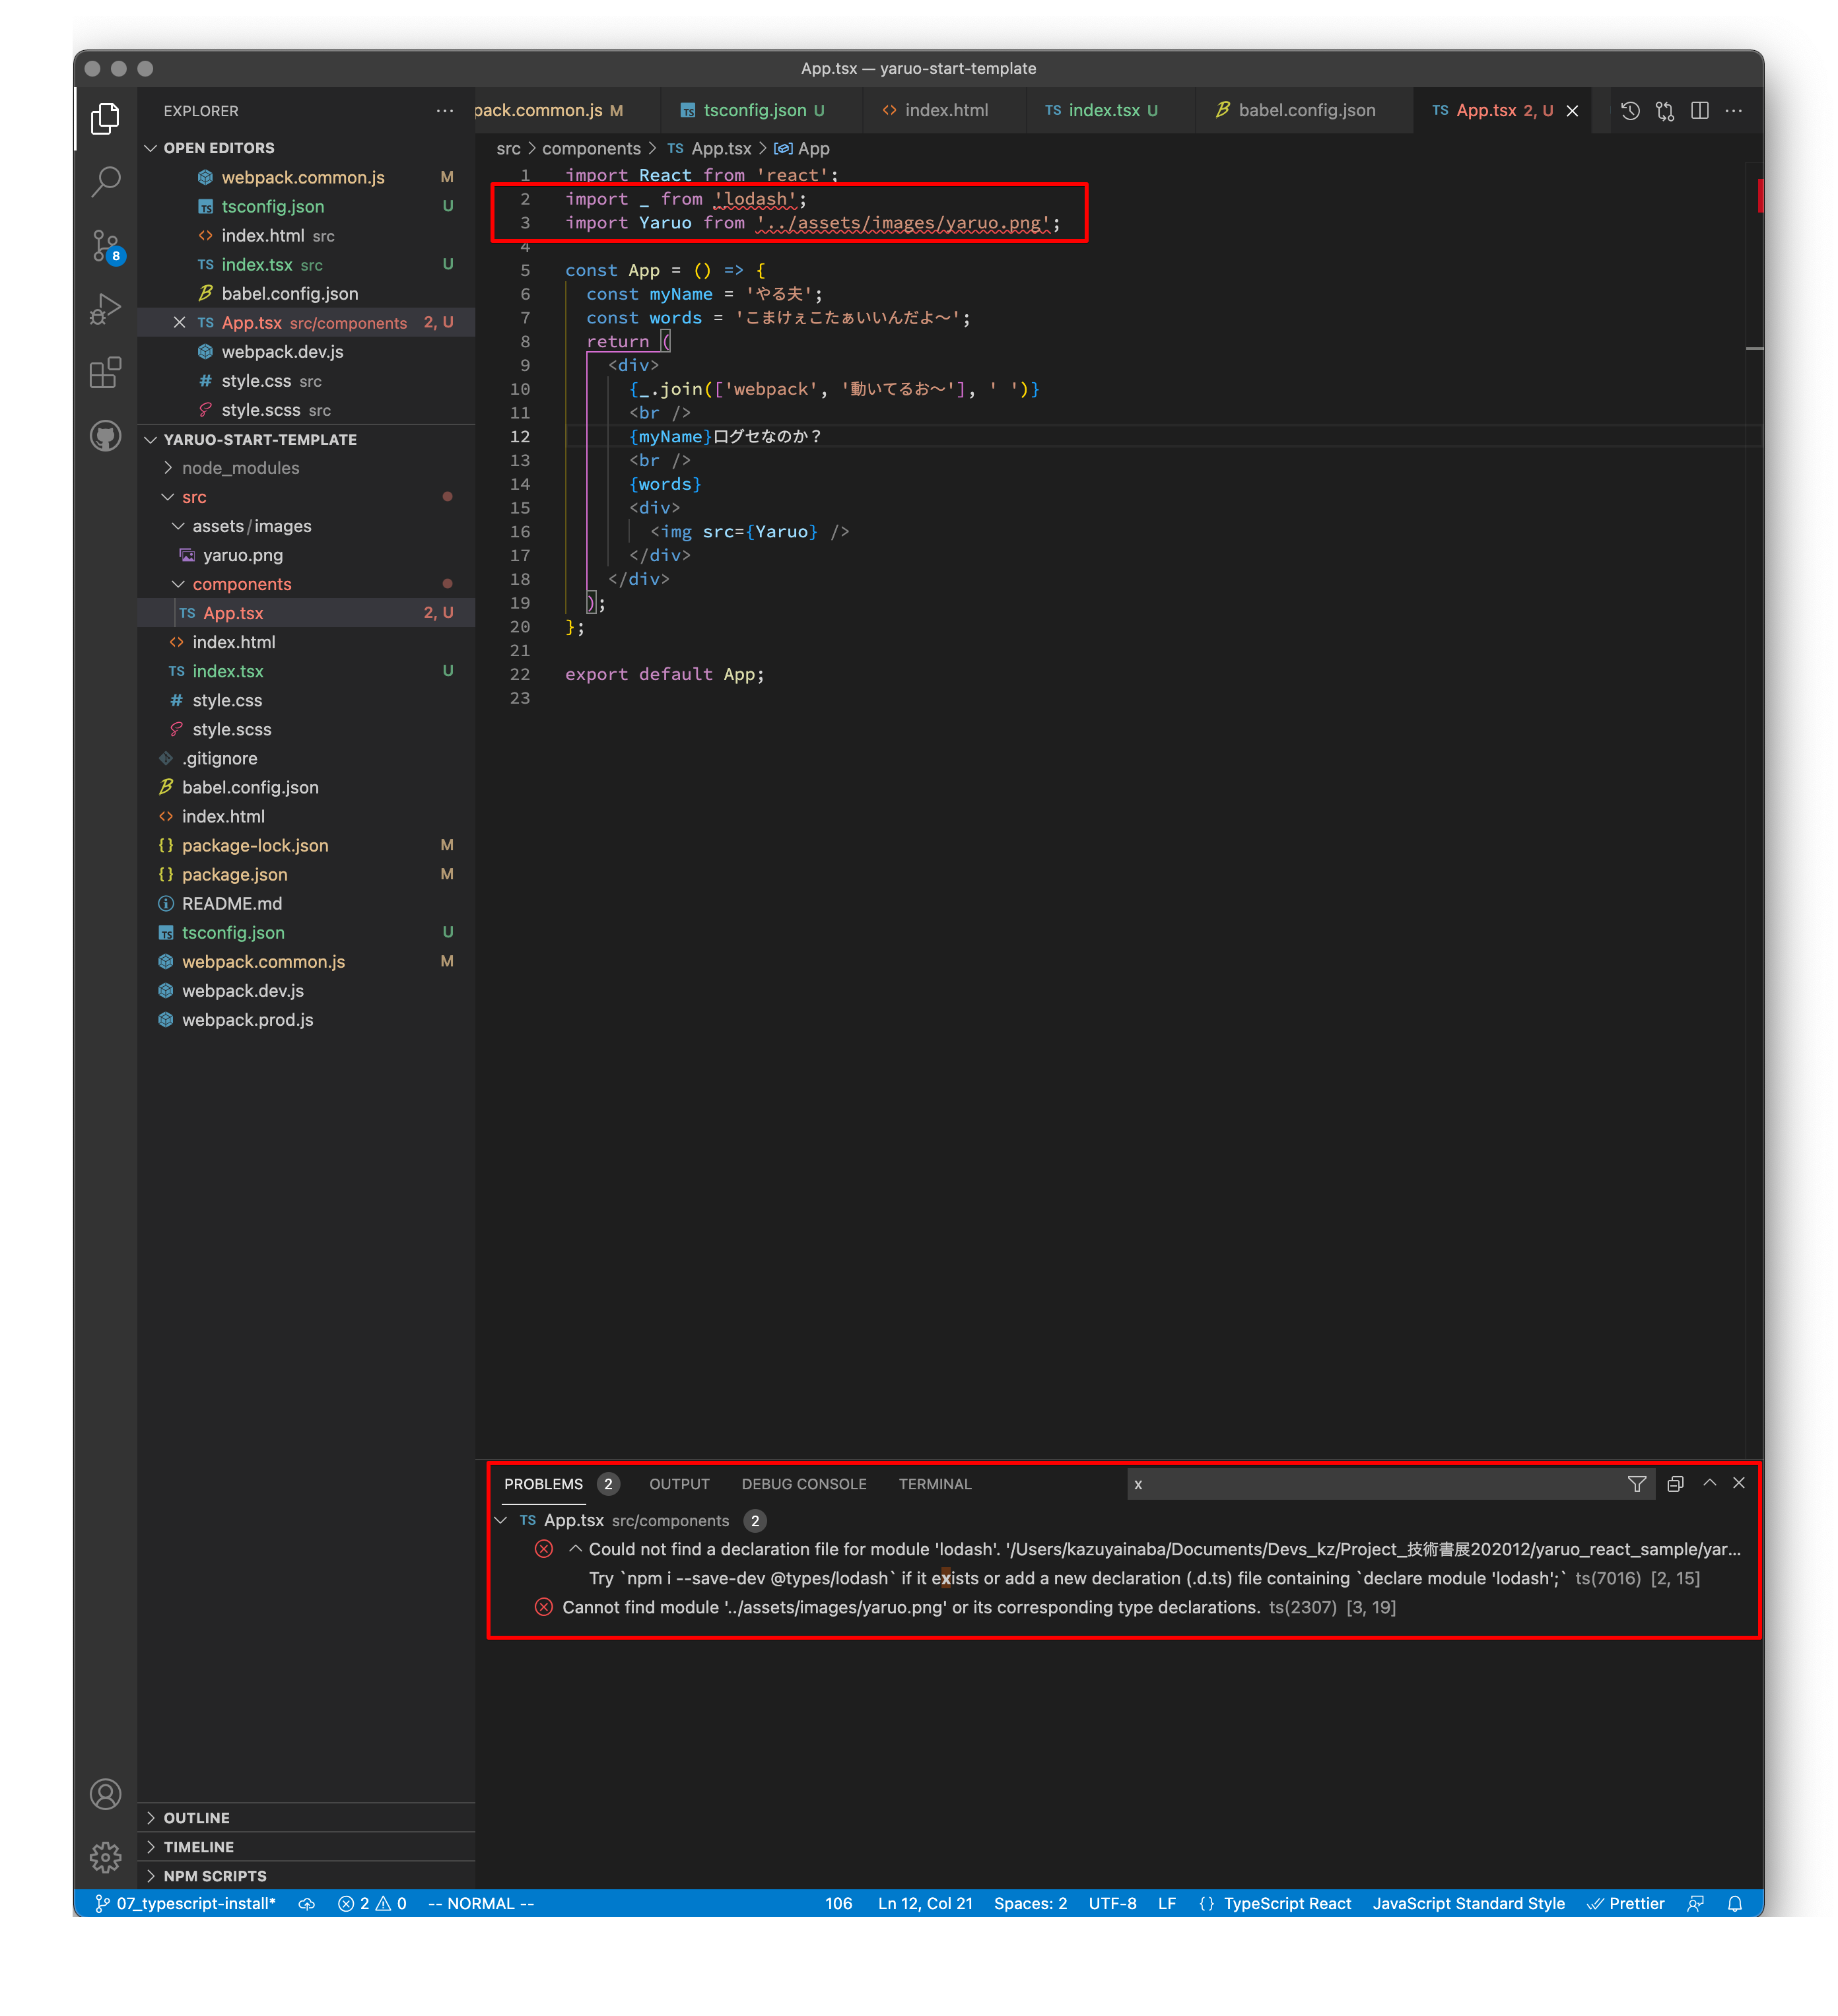
\includegraphics[width=0.7\maxwidth]{./images/02-create-react-app/typescript02.png}%
\reviewimagecaption{App.tsxでエラー表示}
\label{image:02-create-react-app:typescript02}
\end{reviewimage}

\clearpage


「lodash」の型定義はインストールすればエラーが消えますが、今後「lodash」は使わないので
アンインストールし、該当コードも削除します。

\def\startercodeblockfontsize{}
\begin{starterterminal}[]{lodashのアンインストール}\seqsplit{ \textgreater{} npm uninstall lodash}\end{starterterminal}

「png」については、プロジェクト用の型定義ファイルを作成します。

\vspace*{\baselineskip}

「src/types/index.d.ts」を作成し、以下のように記入します。

\def\startercodeblockfontsize{}
\begin{starterprogram}[]{src/types/index.d.ts}\seqsplit{declare module '*.png'}\end{starterprogram}

作成したファイルを「tsconfig.json」に型定義ファイルの位置を追加します。

\def\startercodeblockfontsize{}
\begin{starterprogram}[]{tsconfig.json}\seqsplit{  "compilerOptions": \{
    "typeRoots": [
      "types"
    ]
  \}}\end{starterprogram}

動作確認を行います。

\def\startercodeblockfontsize{}
\begin{starterterminal}[]{動作確認}\seqsplit{ \textgreater{} npm run start}\end{starterterminal}

lodash部分のコードが削除されたトップページを表示します。

\begin{reviewimage}%%typescript03
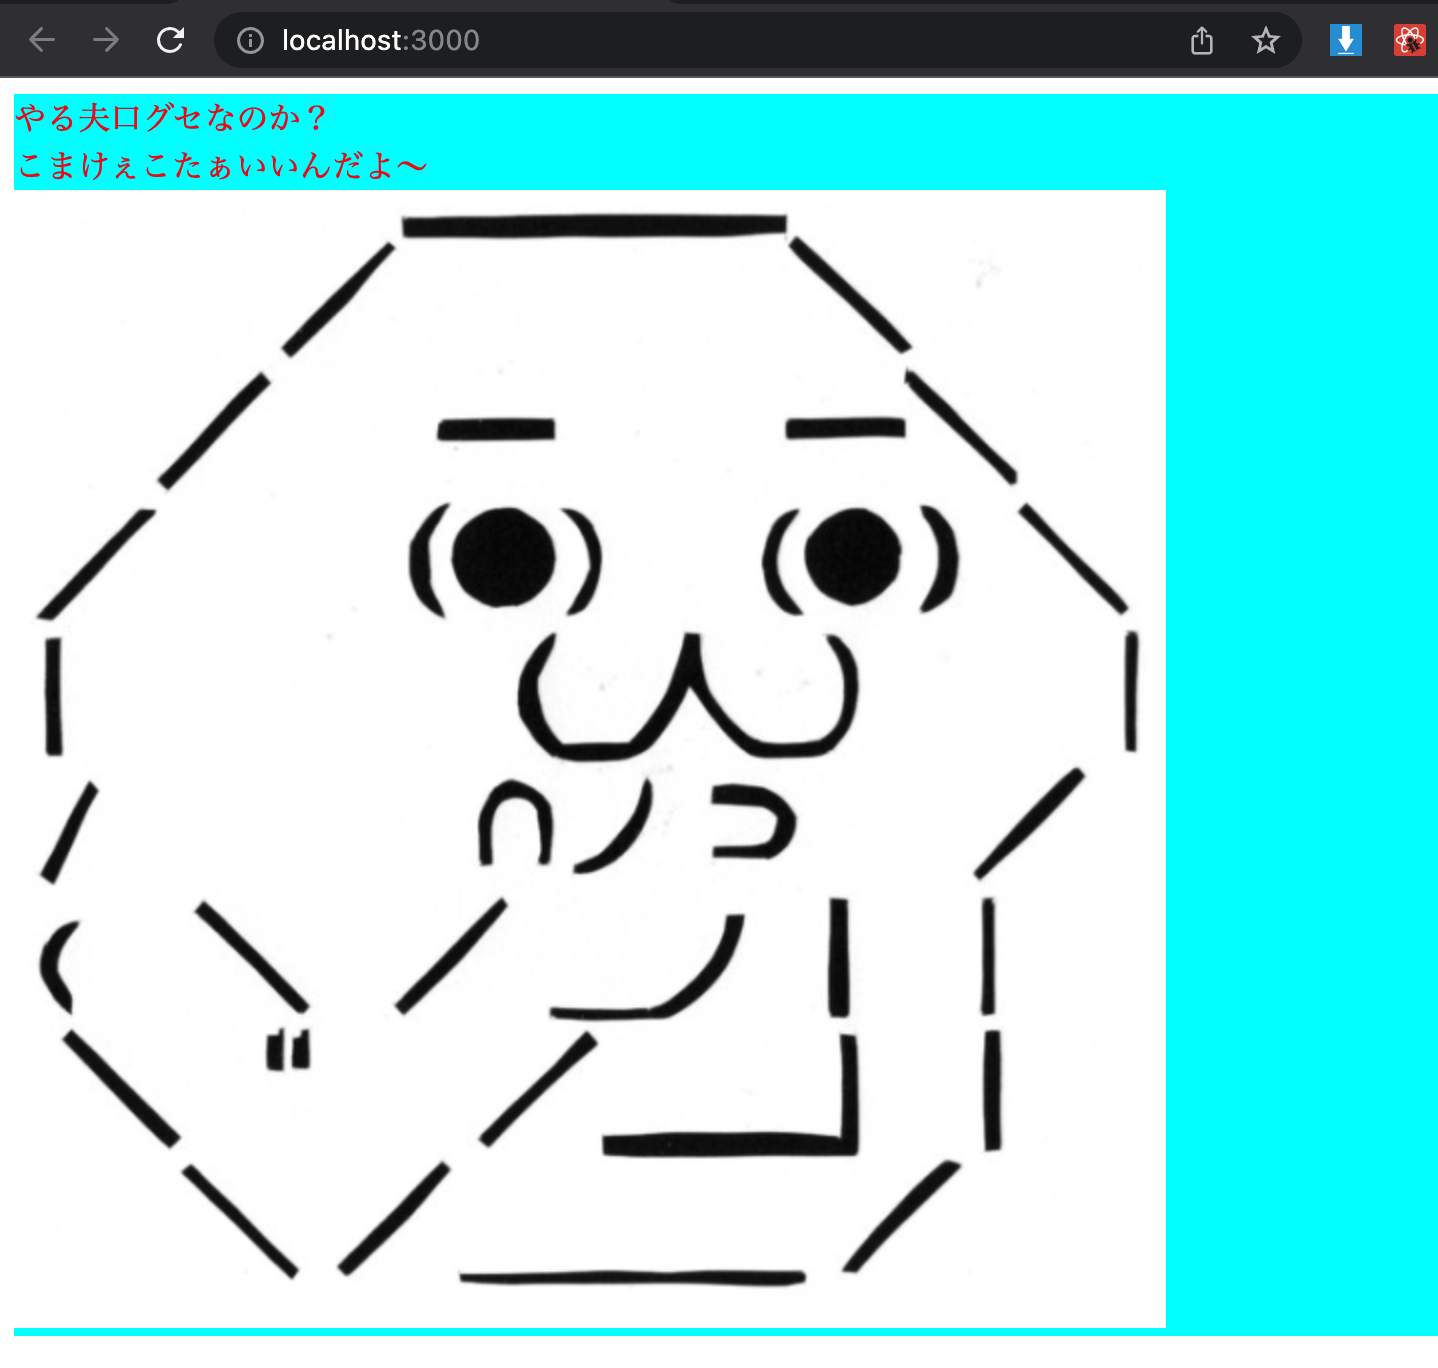
\includegraphics[width=0.6\maxwidth]{./images/02-create-react-app/typescript03.png}%
\reviewimagecaption{TypeScript導入後動作確認}
\label{image:02-create-react-app:typescript03}
\end{reviewimage}

\clearpage

\begin{starternote}[]{}

ここまでの内容は、GitHub上で、以下のコマンドでクローンできます。

\def\startercodeblockfontsize{}
\begin{starterterminal}[]{GitHub}\seqsplit{\textgreater{} git clone {-}b 07\textunderscore{}typescript{-}install https://github.com/yaruo{-}react{-}redux/yaruo{-}start{-}template.git}\end{starterterminal}
\end{starternote}

\section{eslint、prettierとは?}
\keeplastskip{
  \label{sec:2-3}
  \label{sec-03lint}
  \par\nobreak
}

「lint」は、C言語用のコンパイラよりも詳細で厳密なチェックを行うプログラムです。
コンパイル前にコードをチェックするために使われます。

\vspace*{\baselineskip}

それが、いつしかコードをチェック・解析することを「lint」、lintを行うプログラムをlinterと呼ぶようになったそうです。

\vspace*{\baselineskip}

JavaScript(ECMAScript)用のlinterが、「eslint」になります。もちろん、Java、HTML、Pythonなどにもlinterがあります。

\vspace*{\baselineskip}

「eslint」は、設定ファイルで指定されたルールと違うコードの書き方をしている部分を指摘してくれます。
その指定されたルールとは、たいていの場合にはJavaScriptに詳しい人達が決めたもので、良く使われるものは、かの有名なAirBnBの開発チームのものです。
もちろん、ルールは改変・追加もできます。

\vspace*{\baselineskip}

チェックしてくれるのは、たとえば、

\begin{starteritemize}
\item constで宣言している変数への代入
\item 未定義の変数やモジュールの使用
\item 分割代入の使用を推奨
\end{starteritemize}

などがありますが、何をチェックするのかは、チーム毎、プロジェクト毎に自由に決めることができます。

\vspace*{\baselineskip}

「prettier」は、コードを整形(インデント、改行など)してくれるツールです。
実は、eslintでもコード整形はできるのですが、コード整形はprettierの方が優れいます。

\vspace*{\baselineskip}

そのために、

\begin{starteritemize}
\item コードチェックは、eslint
\item コード整形は、prettier
\end{starteritemize}

と、得意なものに任せます。

\subsection{eslint、prettierのインストール}
\keeplastskip{
  \label{sec:2-3-1}
  \label{sec-03eslint}
  \par\nobreak
}

\subsubsection*{eslintのパッケージ追加と設定}
\keeplastskip{
  \label{sec:2-3-1-1}
  \label{sec-03eslint-install}
  \par\nobreak
}
\begin{starternote}[]{create{-}react{-}appで作成したプロジェクト}

「create{-}react{-}app」を使用して作成したスタートアッププロジェクトには、eslintは導入済みです。

\vspace*{\baselineskip}

追加のパッケージ、設定については、本章の後半で解説しています。

\end{starternote}

ターミナルに以下のように「eslint {-}{-}init」と初期化コマンドを入力します。
「eslint」が未インストール状態でしたら、「eslint」をインストールするのか問われます。

\def\startercodeblockfontsize{}
\begin{starterterminal}[]{eslintの初期化}\seqsplit{\textdollar{} npx eslint {-}{-}init
Need to install the following packages:
  eslint
Ok to proceed? (y) y}\end{starterterminal}

「y」を入力しエンターキーを押すと「eslint」がインストールされ、設定ファイルを作成するための質問が始まります。

\vspace*{\baselineskip}

「?」が行頭にある質問と選択枝が表示されますので、カーソルキーで選択枝を選びエンターキーで次ぎの質問に移ります。

\def\startercodeblockfontsize{}
\begin{starterterminal}[]{eslintの質問に答える}\seqsplit{  ? How would you like to use ESLint? …
    To check syntax only            
  \textgreater{} To check syntax and find problems    {\reviewballoon{選択したものに > が表示される}}
    To check syntax, find problems, and enforce code style}\end{starterterminal}

最後の質問に答えると必要なパッケージをインストールするか尋ねられますので「Yes」と答えてます。

\def\startercodeblockfontsize{}
\begin{starterterminal}[]{eslintへの答え}\seqsplit{  ✔ How would you like to use ESLint? · style
  ✔ What type of modules does your project use? · esm
  ✔ Which framework does your project use? · react
  ✔ Does your project use TypeScript? · No / Yes  {\reviewballoon{Yesを選択}}
  ✔ Where does your code run? · browser
  ✔ How would you like to define a style for your project? · guide
  ✔ Which style guide do you want to follow? · airbnb
  ✔ What format do you want your config file to be in? · JavaScript
  Checking peerDependencies of eslint{-}config{-}airbnb@latest
  Local ESLint installation not found.
  The config that you've selected requires the following dependencies:

  eslint{-}plugin{-}react@\textasciicircum{}7.27.1 @typescript{-}eslint/eslint{-}plugin@latest eslint{-}config{-}airbnb@latest eslint@\textasciicircum{}7.32.0 \textbar{}\textbar{} \textasciicircum{}8.2.0 eslint{-}plugin{-}import@\textasciicircum{}2.25.3 eslint{-}plugin{-}jsx{-}a11y@\textasciicircum{}6.5.1 eslint{-}plugin{-}react{-}hooks@\textasciicircum{}4.3.0 @typescript{-}eslint/parser@latest
  ? Would you like to install them now with npm? › No / Yes {\reviewballoon{Yesを選択}}}\end{starterterminal}
\def\startercodeblockfontsize{}
\begin{starterprogram}[]{package.jsonにeslint関連のパッケージがインストールされました。}\seqsplit{  "devDependencies": \{
    "@typescript{-}eslint/eslint{-}plugin": "\textasciicircum{}5.8.0",
    "@typescript{-}eslint/parser": "\textasciicircum{}5.8.0",
    "@webpack{-}cli/generators": "\textasciicircum{}2.4.1",
    "eslint": "\textasciicircum{}8.5.0",
    "eslint{-}config{-}airbnb": "\textasciicircum{}19.0.2",
    "eslint{-}plugin{-}import": "\textasciicircum{}2.25.3",
    "eslint{-}plugin{-}jsx{-}a11y": "\textasciicircum{}6.5.1",
    "eslint{-}plugin{-}react": "\textasciicircum{}7.28.0",
    "eslint{-}plugin{-}react{-}hooks": "\textasciicircum{}4.3.0",
  \}}\end{starterprogram}

また、eslintの設定ファイル「.eslintrc.js」が作成されています。

\def\startercodeblockfontsize{}
\begin{starterprogram}[]{.eslint.js}\seqsplit{  module.exports = \{
      "env": \{
          "browser": true,
          "es2021": true
      \},
      "extends": [
          "plugin:react/recommended",
          "airbnb"
      ],
      "parser": "@typescript{-}eslint/parser",
      "parserOptions": \{
          "ecmaFeatures": \{
              "jsx": true
          \},
          "ecmaVersion": 13,
          "sourceType": "module"
      \},
      "plugins": [
          "react",
          "@typescript{-}eslint"
      ],
      "rules": \{
      \}
  \};}\end{starterprogram}

設定ファイル「.eslintrc.js」で、どのようなルールが適用されるのかを確認します。
適用されるルールが、「current\textunderscore{}rules.txt」に書き出されます。

\vspace*{\baselineskip}

書き出されたルールは、ルール名に適用方法\{"off(適用しない)","warn(警告)","error(エラー)"\}が記されています。
表記は、\{0,1,2\}の数字で表示される場合もあります。
同じルールがあった場合には、後から読み込まれたルールに上書きされます。
個別に上書きしたいものは「.eslintrc.js」ファイルの「rules」セクションに追加します。

\def\startercodeblockfontsize{}
\begin{starterterminal}[]{eslint設定で適用されるルール}\seqsplit{\textdollar{} npx eslint {-}{-}print{-}config .eslintrc.js \textgreater{} current\textunderscore{}rules.txt}\end{starterterminal}

「eslint {-}{-}init」時にインストールされたルールが適用されるように「extends」に追加します。

\vspace*{\baselineskip}

次に、TypeScriptもチェックできるようにルールを追加します。「plugin:」の下3行を追加しました。

\def\startercodeblockfontsize{}
\begin{starterprogram}[]{.eslintrc.jsのextends部分}\seqsplit{  "extends": [
  'plugin:react/recommended',
  'airbnb',
  'airbnb/hooks',
  'plugin:@typescript{-}eslint/recommended',
  'plugin:@typescript{-}eslint/recommended{-}requiring{-}type{-}checking',
  'plugin:import/recommended',
  'plugin:import/typescript',
  ],}\end{starterprogram}

再度、ルールを出力すると適用されるルールがずいぶん増えているのが分かります。

TypeScript用ルールを追加しましたので、「parserOptions」を以下のように変更する。

\def\startercodeblockfontsize{}
\begin{starterprogram}[]{.eslintrc.jsのparserOptions部分}\seqsplit{  "parserOptions": \{
    "ecmaFeatures": \{
        "jsx": true
    \},
    "ecmaVersion": 12,
    "sourceType": "module",
    "tsconfigRootDir": \textunderscore{}\textunderscore{}dirname,
    "project": ["./tsconfig.json"],
  \},}\end{starterprogram}

これでルールの適用は完了しましたが、都合の悪いルールには設定ファイルでルールの上書をします。

\vspace*{\baselineskip}

ルール「import/extensions」は、インポート宣言でnode\textunderscore{}modules以下にあるパッケージからは拡張子が不要(import aaa from 'aaa')
で、相対パスからのimportは、拡張子が必要と言うルールです。

現在はすべてがエラー、node\textunderscore{}modules下のパッケージ内の指定された拡張子は除外となっていますが、
node\textunderscore{}modules下以外でも\{js,jsx,ts,tsx\}は除外したいのでルールを追加します。

\def\startercodeblockfontsize{}
\begin{starterprogram}[]{import/extensionsの現時点}\seqsplit{  "import/extensions": [
    "error",
    "ignorePackages",
    \{
      "js": "never",
      "mjs": "never",
      "jsx": "never"
    \}
  ],}\end{starterprogram}

「react/jsx{-}filename{-}extension」は、JSXを含むファイルの拡張子を制限するルールです。

現時点では、拡張子「.jsx」に制限されていますが、拡張子「.tsx」も追加したいのでルールに追加します。

\def\startercodeblockfontsize{}
\begin{starterprogram}[]{react/jsx{-}filename{-}extentionの現時点}\seqsplit{  "react/jsx{-}filename{-}extension": [
    "error",
    \{
      "extensions": [
        ".jsx"
      ]
    \}
  ],}\end{starterprogram}

「react/react{-}in{-}jsx{-}scope」は、JSXファイルに「import React from 'react'」がない場合にはエラーにしてくれるのですが
React17からは、「import React from 'react'」を書かなくてもよくなりました。そのため、このルールをOFFにします。

\def\startercodeblockfontsize{}
\begin{starterprogram}[]{react/react{-}in{-}jsx{-}scope}\seqsplit{  "react/react{-}in{-}jsx{-}scope": [
    "error"
  ],}\end{starterprogram}

「react/function{-}component{-}definition」は、関数コンポーネントに特定の関数タイプを強制します。
現時点では、functionの使用を強制されるので、アロー関数強制に変更します。

\def\startercodeblockfontsize{}
\begin{starterprogram}[]{react/function{-}component{-}definitionの現在}\seqsplit{  "react/function{-}component{-}definition": [
    "error",
    \{
      "namedComponents": "function{-}expression",
      "unnamedComponents": "function{-}expression"
    \}
  ],}\end{starterprogram}

「no{-}void」は、void演算子を使用するとundefinedを返すため禁止してあります。
「create{-}react{-}app」で作成される「reportWebVitals.ts」でvoid使います。
文としての使用だけを可能にします。

\def\startercodeblockfontsize{}
\begin{starterprogram}[]{no{-}voidの現在}\seqsplit{  "no{-}void": [
    "error"
  ],}\end{starterprogram}

上書きしたいルールを、「.eslintrc.js」へ追加します。

\def\startercodeblockfontsize{}
\begin{starterprogram}[]{.eslintrc.jsのrulesへ追加}\seqsplit{  "rules": \{
      "import/extensions": [
          "error",
          \{
            js: "never",
            jsx: "never",
            ts: "never",
            tsx: "never",
          \},
        ],
        "react/jsx{-}filename{-}extension": [
          "error",
          \{
            extensions: [".jsx", ".tsx"],
          \},
        ],
        "react/react{-}in{-}jsx{-}scope": "off",
        "react/function{-}component{-}definition": [
          "error",
          \{
            namedComponents: "arrow{-}function",
            unnamedComponents: "arrow{-}function",
          \},
        ],
        'no{-}void': [
          'error',
          \{
            allowAsStatement: true,
          \},
        ],
  \}}\end{starterprogram}

\subsubsection*{Prettierのインストールと設定}
\keeplastskip{
  \label{sec:2-3-1-2}
  \label{sec-03prettier}
  \par\nobreak
}

ここからは、Prettierのインストールと設定をします。

\def\startercodeblockfontsize{}
\begin{starterterminal}[]{Prettierのインストール}\seqsplit{  \textgreater{} npm install {-}D prettier eslint{-}config{-}prettier}\end{starterterminal}

インストールが完了すると、package.jsonに追加されます。

\def\startercodeblockfontsize{}
\begin{starterprogram}[]{package.json}\seqsplit{  "devDependencies": \{
    "eslint{-}config{-}prettier": "\textasciicircum{}8.3.0",
    "prettier": "\textasciicircum{}2.5.1"
  \}}\end{starterprogram}

Pretterのチェックを「.eslintrc.js」へ追加します。

\def\startercodeblockfontsize{}
\begin{starterprogram}[]{.eslintrc.js}\seqsplit{  "extends": [
  'plugin:react/recommended',
  'airbnb',
  'airbnb/hooks',
  'plugin:@typescript{-}eslint/recommended',
  'plugin:@typescript{-}eslint/recommended{-}requiring{-}type{-}checking',
  'plugin:import/recommended',
  'plugin:import/typescript',
  'prettier'  {\reviewballoon{prettierを追加}}
  ],}\end{starterprogram}

pritterの設定ファイル「.prettierrc」を追加します。設定可能なオプションは、
Prettierオプション\footnote{\url{https://prettier.io/docs/en/options.html}}で確認できます。
ほぼすべてがデフォルトでも良いのですが、create{-}react{-}appがシングルクオートなので設定します。

\def\startercodeblockfontsize{}
\begin{starterprogram}[]{.prettierrc}\seqsplit{  \{
    "singleQuote": true,
    "jsxSingleQuote": true
  \}}\end{starterprogram}

eslintとprettierが衝突すると検出・修正ループに入りますので、チェックします。

\def\startercodeblockfontsize{}
\begin{starterterminal}[]{eslint、prettierの衝突検出}\seqsplit{  \textdollar{} npx eslint{-}config{-}prettier 'src/**/*.\{js,jsx,ts,tsx\}'
    No rules that are unnecessary or conflict with Prettier were found.}\end{starterterminal}

無事に衝突なしとなりました。

package.jsonにスクリプトコマンドを追加します。

\def\startercodeblockfontsize{}
\begin{starterprogram}[]{package.json}\seqsplit{"scripts": \{
  "scripts": \{
    "test": "echo \reviewbackslash{}"Error: no test specified\reviewbackslash{}" \&\& exit 1",
    "build": "webpack {-}{-}config webpack.prod.js",
    "build:dev": "webpack {-}{-}config webpack.dev.js",
    "build:prod": "webpack {-}{-}config webpack.prod.js",
    "start": "webpack serve {-}{-}config webpack.dev.js",
    "lint": "eslint 'src/**/*.\{js,jsx,ts,tsx\}'", {\reviewballoon{lint:チェック}}
    "fix": "npm run format \&\& npm run lint:fix", {\reviewballoon{fix:整形してチェックして自動修復}}
    "format": "prettier {-}{-}write 'src/**/*.\{js,jsx,ts,tsx\}'", {\reviewballoon{format:整形}}
    "lint:fix": "eslint {-}{-}fix 'src/**/*.\{js,jsx,ts,tsx\}'",  {\reviewballoon{lint:fixチェック後修復}}
  \},
\},}\end{starterprogram}

Eslint、Prettierの設定が完了しましたので、srcフォルダにある「App.tsx」を開いてみると、
ルールから外れるものは指摘されています。

\vspace*{\baselineskip}

以上で環境構築は完了なのですが、「.eslintrc.js」にてエラーが表示されています。

\begin{starterquote}

Parsing error: "parserOptions.project" has been set for @typescript{-}eslint/parser.
The file does not match your project config: .eslintrc.js.
The file must be included in at least one of the projects provided.

\end{starterquote}

このエラーは、「parserOptions.project」で「tsconfig.json」を指定していますが、
「tsconfig.json」では、「module」で「commonjs」を指定しています。

\vspace*{\baselineskip}

そのため、「eslintrc.js」ファイルが、どこからもimportされていないので警告が出ています。

\vspace*{\baselineskip}

解決策として、「eslint」の対象外とするために「.eslintignore」を作成し、「eslintrc.js」を指定します。

\def\startercodeblockfontsize{}
\begin{starterprogram}[]{.eslintignore}\seqsplit{.eslintrc.js}\end{starterprogram}

これでエラーが解消されます。

\begin{starternote}[]{}

ここまでの内容は、GitHub上で、以下のコマンドでクローンできます。

\def\startercodeblockfontsize{}
\begin{starterterminal}[]{GitHub}\seqsplit{\textgreater{} git clone {-}b 07\textunderscore{}typescript{-}install https://github.com/yaruo{-}react{-}redux/yaruo{-}start{-}template.git}\end{starterterminal}
\end{starternote}

\subsection{create{-}react{-}app作成のプロジェクトへ「eslint,prettier」を設定}
\keeplastskip{
  \label{sec:2-3-2}
  \label{sec04-cra-with-eslint}
  \par\nobreak
}

「create{-}react{-}app」で作成したプロジェクトには、下図のようにeslintが組み込まれています。

\begin{reviewimage}%%cra-eslint01
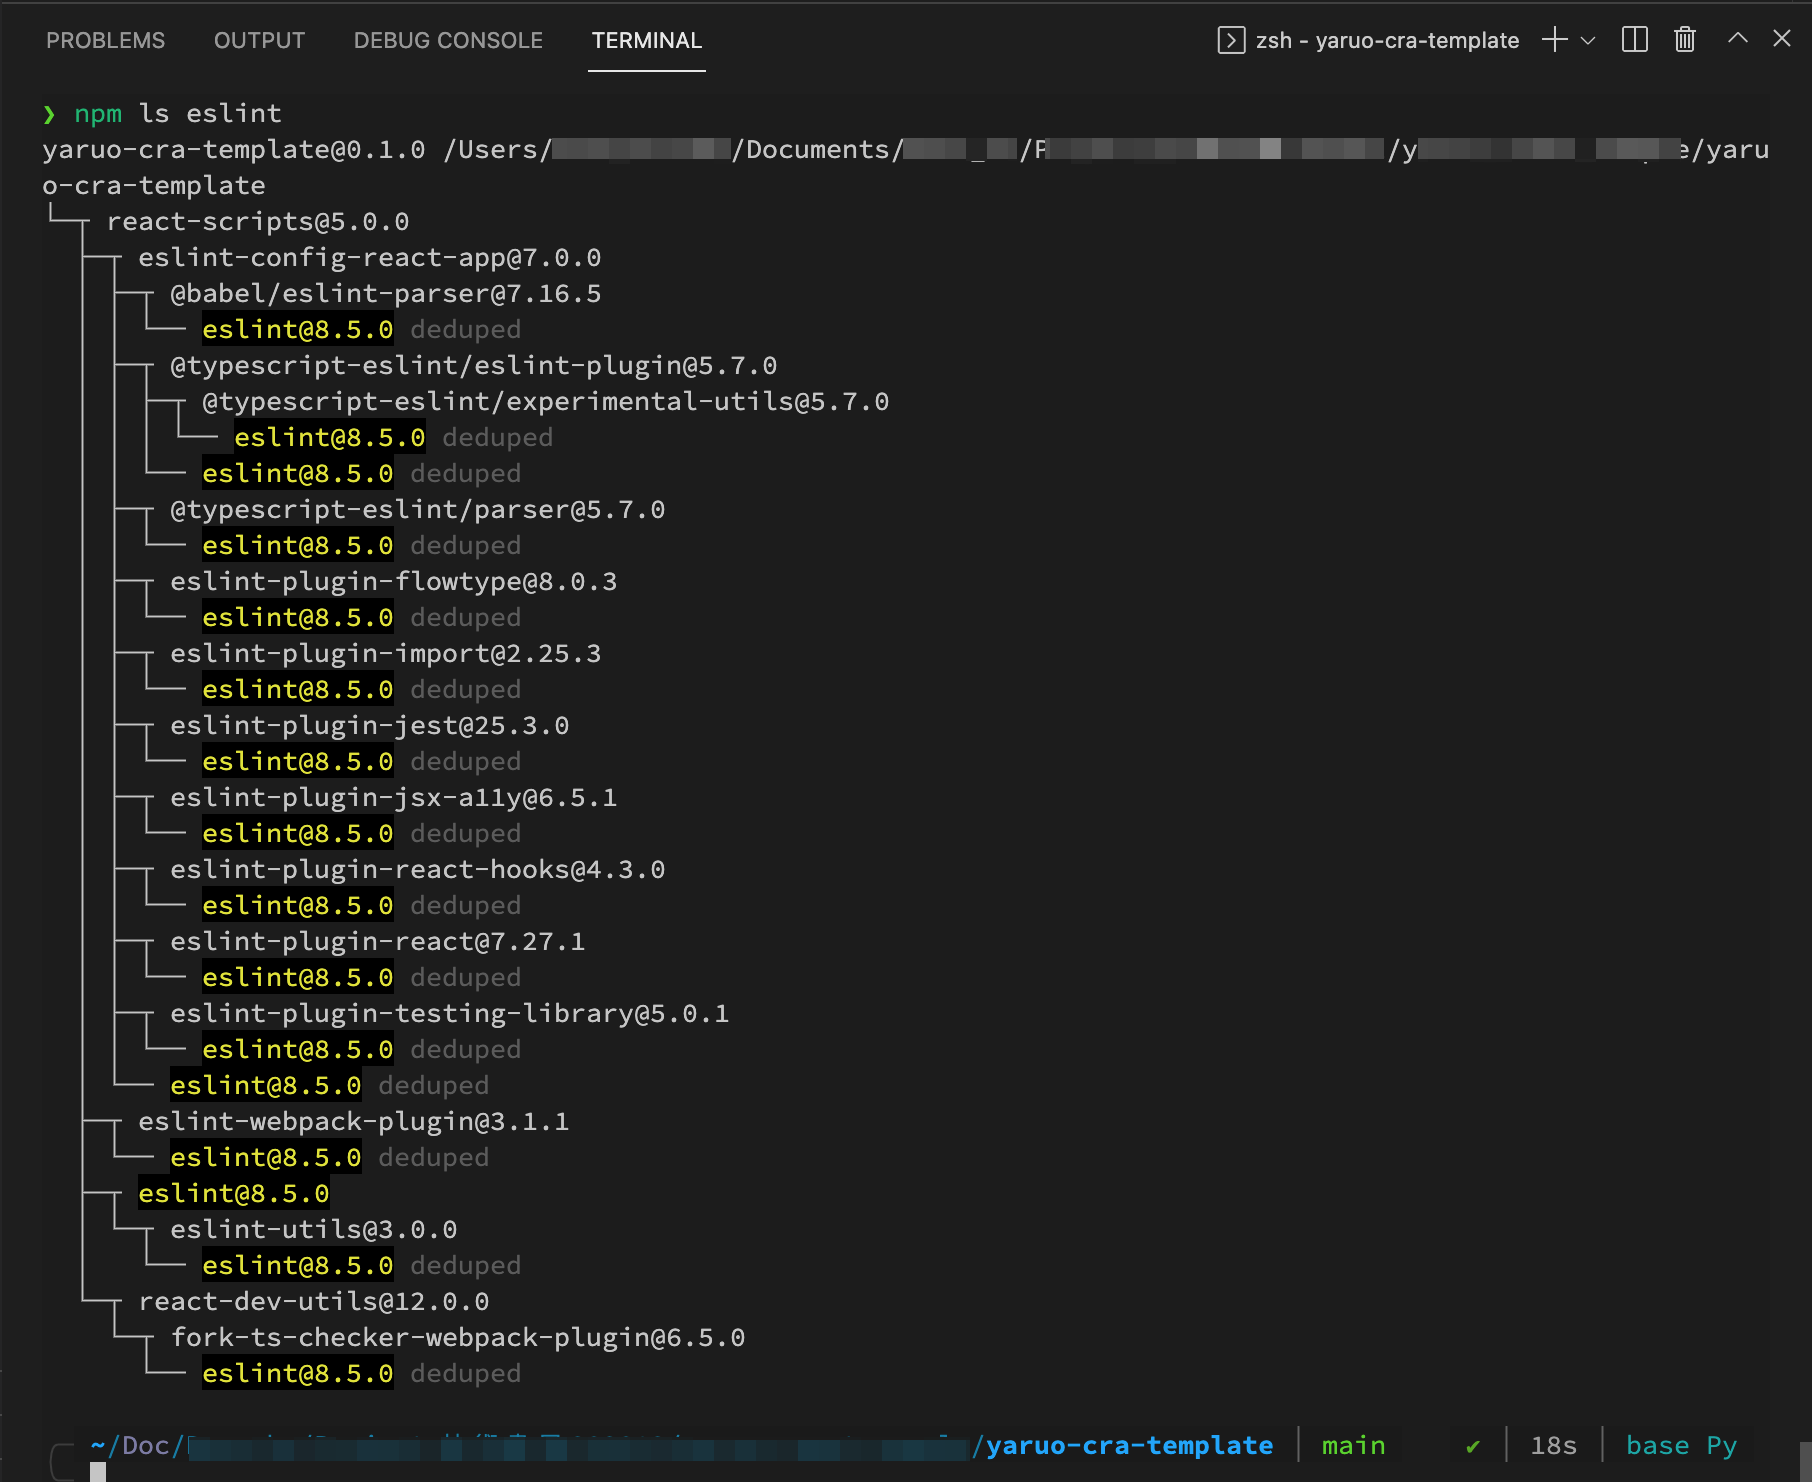
\includegraphics[width=0.8\maxwidth]{./images/02-create-react-app/cra-eslint01.png}%
\reviewimagecaption{create{-}react{-}appのeslint}
\label{image:02-create-react-app:cra-eslint01}
\end{reviewimage}

\clearpage


「npx eslint {-}{-}init」でインストールした

\begin{starteritemize}
\item eslint{-}plugin{-}react@\textasciicircum{}7.27.1
\item @typescript{-}eslint/eslint{-}plugin@latest
\item eslint{-}config{-}airbnb@latest
\item eslint@\textasciicircum{}7.32.0 \textbar{}\textbar{} \textasciicircum{}8.2.0
\item eslint{-}plugin{-}import@\textasciicircum{}2.25.3
\item eslint{-}plugin{-}jsx{-}a11y@\textasciicircum{}6.5.1
\item eslint{-}plugin{-}react{-}hooks@\textasciicircum{}4.3.0
\item @typescript{-}eslint/parser@latest
\end{starteritemize}

のうち、airbnb以外はインストールされています。

そのため、「eslint{-}config{-}airbnb」だけをインストールします。

\def\startercodeblockfontsize{}
\begin{starterterminal}[]{create{-}react{-}app作成プロジェクトへeslint{-}config{-}airbnbのインストール}\seqsplit{ ❯ npm install {-}D eslint{-}config{-}airbnb}\end{starterterminal}

設定ファイル「.eslintrc.js」を「ゼロからの構築」と同じものを作成します。

\def\startercodeblockfontsize{}
\begin{starterprogram}[]{.eslintrc.js}\seqsplit{  module.exports = \{
    env: \{
      browser: true,
      es2021: true,
    \},
    extends: [
      'plugin:react/recommended',
      'airbnb',
      'airbnb/hooks',
      'plugin:@typescript{-}eslint/recommended',
      'plugin:@typescript{-}eslint/recommended{-}requiring{-}type{-}checking',
      'plugin:import/recommended',
      'plugin:import/typescript',
      'prettier',
    ],
    parser: '@typescript{-}eslint/parser',
    parserOptions: \{
      ecmaFeatures: \{
        jsx: true,
      \},
      ecmaVersion: 13,
      sourceType: 'module',
      tsconfigRootDir: \textunderscore{}\textunderscore{}dirname,
      project: ['./tsconfig.json'],
    \},
    plugins: ['react', '@typescript{-}eslint'],
    rules: \{
      'import/extensions': [
        'error',
        \{
          js: 'never',
          jsx: 'never',
          ts: 'never',
          tsx: 'never',
        \},
      ],
      'react/jsx{-}filename{-}extension': [
        'error',
        \{
          extensions: ['.jsx', '.tsx'],
        \},
      ],
      'react/react{-}in{-}jsx{-}scope': 'off',
      'react/function{-}component{-}definition': [
        'error',
        \{
          namedComponents: 'arrow{-}function',
          unnamedComponents: 'arrow{-}function',
        \},
      ],
    \},
  \};
}\end{starterprogram}

Prettierはインストールされていないためインストールします。

\def\startercodeblockfontsize{}
\begin{starterterminal}[]{create{-}react{-}app作成プロジェクトへprettierのインストール}\seqsplit{ \textgreater{} npm install {-}D prettier eslint{-}config{-}prettier}\end{starterterminal}

「.eslintignore」、「.prettierrc」を作成します。

\def\startercodeblockfontsize{}
\begin{starterprogram}[]{.eslintignore}\seqsplit{.eslintrc.js}\end{starterprogram}
\def\startercodeblockfontsize{}
\begin{starterprogram}[]{.prettierrc}\seqsplit{  \{
    "singleQuote": true,
    "jsxSingleQuote": true
  \}}\end{starterprogram}

「package.json」にある「eslint」の設定を削除します。

\def\startercodeblockfontsize{}
\begin{starterprogram}[]{package.jsonのeslint設定を削除}\seqsplit{  "eslintConfig": \{
    "extends": [
      "react{-}app",
      "react{-}app/jest"
    ]  \},}\end{starterprogram}

最後に、「package.json」にスクリプトを追加し、eslint、prettierが動作するようにします。

\def\startercodeblockfontsize{}
\begin{starterprogram}[]{package.json}\seqsplit{  "scripts": \{
    "start": "react{-}scripts start",
    "build": "react{-}scripts build",
    "test": "react{-}scripts test",
    "eject": "react{-}scripts eject",
    "lint": "eslint 'src/**/*.\{js,jsx,ts,tsx\}'",
    "fix": "npm run format \&\& npm run lint:fix",
    "format": "prettier {-}{-}write 'src/**/*.\{js,jsx,ts,tsx\}'",
    "lint:fix": "eslint {-}{-}fix 'src/**/*.\{js,jsx,ts,tsx\}'"
  \},}\end{starterprogram}

以上で、「create{-}react{-}app」で作成したプロジェクトに追加でairbnbのチェックを追加できました。

\section{eslint、prettierの指摘を修正}
\keeplastskip{
  \label{sec:2-4}
  \label{sec-04fix}
  \par\nobreak
}

ESlint、Prettierは指摘するだけではなく、修正案の提示・修正(できるものだけですが...)までしてくれます。

\vspace*{\baselineskip}

VSCodeにPrettier拡張機能を追加してあれば、
以下のように、VSCode側で設定すると、ファイルを保存する度に自動で修正をいれることもできます。

\vspace*{\baselineskip}

私は、修正を自分のタイミングで行いたいのでVSCode側の設定は行っていません。

\vspace*{\baselineskip}

もし、VSCode側の設定をする場合には、VSCodeで\\[0pt]
[File]{-}\textgreater{}[Preferences]{-}\textgreater{}[Settings]にて、以下の各項目を検索して設定するか、settings.jsonへ追加するか、
このプロジェクトのみ適用の場合は、プロジェクトフォルダ直下に「.vscode」フォルダを作成し、「settings.json」ファイルへ書き込みます。

ユーザー設定ファイルの内容が、この設定で上書きされます。

\def\startercodeblockfontsize{}
\begin{starterprogram}[]{VSCodeの設定}\seqsplit{"editor.formatOnSave": true,
"[JavaScript]": \{
  "editor.formatOnSave": false
\},
"[JavaScriptreact]": \{
  "editor.formatOnSave": false
\},
"[typescript]": \{
  "editor.formatOnSave": false
\},
"[typescriptreact]": \{
  "editor.formatOnSave": false
\},
"editor.codeActionsOnSave": \{
    "source.fixAll": true,
    "source.fixAll.eslint": false
\},
"prettier.disableLanguages": ["JavaScript", "JavaScriptreact", "typescript", "typescriptreact"],}\end{starterprogram}

VSCode上で、\\[0pt]

\begin{starteritemize}
\item 赤波線で指摘されている
\item 問題タブに表示されている
\end{starteritemize}

\vspace*{\baselineskip}

ものを修正します。

\vspace*{\baselineskip}

まずは、App.tsxファイルを修正します。

\vspace*{\baselineskip}

エラー内容は、「Functionコンポーネントは、arrow関数にしなさい。」とのことで、
これは、rulesに追加したためです。

\begin{reviewimage}%%cra-fix_app_tsx
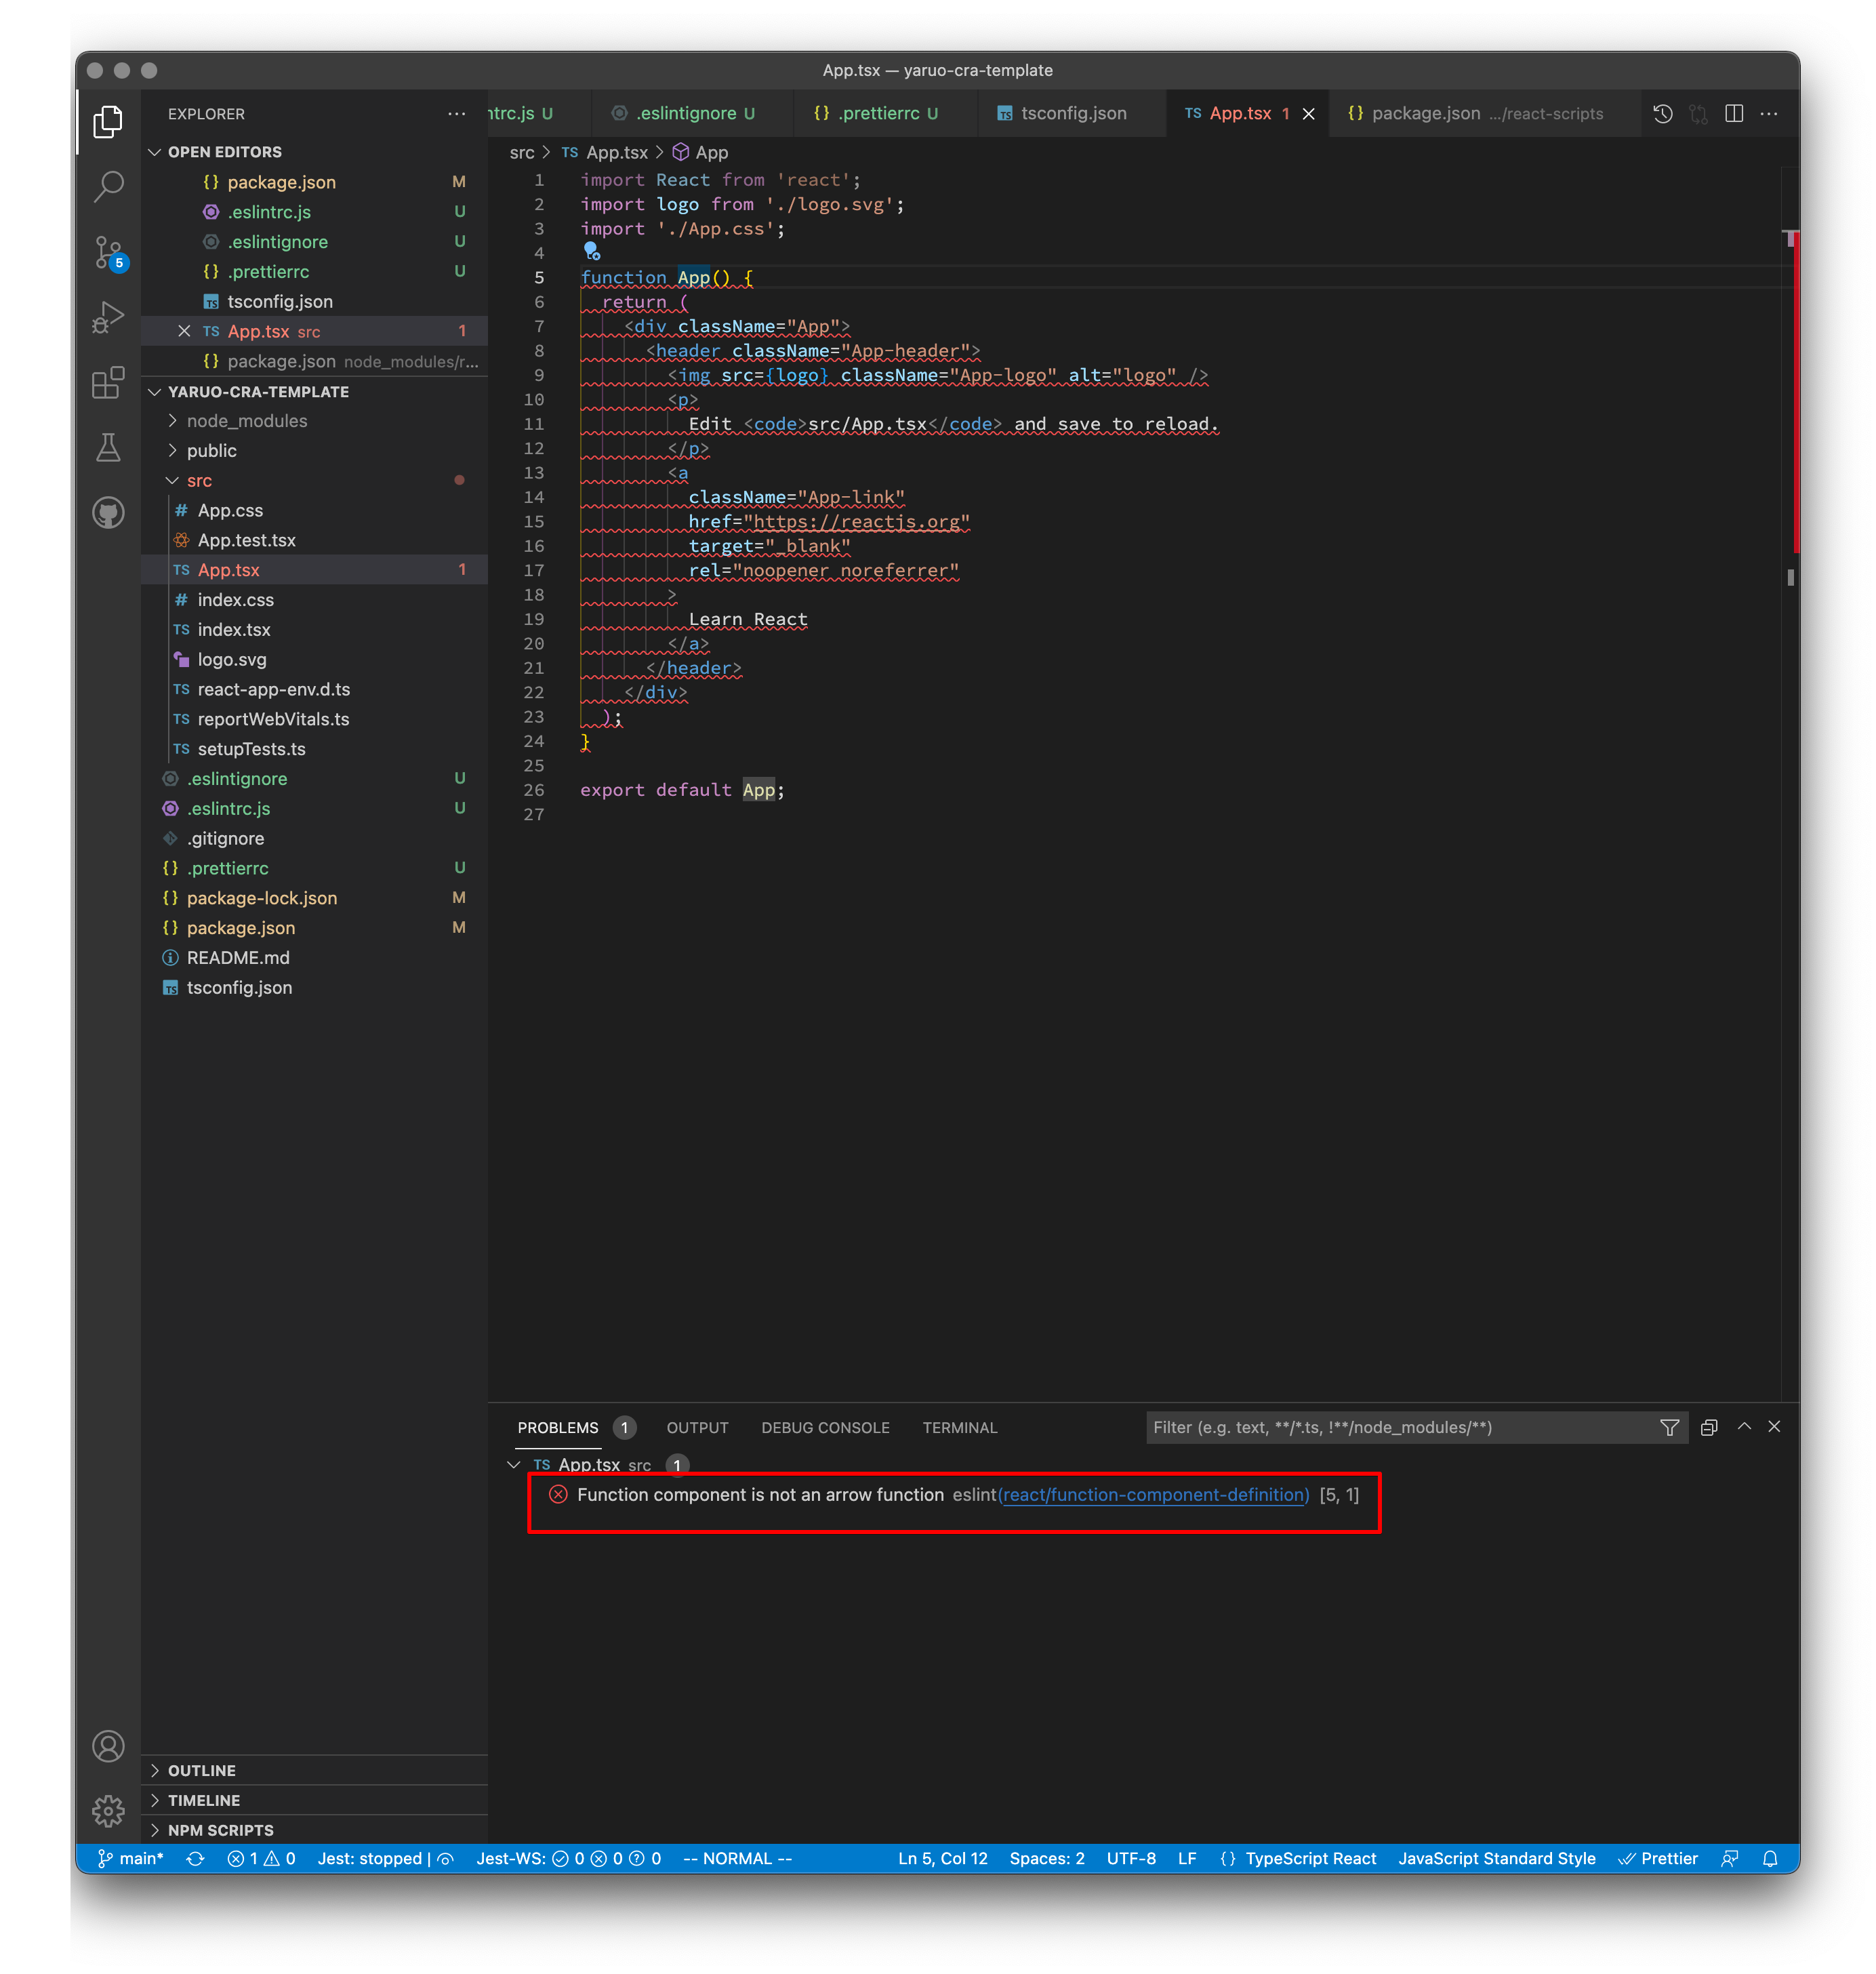
\includegraphics[width=0.8\maxwidth]{./images/02-create-react-app/cra-fix_app_tsx.png}%
\reviewimagecaption{App.tsxの修正}
\label{image:02-create-react-app:cra-fix_app_tsx}
\end{reviewimage}
\begin{starternote}[]{}

筆者がVSCodeを日本語化していないのは、エラーメッセージでググる場合を考えてのことです。
英語でのエラーメッセージの方が的確なページをみつけやすいと考えています。

\end{starternote}

では、指摘されている点を修正していきます。

\def\startercodeblockfontsize{}
\begin{starterprogram}[]{修正後のApp.tsx}\seqsplit{  import React from 'react';
  import logo from './logo.svg';
  import './App.css';

  const App = () =\textgreater{} (
    \textless{}div className='App'\textgreater{}
      \textless{}header className='App{-}header'\textgreater{}
        \textless{}img src=\{logo\} className='App{-}logo' alt='logo' /\textgreater{}
        \textless{}p\textgreater{}
          Edit \textless{}code\textgreater{}src/App.tsx\textless{}/code\textgreater{} and save to reload.
        \textless{}/p\textgreater{}
        \textless{}a
          className='App{-}link'
          href='https://reactjs.org'
          target='\textunderscore{}blank'
          rel='noopener noreferrer'
        \textgreater{}
          Learn React
        \textless{}/a\textgreater{}
      \textless{}/header\textgreater{}
    \textless{}/div\textgreater{}
  );

  export default App;}\end{starterprogram}

次に、「repotWebVitals.ts」でエラーが発生しています。これはimpor文に「void」を付けることで解決します。

\def\startercodeblockfontsize{}
\begin{starterprogram}[]{修正後のreportWebVitals.ts}\seqsplit{  import \{ ReportHandler \} from 'web{-}vitals';

  const reportWebVitals = (onPerfEntry?: ReportHandler) =\textgreater{} \{
    if (onPerfEntry \&\& onPerfEntry instanceof Function) \{
      void import('web{-}vitals').then(
        (\{ getCLS, getFID, getFCP, getLCP, getTTFB \}) =\textgreater{} \{
          getCLS(onPerfEntry);
          getFID(onPerfEntry);
          getFCP(onPerfEntry);
          getLCP(onPerfEntry);
          getTTFB(onPerfEntry);
        \}
      );
    \}
  \};

  export default reportWebVitals;
}\end{starterprogram}

これで現時点での指摘はすべて修正できました。動作確認を行います。

\def\startercodeblockfontsize{}
\begin{starterterminal}[]{create{-}react{-}appの動作確認}\seqsplit{ \textgreater{} npm run start}\end{starterterminal}

これで、トップページが表示されます。

\begin{starternote}[]{}

ここまでの内容は、GitHub上で、以下のコマンドでクローンできます。

\def\startercodeblockfontsize{}
\begin{starterterminal}[]{GitHub}\seqsplit{  \textdollar{} \textgreater{} git clone https://github.com/yaruo{-}react{-}redux/yaruo{-}cra{-}template.git}\end{starterterminal}
\end{starternote}

\section{第2章のまとめ}
\keeplastskip{
  \label{sec:2-5}
  \label{sec-chap02review}
  \par\nobreak
}

Reactを使用しスタートアップ用のアプリケーションの作成方法を

\begin{starteritemize}
\item 「create{-}react{-}app」コマンドで作成
\item ゼロから構築
\end{starteritemize}

の2通りで解説しました。

\vspace*{\baselineskip}

バグの混入を防いだりより良いコーディングをするためにも、ESlint、Prettierを導入しましょう。
